\documentclass[a4paper,10pt]{report}
\usepackage[utf8]{inputenc}
\usepackage{graphicx}
\usepackage{tabularx}
\usepackage[table]{xcolor}
\usepackage{background}
\usepackage{fontspec}
\usepackage{hyperref}
\usepackage{multicol}
\usepackage{caption}
\usepackage{subcaption}
\usepackage{a4wide}
\usepackage{makecell}
\usepackage{pdfpages}
\setmainfont{Sweet Sans Pro}
\definecolor{cream1}{RGB}{242,241,234}
\definecolor{cream2}{RGB}{232,231,224}
\hypersetup{
    colorlinks=true,
    linkcolor=black,
    filecolor=magenta,
    urlcolor=cyan,
    pdftitle={HW-T4-50F user manual},
    pdfpagemode=FullScreen,
    }
\backgroundsetup{
scale=1,
color=black,
opacity=0.9,
angle=0,
contents={%
  
\includegraphics[width=\paperwidth,height=\paperheight]{images/page.png}
  }%
}
%opening
\title{HW-T4-50F user manual}
\author{Abdellah Radad}

\begin{document}
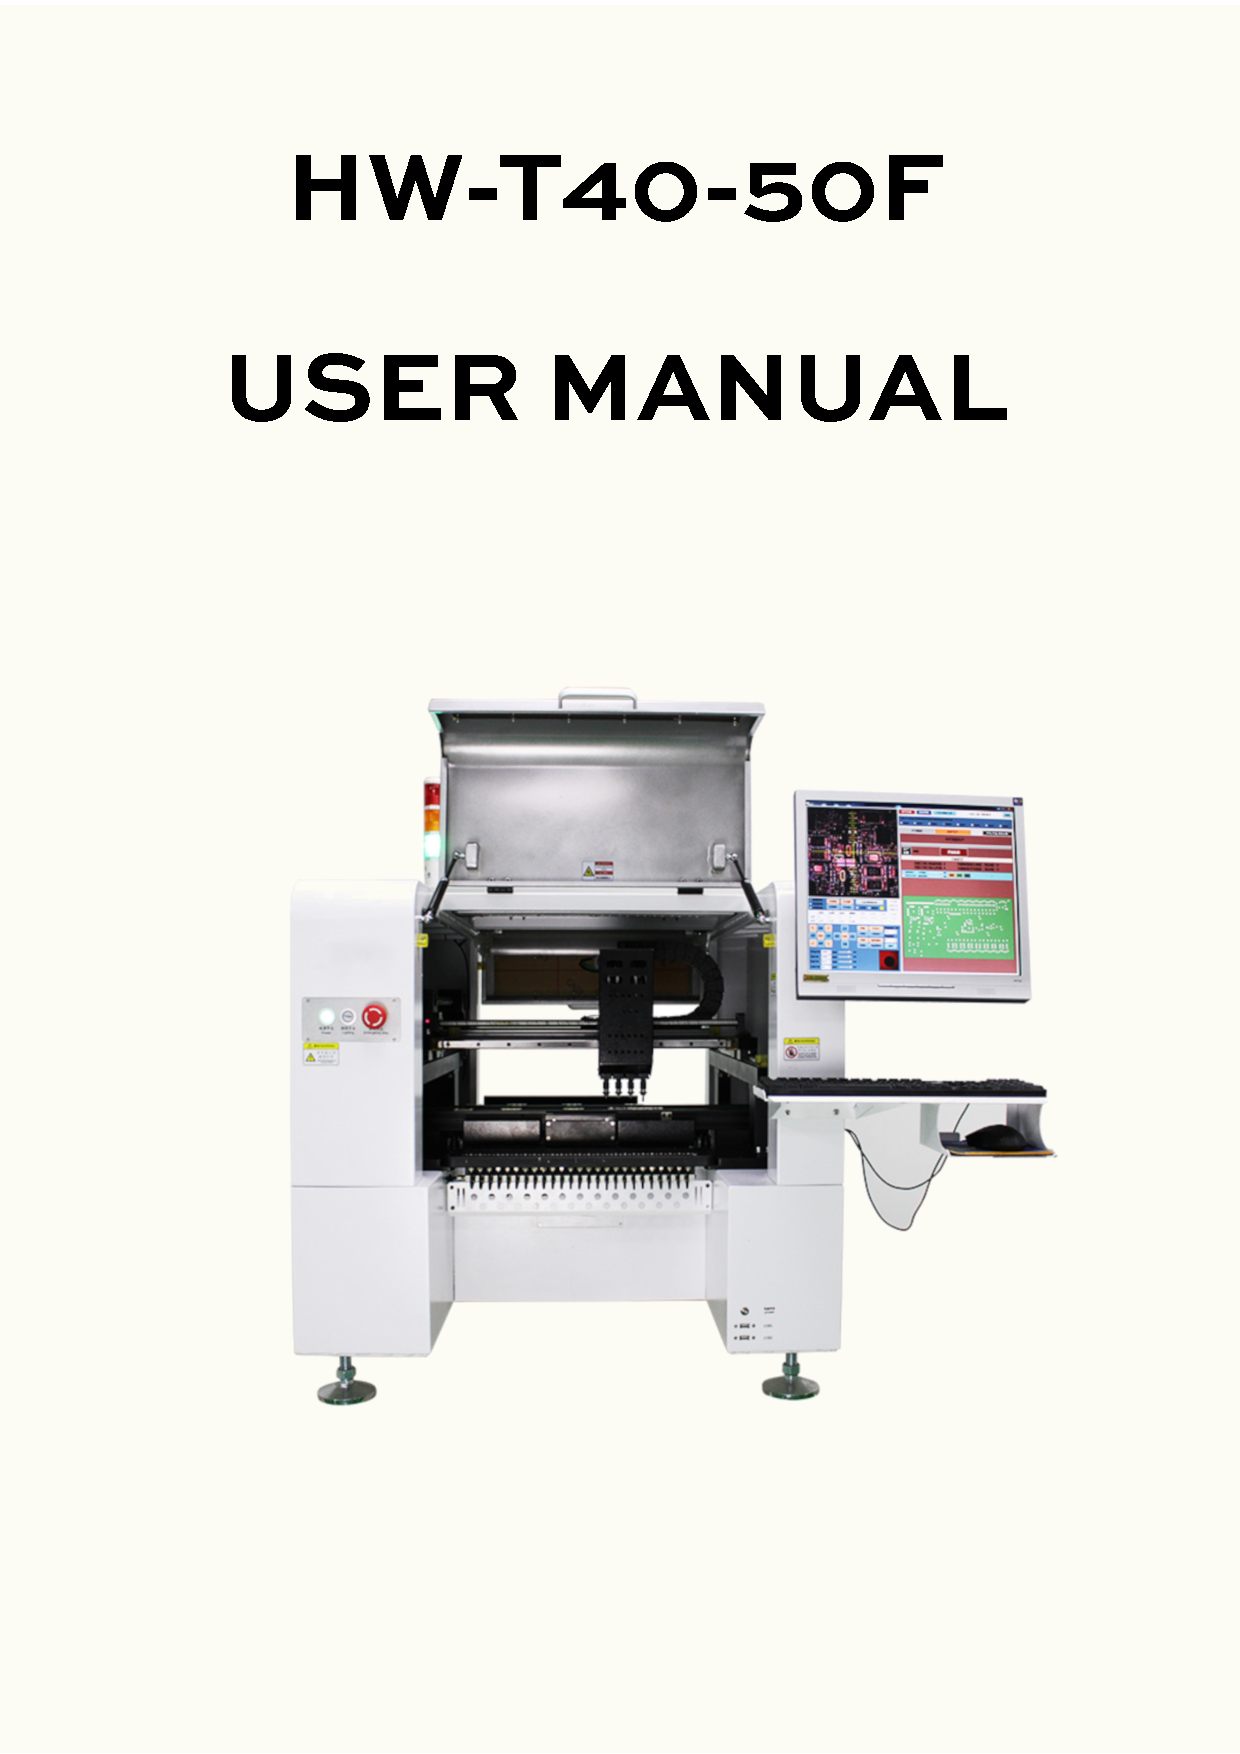
\includepdf{frontpage.pdf}
\newpage
\tableofcontents
\newpage
\listoffigures
\newpage
\chapter{HW-T4-50F user manual}
\newpage
\section{Introduction to the HW-T4-50F}
The Huawei T4-50F is an 50 feeder / 4 nozzle pick and place machine. It can be operated manually or via pick and place csv files generated by the user's EDA suite of choice.\\
\subsection{Hardware overview}
\subsubsection{- The pick and place arm}
\begin{figure}[!htb]
 \centering
 \includegraphics[width=0.85\textwidth]{images/arm.png}
 \caption{HW-T4-50F pick and place arm}
\end{figure}
The HW-T4-50F's main component is the pick and place arm. It allows movement across the XY plane, and contains 4 placement heads equipped with 4 nozzles.\\
It is also home to the \textbf{Mark Cam}, \textbf{Mark Light} and \textbf{Mark LED}.
\newpage
\subsubsection{- The cameras}
The mark cam is a camera installed on the pick and place arm of the HW-T4-50F, it is most often used for calibration and fiducial mark recognition purposes.\\
\begin{figure}[!htb]
 \centering
 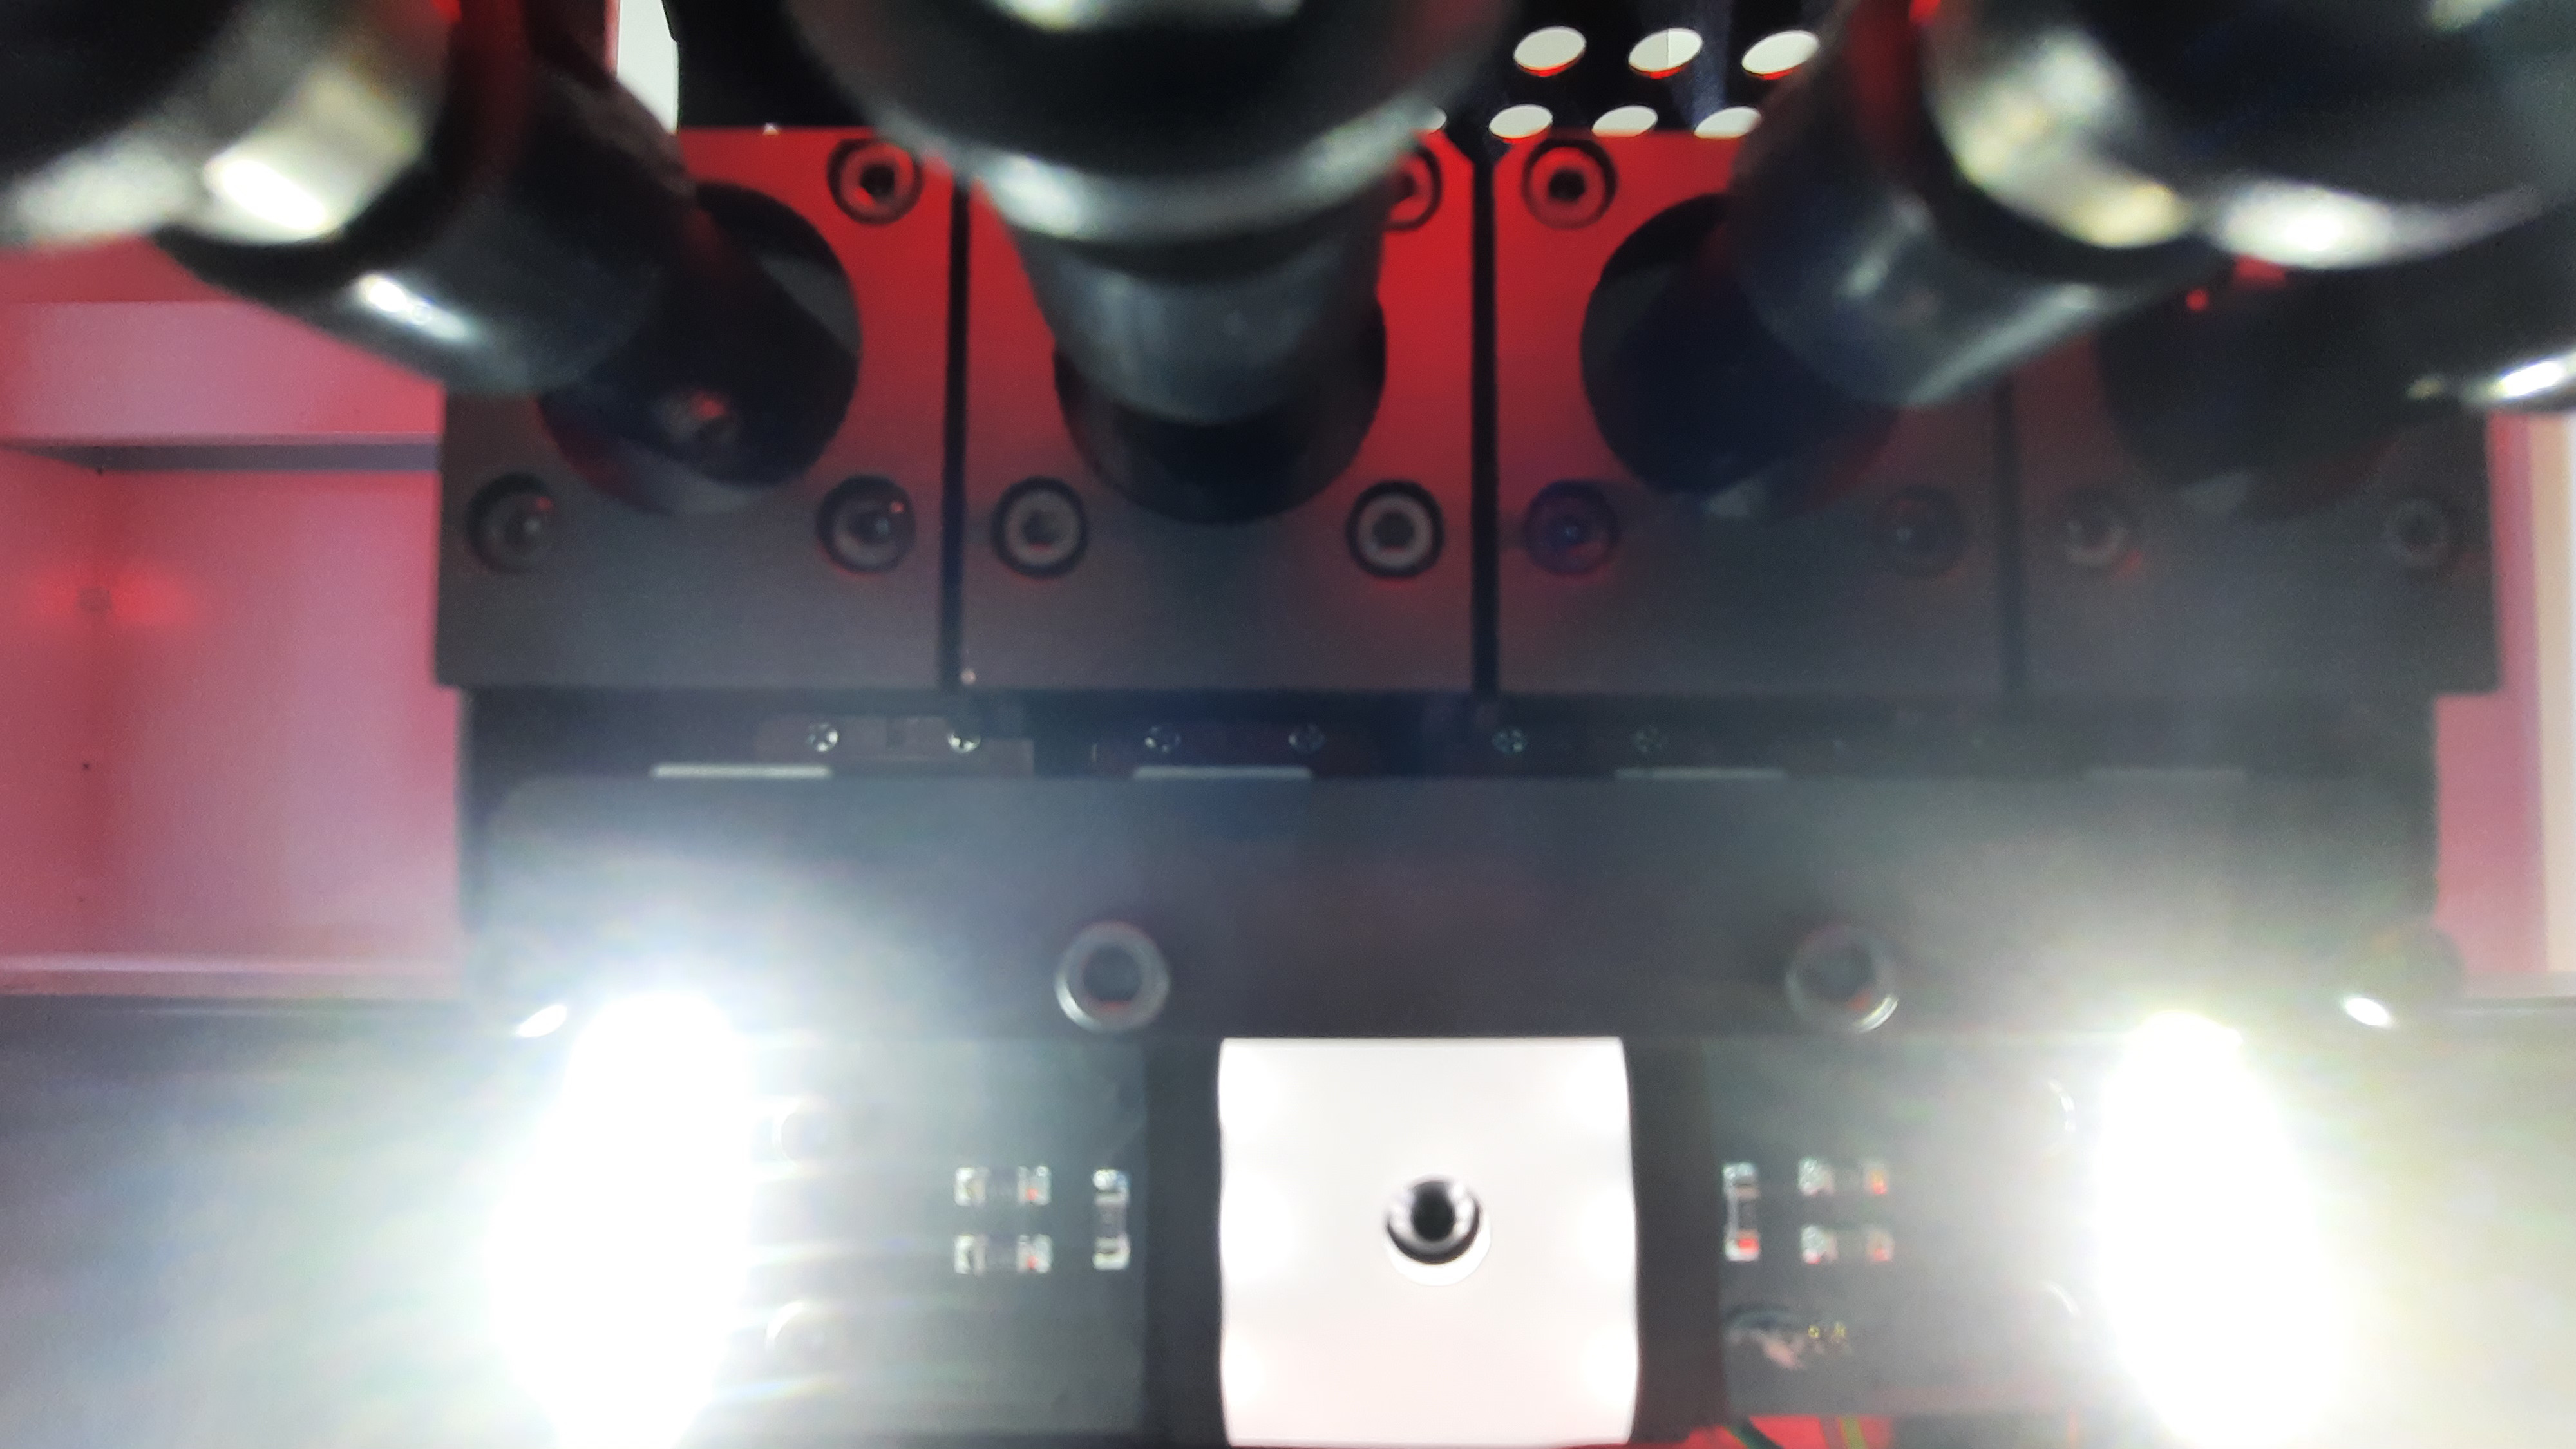
\includegraphics[width=0.75\textwidth]{images/mcam.jpg}
 \caption{Mark Cam}
\end{figure}

The fast cam is mounted on the HW-T4-50F chassis. It is comprised of four cameras, one for each nozzle.\\
The fast cam's main role is component visual inspection.
\begin{figure}[!htb]
 \centering
 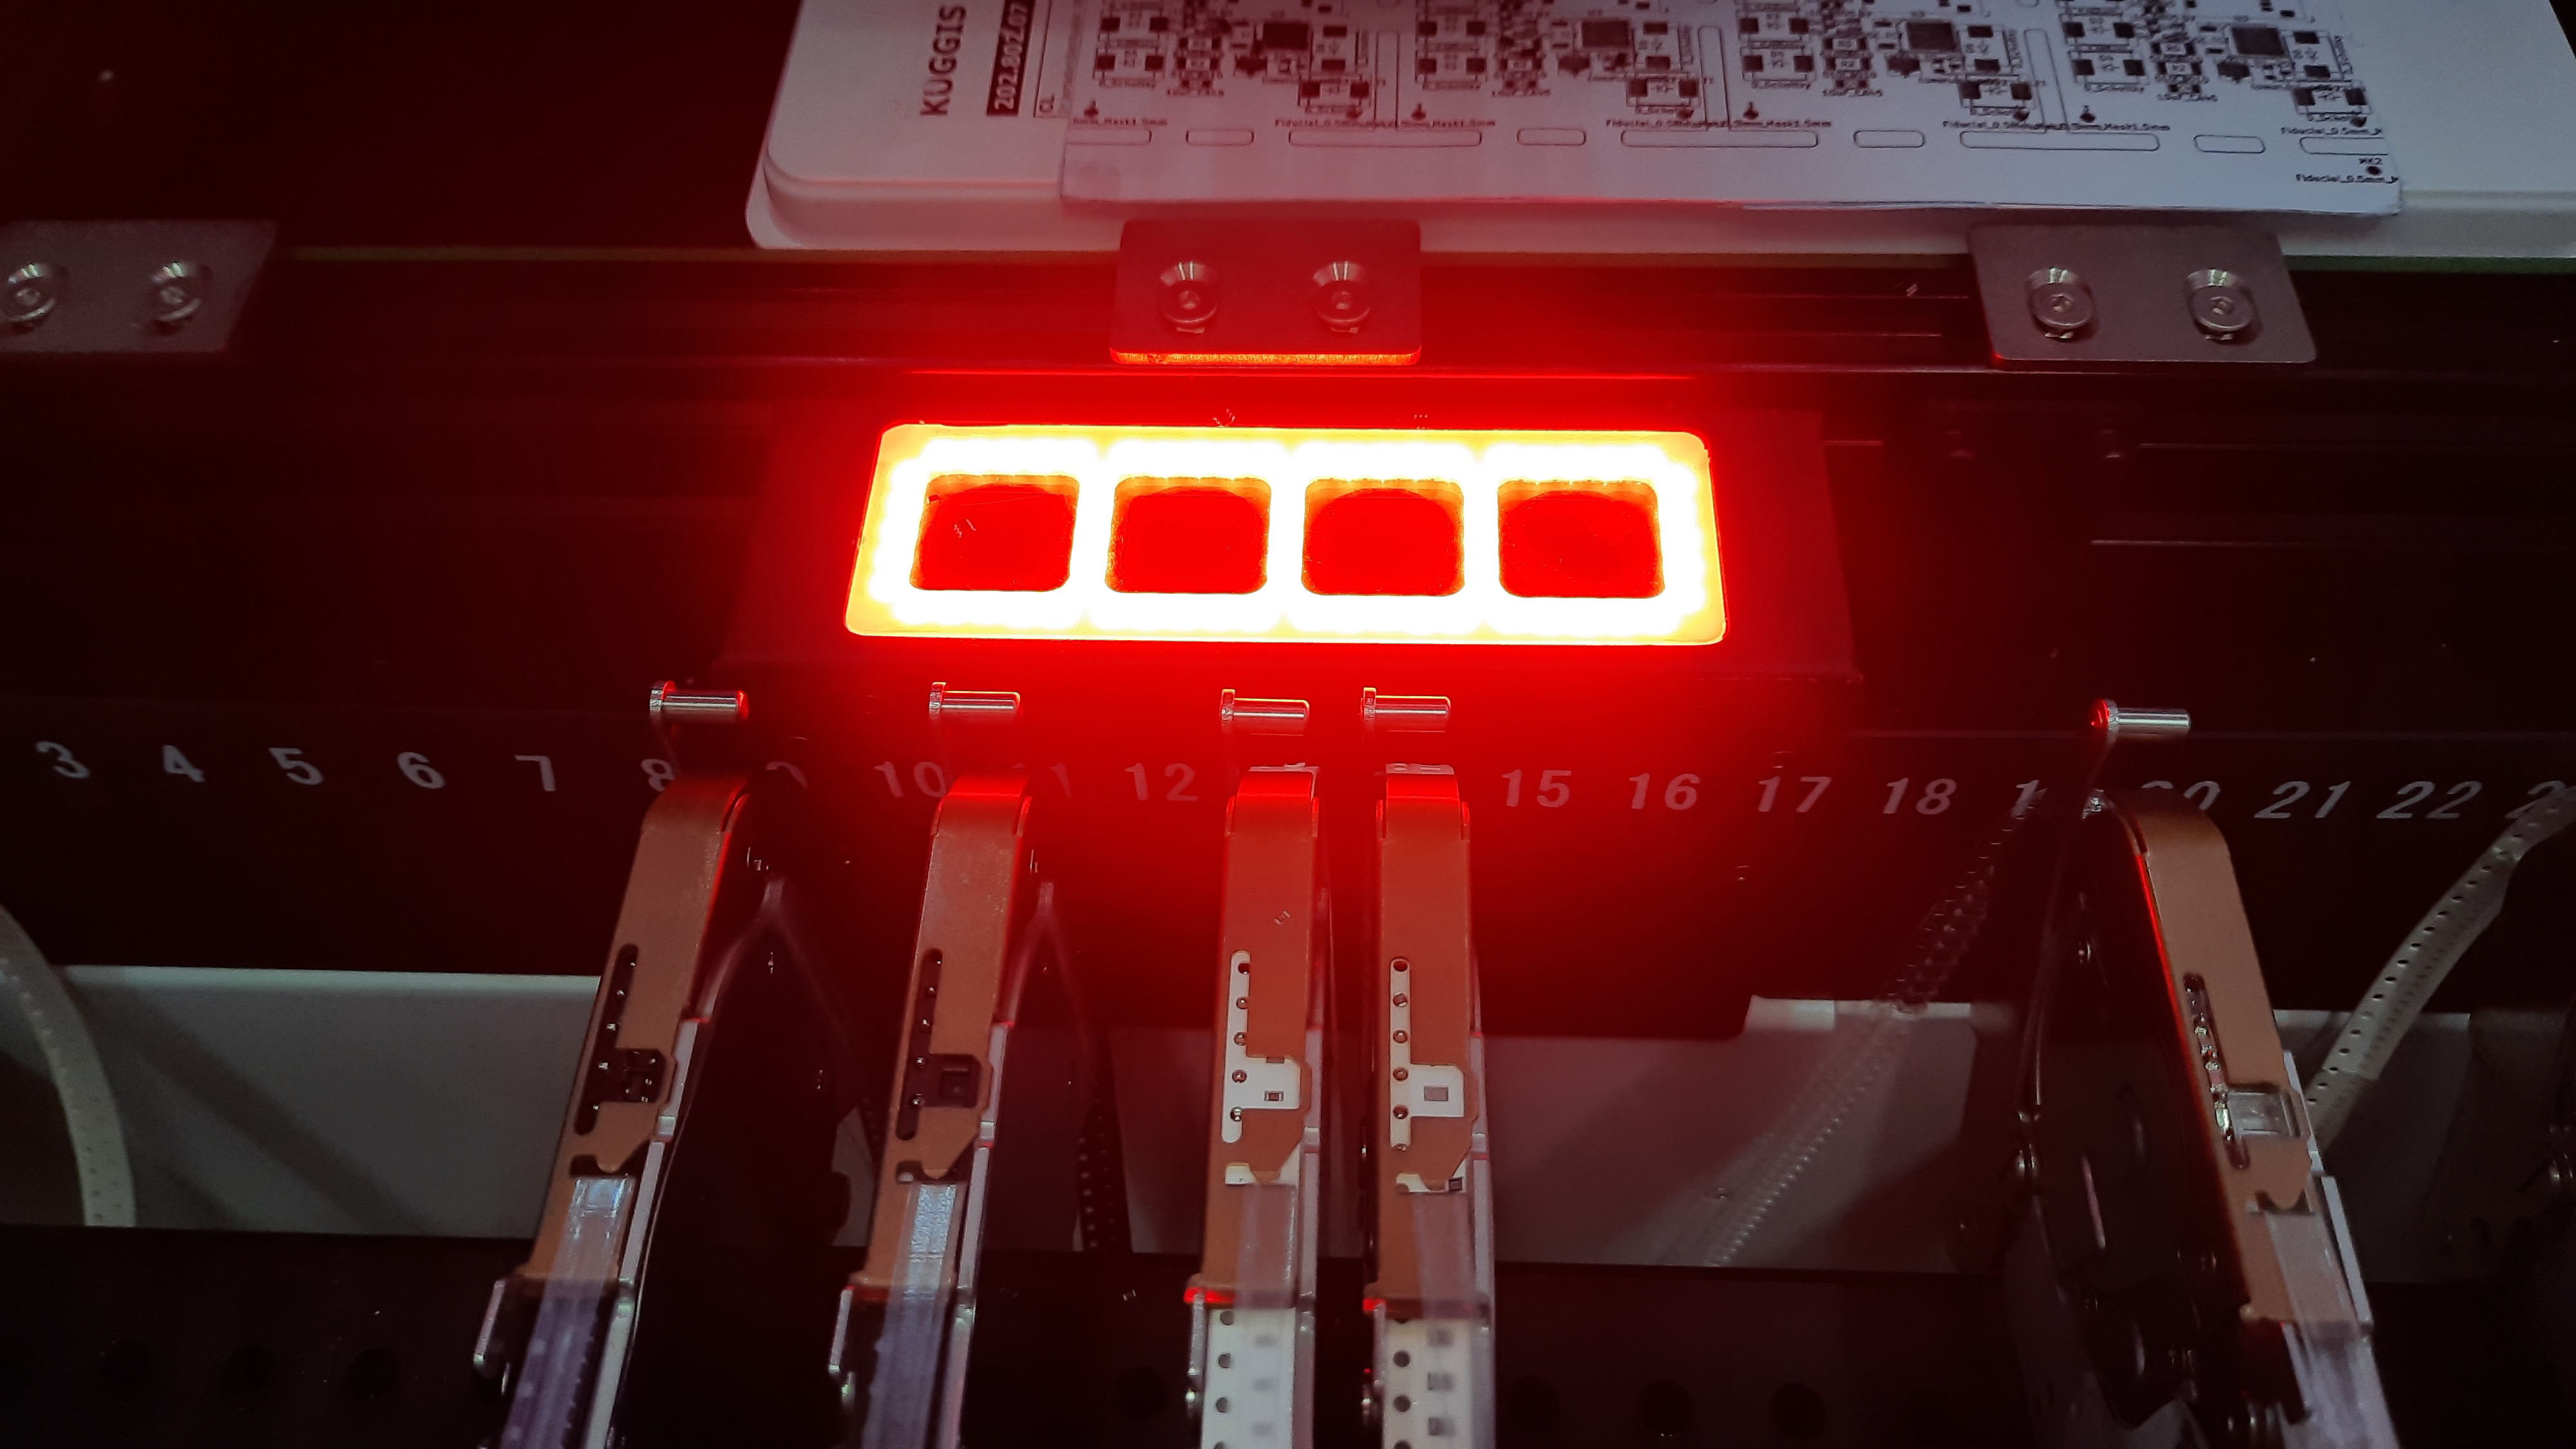
\includegraphics[width=0.75\textwidth]{images/fcam.jpg}
 \caption{Fast Cam}
\end{figure}

\newpage
The high cam is mounted on the HW-T4-50F chassis. It's a single camera used for component visual inspection.\\
\begin{figure}[!htb]
 \centering
 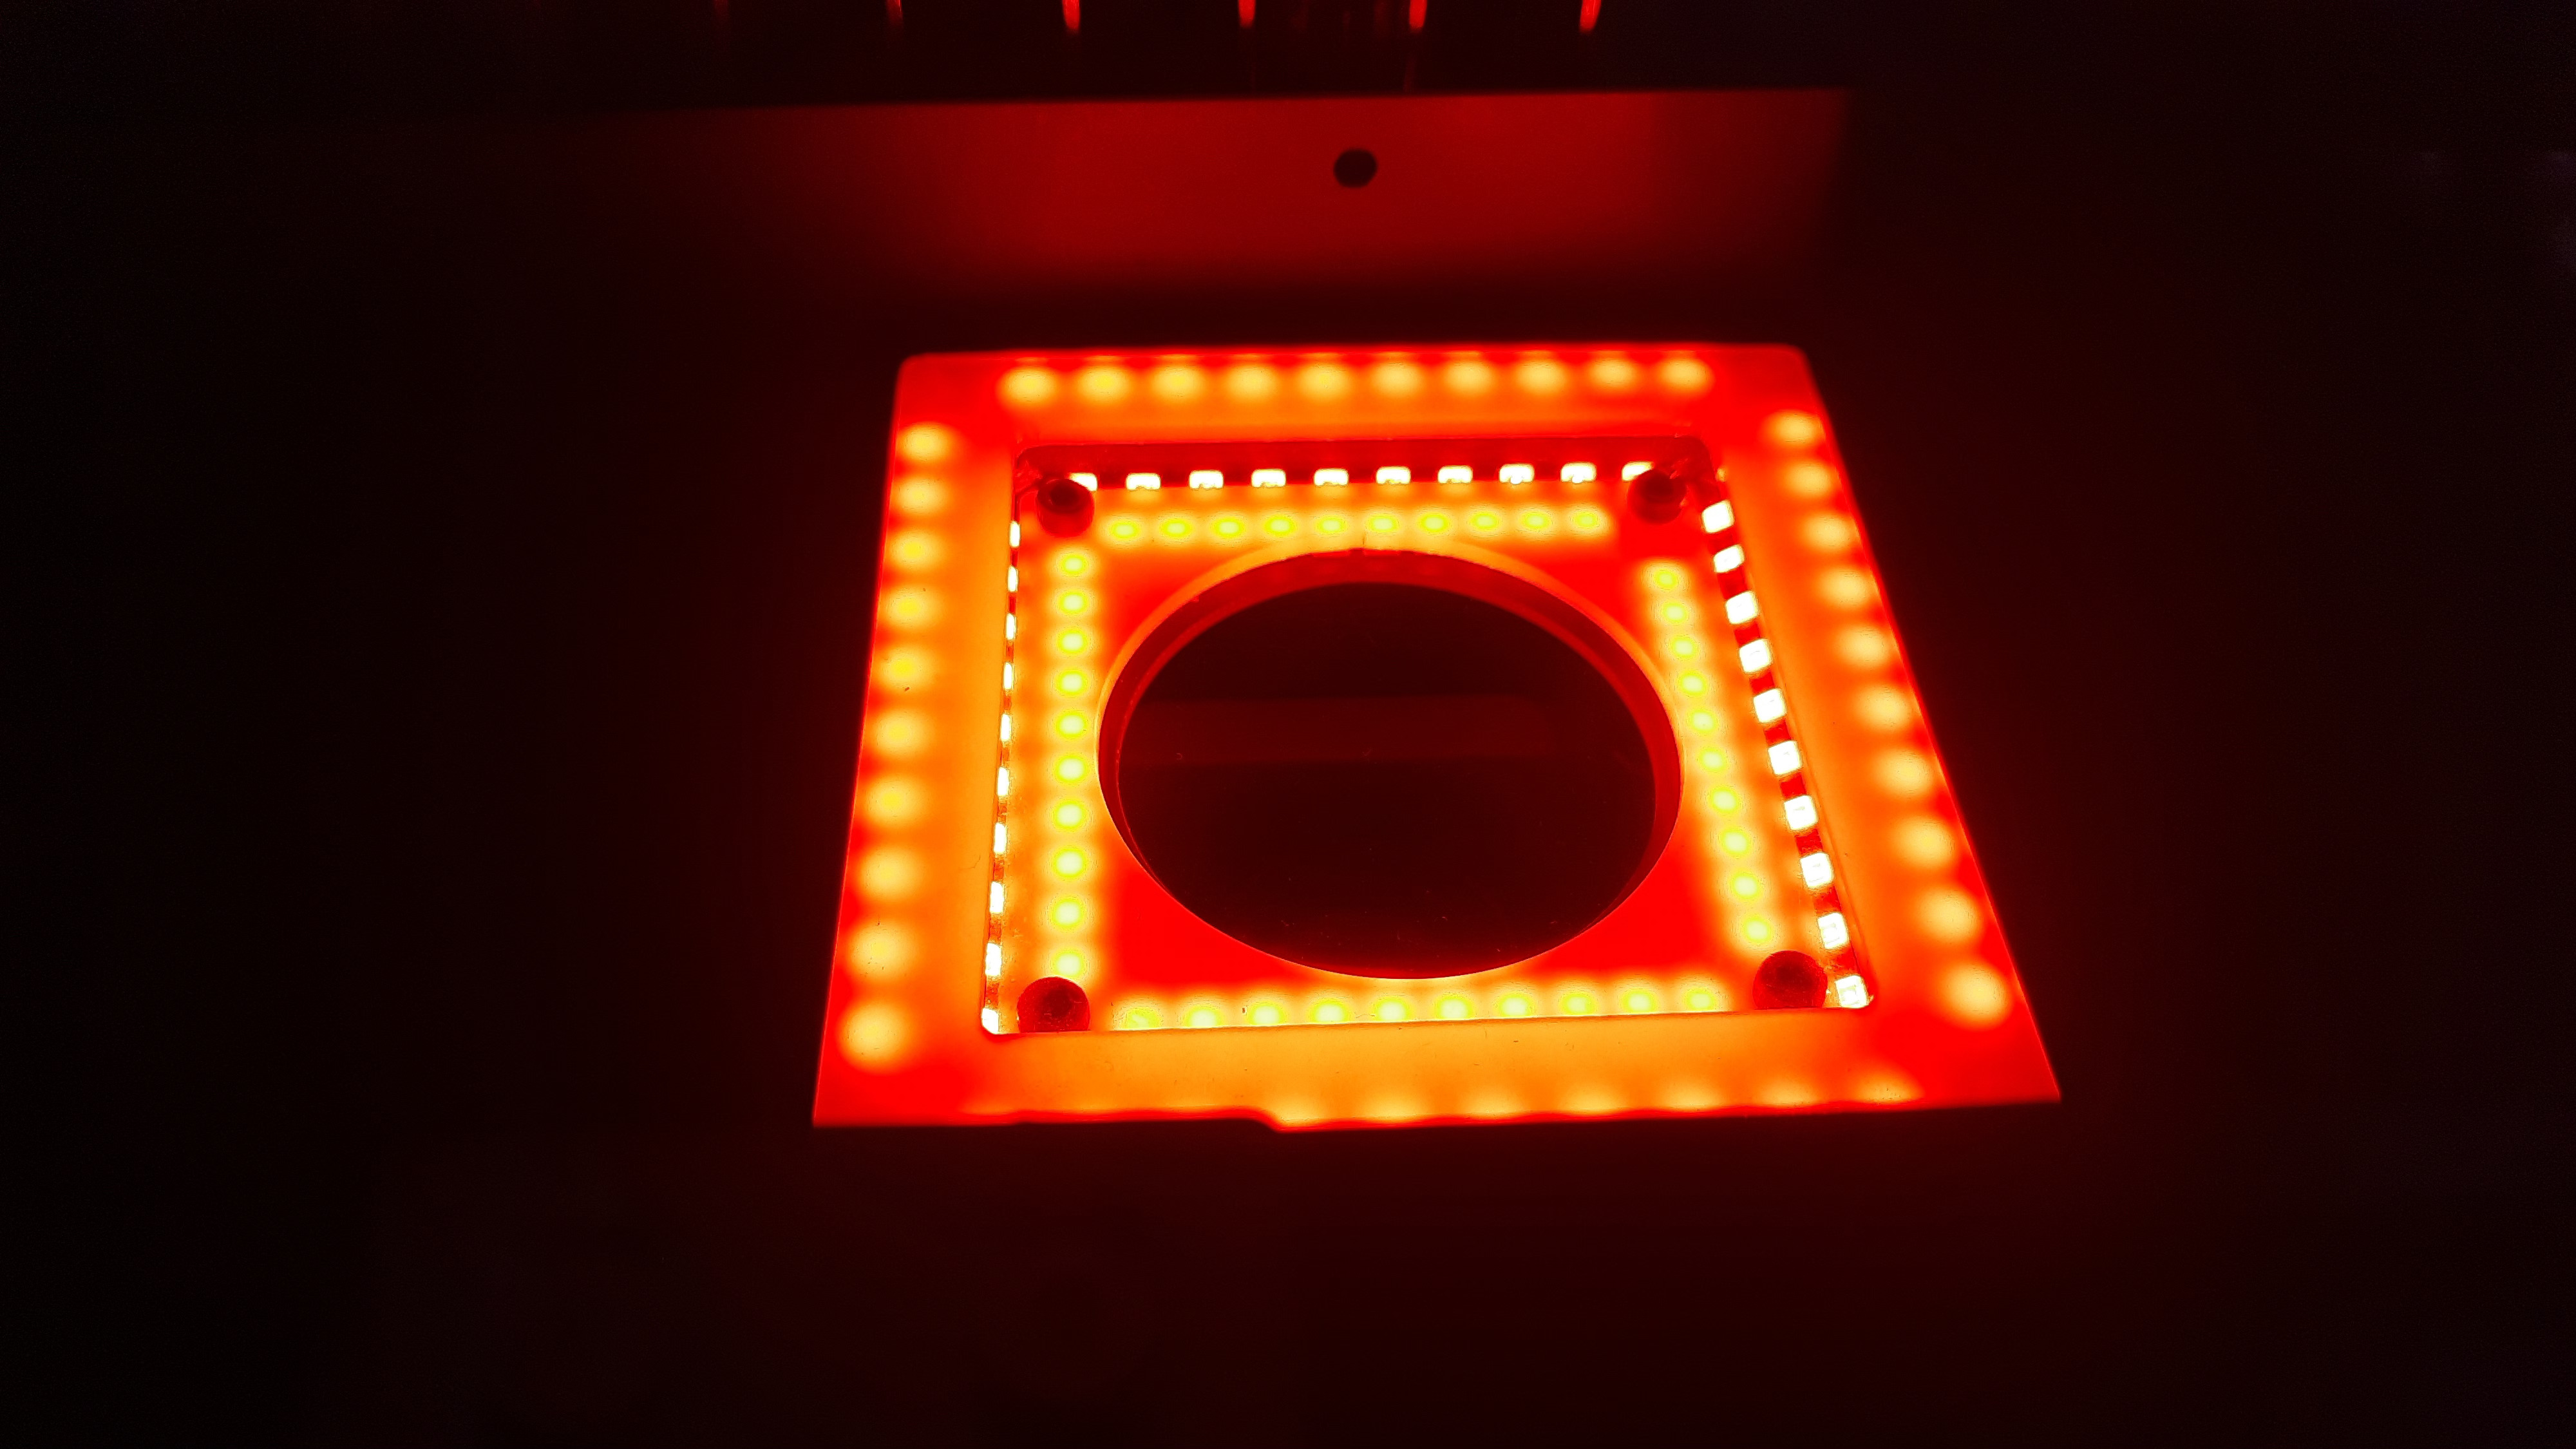
\includegraphics[width=0.85\textwidth]{images/hcam.jpg}
 \caption{High Cam}
\end{figure}


\newpage
\section{Terminology}
\begin{itemize}
 \item \textbf{PCB Array: } A PCB array (also called a PCB panel) is a PCB  grid containing multiple smaller boards \textbf{identical} in design.
 \item \textbf{Coupled PCB Array: } A PCB array in a 2xN or Nx2 shape, which may or may not be mirrored.
 \item \textbf{Arm: } In the document, the arm is the part of the pick and place machine that contains the \textbf{Mark Cam}, placement heads and nozzles.
 \item \textbf{Reel: } The reel is a circular spool around which the carrier tape is wound.
 \item \textbf{Carrier tape: }  The carrier tape is a continuous strip that holds the electronic components. It consists of a series of pockets or cavities where individual components are placed. The tape also includes sprocket holes along its edges for precise alignment and advancement through the pick and place machine.
 \item \textbf{Cover tape: } A translucent film that holds the components inside the Carrier tapes' pockets.
 \item \textbf{Pick up height: } The height to which the nozzle must come down to pick up a component.
  \item \textbf{Place height: } The height to which the nozzle must descend to place a component on the pcb.
\end{itemize}
\newpage

\section{Relevant product specifications}
\subsection{Relevant product specifications table}
\begin{table}[!htb]
{\rowcolors{1}{cream1}{cream2}
\begin{tabularx}{\textwidth}{>{\bfseries}l|X}
 \hline
 Placement head count & 4 \\
 \hline
 Number of feeder slots & 50 \\
 \hline
 Positioning Accuracy & 0.01mm \\
 \hline
 Repeated Mounting Accuracy & 0.02mm \\
 \hline
 Range of Mounting Speed & 7000-8000Pcs/h\\
 \hline
 Supported Maximum Area of PCB & 350*190mm \\
 \hline
 Applicable components & 0201, 0402, 0603, 0805, diode , triode, SOT and QFP ,
BGA with lead pitch $\geq 3mm$  \\
 \hline
 Maximum Height of Components & $\leq 7mm $\\
 \hline
 Mark Positioning & manual / automatic\\
 \hline
 Maximum Step Length of XY Axis & 629mm*679mm\\
 \hline
 Maximum Step Length of Z Axis & 20mm\\
 \hline
 Power Supply & 220V 50/60Hz\\
 \hline
 Average Power & 600W\\
 \hline
\end{tabularx}}
\end{table}


\subsection{Specification details}

\subsubsection{Placement heads}
In the context of P\&P machines, placement heads use nozzles to pick up and hold components.\\
Nozzles use a vacuum system to pick components of the feeder and place them on the pcb.
The HW-T4-50F possesses 4 placement heads.
\begin{figure}[!htb]
 \centering
 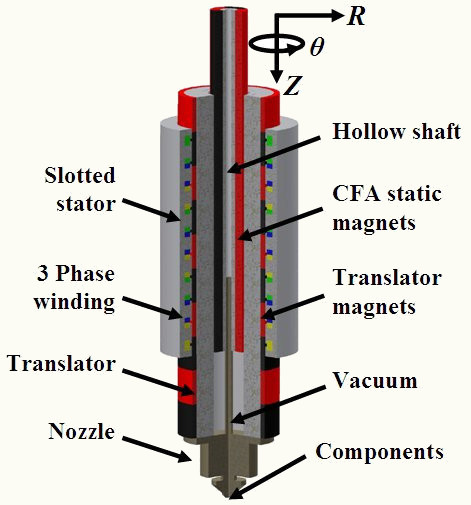
\includegraphics[width=0.45\textwidth]{images/placement_head.jpg}
 \caption{A P\&P placement head}
\end{figure}
\newpage
\begin{table}[!htb]
\centering
{\rowcolors{1}{cream1}{cream2}
\resizebox{\textwidth}{!}{\begin{tabularx}{\textwidth}{|>{\bfseries}l|c|c|c|c|}
\hline
Component Type & Designation & Length (μm) & Width (μm) & Nozzle Type \\
\hline
\multicolumn{5}{|l|}{\textbf{Flat Chip}} \\
\hline
 & 0201 & 600 & 300 & 501 \\
 & 0402 & 1000 & 500 & 502 \\
 & 0603 & 1600 & 800 & 503 \\
 & 0805 & 2000 & 1250 & 503 \\
 & 1206 & 3200 & 1600 & 504 \\
 & 1210 & 3200 & 2600 & 505 \\
 & 2010 & 5000 & 2500 & 505 \\
 & 2512 & 6300 & 3100 & 505 \\
\hline
\multicolumn{5}{|l|}{\textbf{MELFs}} \\
\hline
 & 2000 & \phi 1350 & - & 510 \\
 & 3200 & \phi 1750 & - & 510 \\
 & 3500 & \phi 1550 & - & 510 \\
 & 5900 &\phi 2400 & - & 511 \\
\hline
\multicolumn{5}{|l|}{\textbf{Tantalum Capacitors, Inductors, Potentiometers}} \\
\hline
Potentiometer & 3000 & 3400 & 1500 & 505 \\
 & 3800 & 4500 & 1650 & 506 \\
 & 4000 & 4500 & 2400 & 506 \\
Inductor Chip & 2500 & 2000 & 1800 & 504 \\
 & 3200 & 2500 & 2200 & 505 \\
 & 4000 & 4300 & 4300 & 506 \\
Tantalum Capacitor & 2000 & 1250 & 1200 & 503 \\
 & 3200 & 1600 & 1600 & 504 \\
 & 3400 & 2600 & 1900 & 505 \\
\hline
\multicolumn{5}{|l|}{\textbf{Electrolytic Capacitors}} \\
\hline
 & 3300 & \phi 3000 & 5400 & 505 \\
 & 4300 & \phi 4000 & 5400 & 506 \\
 & 5300 & \phi 5000 & 5400 & 506 \\
 & 6600 & \phi 6300 & 5400 & 506 \\
 & 6600 & \phi 6300 & 7900 & 506 \\
 & 8300 & \phi 8000 & 6200 & 507 \\
 & 8300 & \phi 8000 & 10200 & 507 \\
 & 10300 & \phi 10000 & 10200 & 508 \\
\hline
\multicolumn{5}{|l|}{\textbf{Transistors, Diodes}} \\
\hline
Transistor SC90 & 1600 & 800 & 700 & 503 \\
Transistor SOT323 & 2000 & 1250 & 900 & 503 \\
 & 2000 & 1250 & 1100 & 503 \\
 & 2900 & 1300 & 950 & 503 \\
 & 2900 & 1600 & 950 & 504 \\
 & 2900 & 1600 & 1100 & 504 \\
Transistor DPAK & 9900 & 6500 & 4700 & 506 \\
Diode SOD123 & 3700 & 1550 & 1400 & 504 \\
Diode SOD323 & 2500 & 1250 & 1200 & 503 \\
\hline
\end{tabularx}}}
\caption{SMT Nozzle Selection Guide}
\end{table}
\newpage
\begin{table}[!htb]
\centering

{\rowcolors{1}{cream1}{cream2}
\resizebox{\textwidth}{!}{\begin{tabularx}{\textwidth}{|>{\bfseries}l|X|X|X|X|}
\multicolumn{5}{|l|}{\textbf{Small Outlines}} \\
\hline
SO6 * 1.27p & 3800 & 6000 & 1450 & 506 \\
SO8 * 1.27p & 4900 & 6000 & 1550 & 506 \\
SO14 * 1.27p & 8650 & 6000 & 1550 & 506 \\
SO16 * 1.27p & 10000 & 6000 & 1600 & 506 \\
SO8L * 1.27p & 8000 & 10300 & 2500 & 508 \\
SO14L * 1.27p & 9100 & 10320 & 2500 & 508 \\
SO16L * 1.27p & 10280 & 10300 & 2500 & 508 \\
SO18L * 1.27p & 11550 & 10300 & 2500 & 508 \\
SO20L * 1.27p & 12800 & 10325 & 2500 & 508 \\
SO24L * 1.27p & 15400 & 10325 & 2500 & 508 \\
SO28L * 1.27p & 18000 & 10300 & 2450 & 508 \\
SO32L * 1.27p & 21000 & 10600 & 2670 & 508 \\
SO40L * 1.27p & 26600 & 11800 & 2900 & 508 \\
SOJ24 * 1.27p & 15880 & 8660 & 3500 & 507 \\
SOJ26 * 1.27p & 17150 & 8660 & 3500 & 507 \\
SOJ28 * 1.27p & 18410 & 8660 & 3500 & 507 \\
SOJ32 * 1.27p & 20960 & 8510 & 3500 & 507 \\
TSOP24 * 0.5p & 16000 & 6000 & 1200 & 506 \\
TSOP32 * 0.5p & 20000 & 8000 & 1000 & 507 \\
TSOP40 * 0.5p & 20000 & 10100 & 1200 & 508 \\
SSOP8 * 0.65p & 3000 & 7800 & 1800 & 507 \\
SSOP14* 0.65p & 6200 & 7800 & 1800 & 507 \\
SSOP16 * 0.65p & 6200 & 7800 & 1800 & 507 \\
SSOP18 * 0.65p & 7200 & 7800 & 1800 & 507 \\
SSOP20 * 0.65p & 7200 & 7800 & 1800 & 507 \\
SSOP22 * 0.65p & 9200 & 7800 & 1800 & 507 \\
SSOP24 * 0.65p & 9200 & 7800 & 1800 & 507 \\
SSOP28 * 0.65p & 10200 & 7800 & 1800 & 507 \\
SSOP30 * 0.65p & 10200 & 7800 & 1800 & 507 \\
SSOP34 * 0.65p & 118100 & 10250 & 2600 & 508 \\
SSOP36 * 0.65p & 15600 & 10350 & 2600 & 508 \\
SSOP38 * 0.65p & 12600 & 7800 & 1800 & 507 \\
SSOP44 * 0.65p & 17900 & 10300 & 2515 & 508 \\
SSOP48 * 0.65p & 15880 & 10310 & 2590 & 508 \\
SSOP56* 0.65p & 18400 & 19350 & 2600 & 508 \\
SSOP64 * 0.65p & 26300 & 14250 & 2100 & 508 \\
\hline
\multicolumn{5}{|l|}{\textbf{Plastic Leaded Chip Carriers}} \\
\hline
PLCC20 *1.27p & 9850 & 9850 & 4350 & 507 \\
\end{tabularx}}}
\caption{SMT Nozzle Selection Guide}
\end{table}
\newpage
\subsubsection{- Feeders}
A feeder is the system responsible for supplying the P\&P placement head with components. Feeders are usually divided into 4 main categories:
\begin{itemize}
    \item \textbf{Tape Feeders}
    \begin{itemize}
        \item \textbf{Description:} Use reels of carrier tape holding components in pockets.
        \item \textbf{Types:}
        \begin{itemize}
            \item \textbf{Embossed Tape Feeders:} For larger or irregularly shaped components.
            \item \textbf{Paper Tape Feeders:} For small, lightweight components.
        \end{itemize}
        \item \textbf{Advantages:} High component density, suitable for high-speed placement.
        \item \textbf{Use Case:} Widely used for a variety of surface-mount devices (SMDs).
    \end{itemize}

    \item \textbf{Tube Feeders}
    \begin{itemize}
        \item \textbf{Description:} Components stored in tubes and fed one by one.
        \item \textbf{Types:}
        \begin{itemize}
            \item \textbf{Vibratory Tube Feeders:} Use vibration to move components to the pick position.
            \item \textbf{Mechanical Tube Feeders:} Use mechanical pushers to move components.
        \end{itemize}
        \item \textbf{Advantages:} Simple and reliable for specific component shapes.
        \item \textbf{Use Case:} Used for ICs, transistors, and connectors.
    \end{itemize}

    \item \textbf{Tray Feeders}
    \begin{itemize}
        \item \textbf{Description:} Components stored in trays (JEDEC trays) and presented in an organized manner.
        \item \textbf{Types:}
        \begin{itemize}
            \item \textbf{Manual Tray Feeders:} Trays manually loaded and unloaded.
            \item \textbf{Automatic Tray Feeders:} Trays automatically managed by the machine.
        \end{itemize}
        \item \textbf{Advantages:} Suitable for larger components and sensitive components.
        \item \textbf{Use Case:} Used for large ICs, BGA, and QFP components.
    \end{itemize}


    \item \textbf{Bulk Feeders}
    \begin{itemize}
        \item \textbf{Description:} Components stored in bulk and fed using vibratory/centrifugal mechanisms.
        \item \textbf{Advantages:} Efficient for high volumes of small components.
        \item \textbf{Use Case:} Suitable for small components like capacitors, resistors, and LEDs.
    \end{itemize}
\end{itemize}
Tape/Reel feeders are reserved for smaller components ($\leq 1mm$) while tray feeders are generally reserved for larger chips like microcontrollers and GSM modules.\\
\newpage
The HW-T4-50F has 50 feeder slots. It is important to take into account that vibratory tube feeders occupy \textbf{5 slots}, and tray feeders must be put in a position within the pick and place arms' reach.
\begin{figure}[!htb]
 \centering
 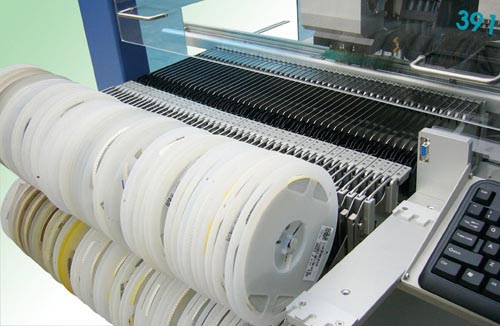
\includegraphics[width=0.85\textwidth]{images/reel_tape.jpg}
 \caption{Reel feeder}
\end{figure}
\subsubsection{- Positioning accuracy}
Positioning accuracy refers to the ability of the pick-and-place machine to place a component at a specified location on the PCB with precision. It is a measure of how close the actual placement of the component is to the intended placement coordinates.\\ \textbf{The HW-T4-50F's positioning accuracy is 0.01mm.}
\subsubsection{- Repeated mounting accuracy}
Repeated mounting accuracy, also known as repeatability, refers to the ability of the pick-and-place machine to consistently place components at the same location on the PCB over multiple cycles. It is a measure of the machine's consistency and reliability in placing components.\\ \textbf{The HW-T4-50F's  repeated mounting accuracy is 0.02mm.}
\newpage
\section{Interfacing with the machine}
\subsection{Front controls}
On the front of the machine are three toggle buttons.
\begin{itemize}
 \item \textbf{Power: } to toggle the machine's power.
 \item \textbf{Lighting: } to turn on the machine's internal lights.
 \item \textbf{Emergency stop: } which stops the machine immediately in the case of an emergency
\end{itemize}
 \begin{figure}[!htb]
 \centering
 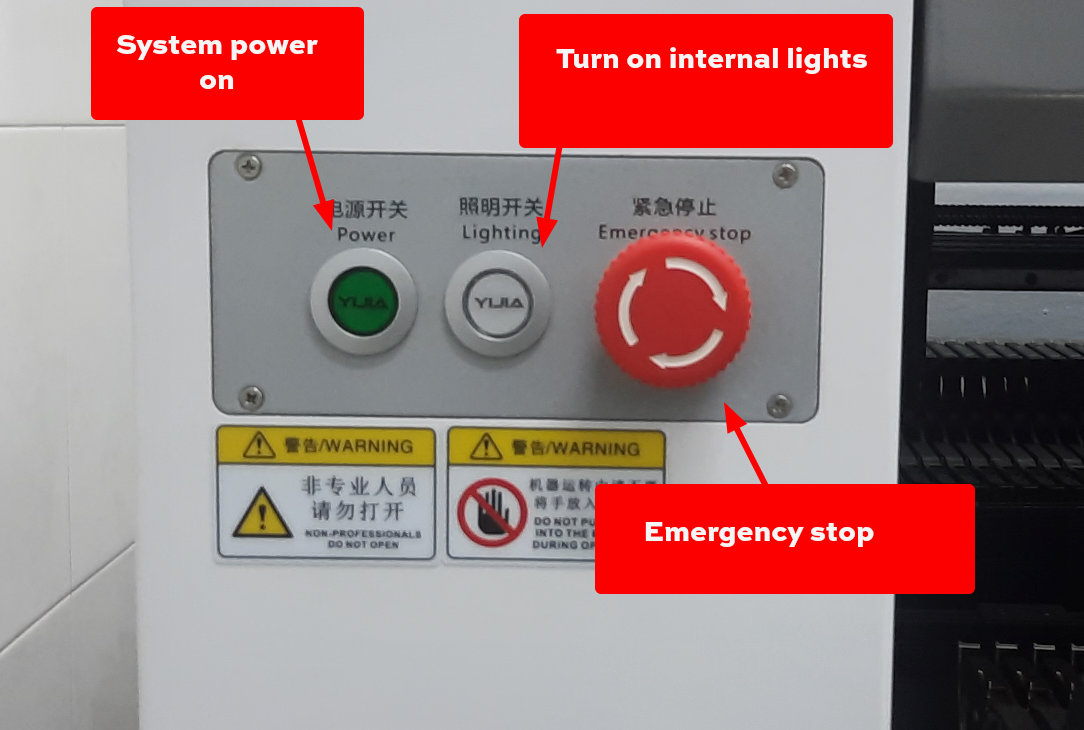
\includegraphics[width=1\textwidth]{images/face_panel.png}
 \caption{HW-T4-50F's face controls}
\end{figure}
\newpage
\subsection{Human Machine Interface}
Powering the HW-T4-50F is a windows 7 computer, containing the needed software, which can be interfaced with via the provided monitor (Keyboard/Mouse arent usually included).
 \begin{figure}[!htb]
 \centering
 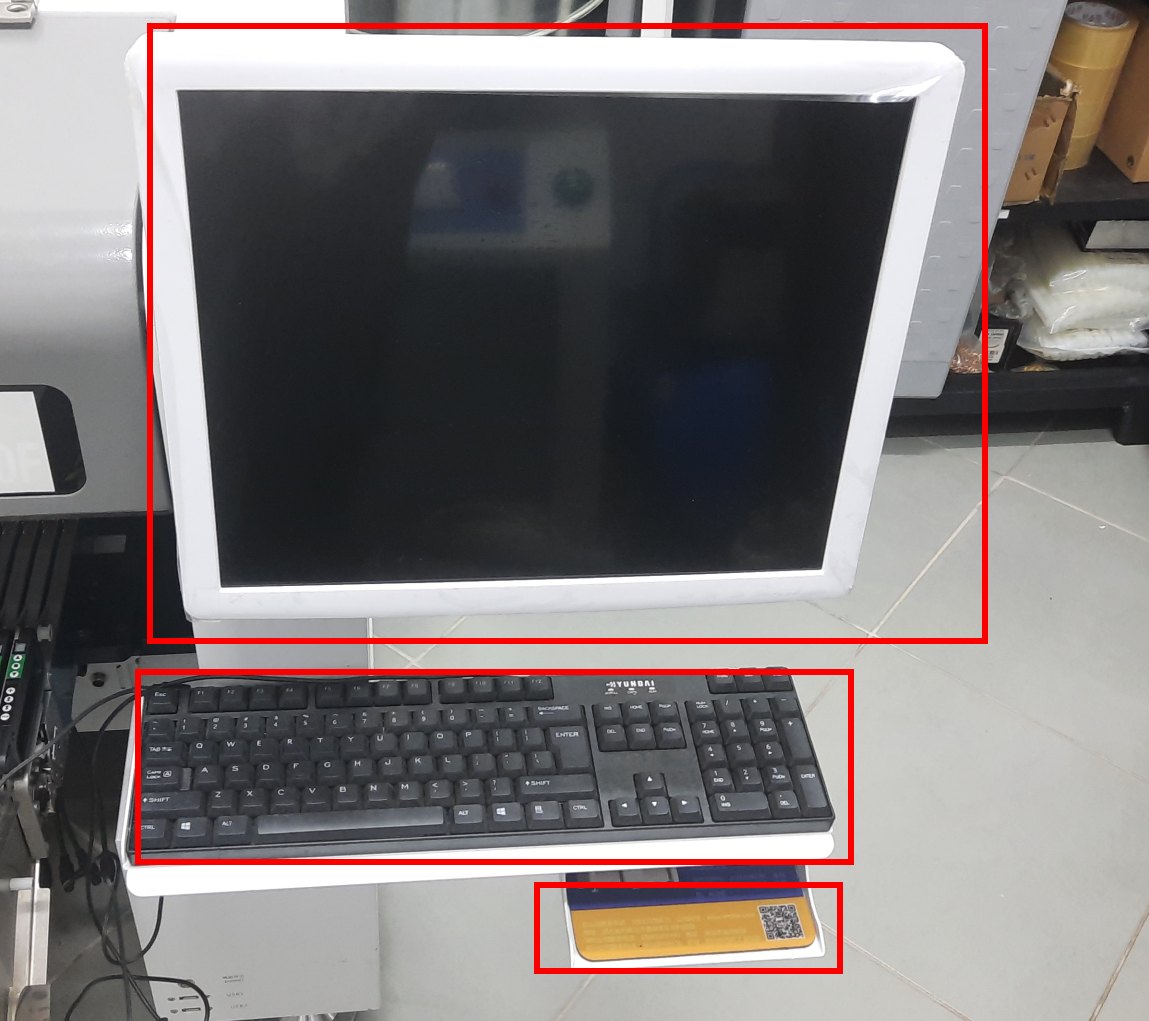
\includegraphics[width=.6\textwidth]{images/hmi.png}
 \caption{HW-T4-50F's human machine interface}
 \end{figure}
 \begin{figure}[!htb]
 \centering
 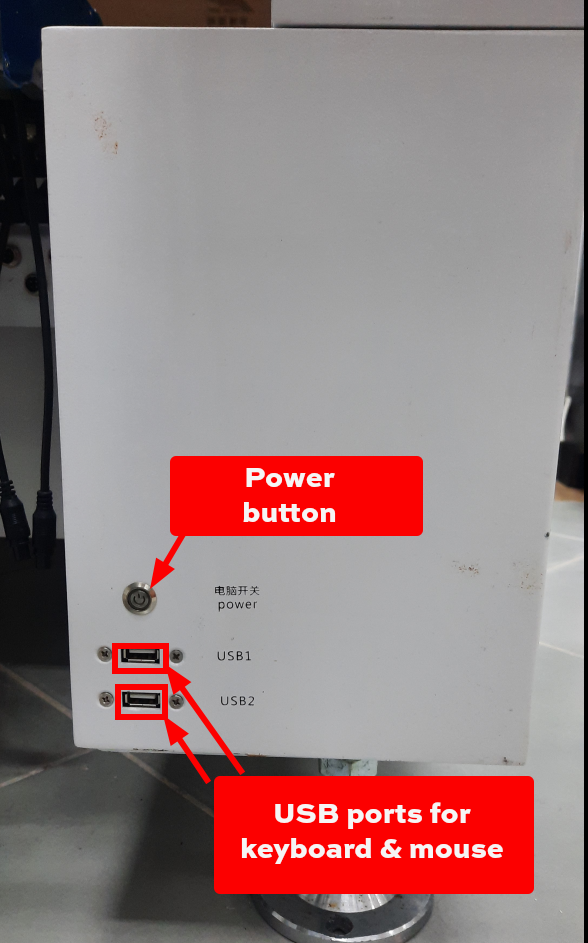
\includegraphics[width=.5\textwidth]{images/computer.png}
 \caption{HW-T4-50F's central computer}
 \end{figure}

\newpage
\section{Introduction to the software}
The HW-T4-50F comes shipped with a graphical user interface that can be used to configure and operate the machine. The user interface contains camera controls, arm controls and pick up head controls. As well as a live camera view.
\begin{figure}[!htb]
 \centering
 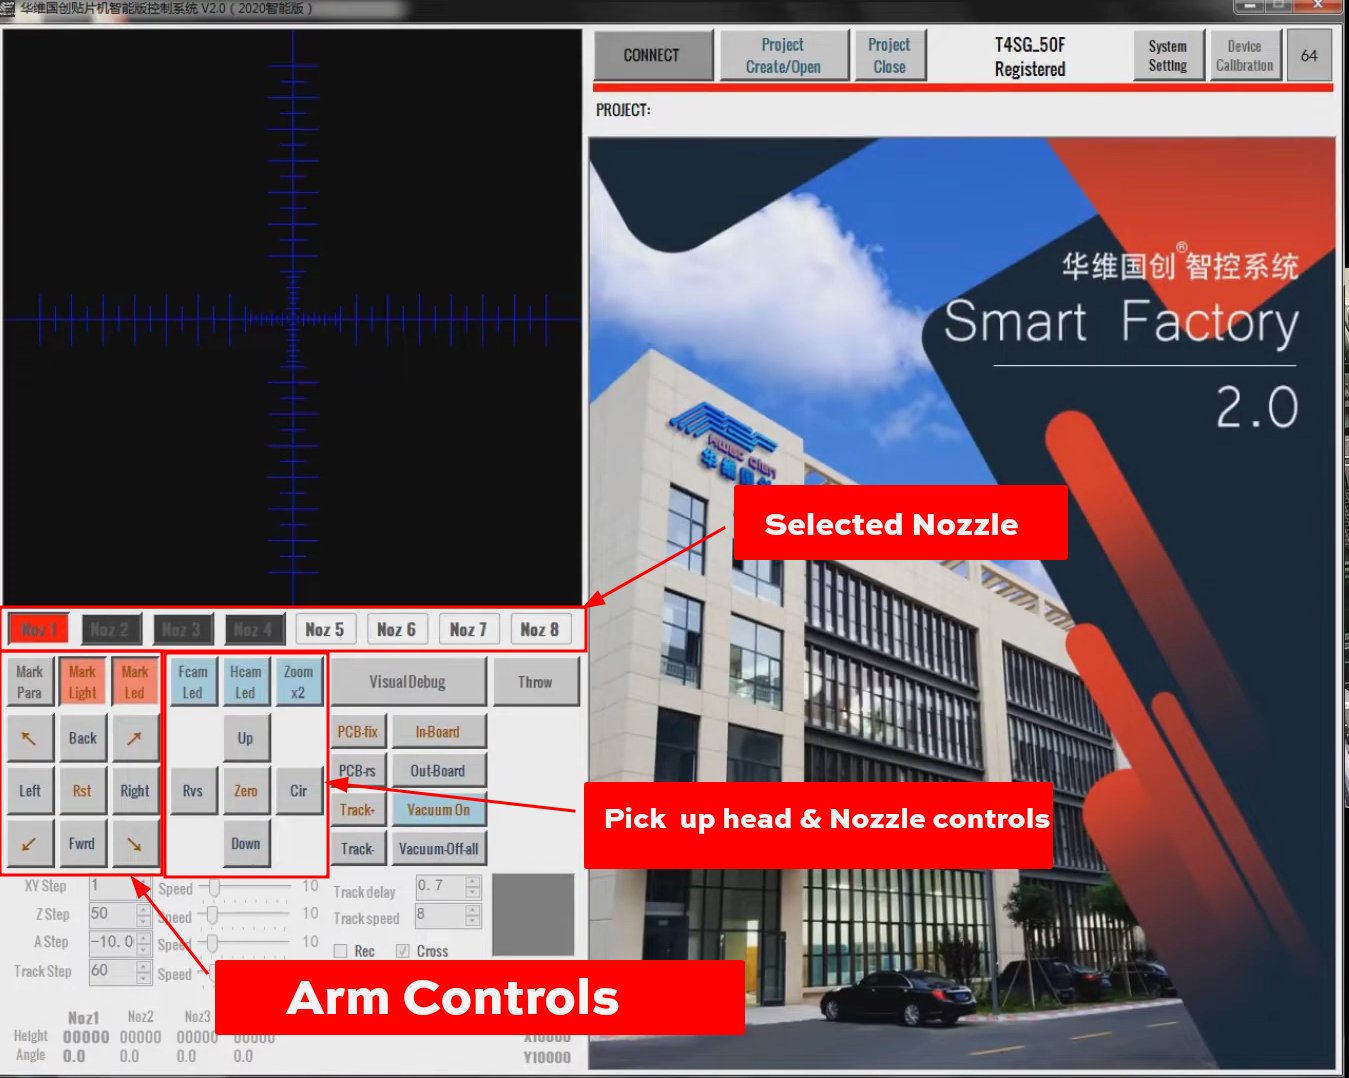
\includegraphics[width=1\textwidth]{images/scrot1.png}
 \caption{A tour of the software}
\end{figure}
\newpage
\section{Registration and software updates}
A user must register the software using the unique ID on the machine's body in order to update to the latest version.
\begin{figure}[!htb]
 \centering
 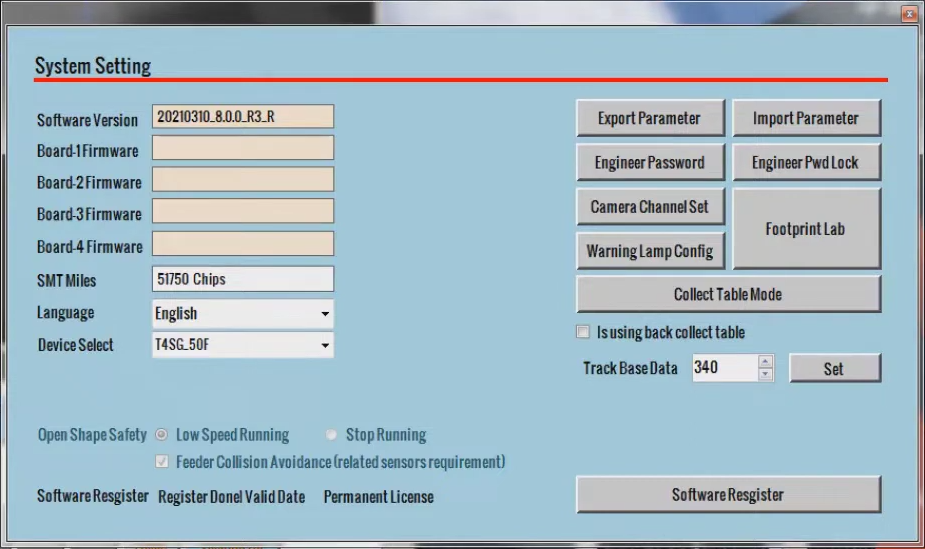
\includegraphics[width=0.8\textwidth]{images/scrot2.png}
 \caption{Software registration and configuration window}
\end{figure}

\section{Pick and Place modes}
The software supports two modes:
\begin{itemize}
 \item \textbf{Manual: } where the user manually picks where components are placed.
 \item \textbf{Automatic: } where the user provides the machine with a pick and place file (usually a CSV file) and lets the machine automatically determine component placement after a calibration process.
\end{itemize}
\begin{figure}[!htb]
 \centering
 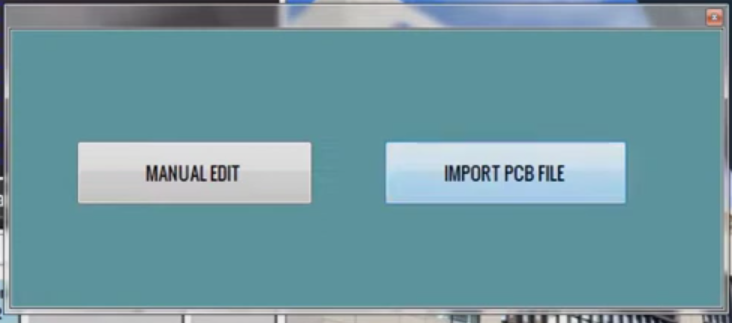
\includegraphics[width=0.8\textwidth]{images/scrot3.png}
 \caption{Software registration and configuration window}
\end{figure}
\textbf{Note: } even if the dialog says "PCB file" the software only takes pick and place files.
\newpage
\section{Pick and place files}
When a pick and place file is imported, all of its columns are \textbf{Unassigned}, the user must manually asign each one.\\

\begin{figure}[!htb]
 \centering
 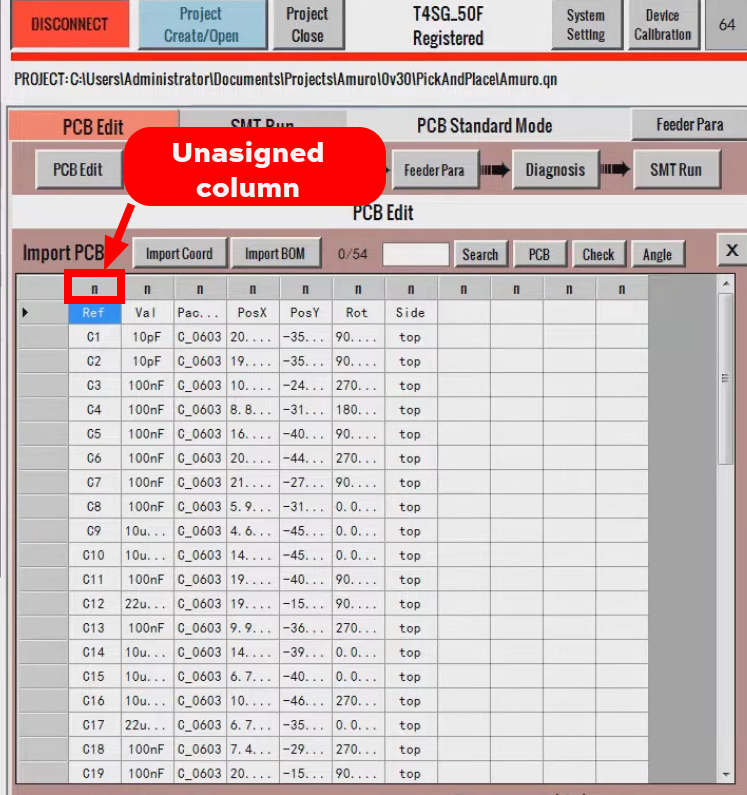
\includegraphics[width=1\textwidth]{images/scrot4_1.png}
 \caption{Unassigned pick and place file}
\end{figure}
Right clicking on the column shows a context menu, selecting an option will assign it to the column
\begin{figure}[!htb]
 \centering
 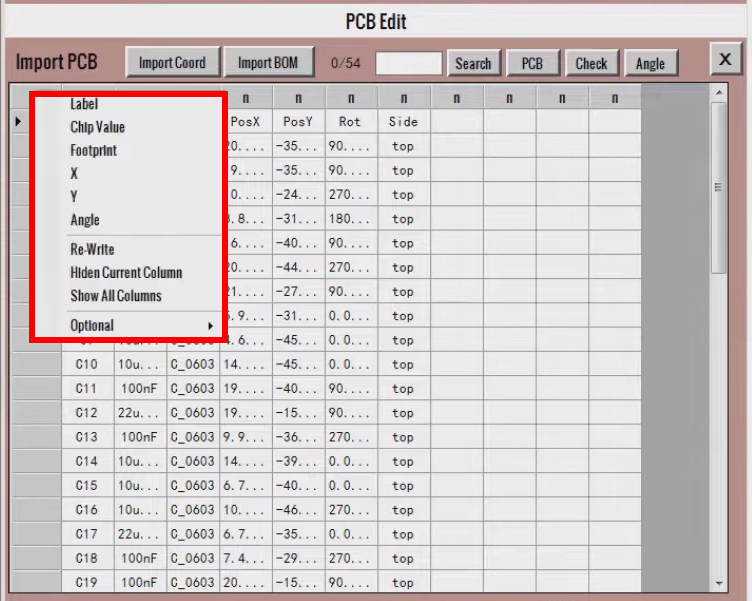
\includegraphics[width=1\textwidth]{images/scrot4_2.png}
 \caption{Unassigned pick and place file}
\end{figure}
\newpage
Essential columns that must be assigned before any pick and place operation are:
\begin{itemize}
 \item \textbf{Label}
 \item \textbf{Chip Value}
 \item \textbf{Footprint}
 \item \textbf{X coordinate}
 \item \textbf{Y coordinate}
 \item \textbf{Rotation angle}
\end{itemize}
These columns are strictly required, but there are other optional columns such as \textbf{Layer} etc...\\
\textbf{Important note: } The user must delete any row that doesn't contain valid component information, including logo and fiducial marks.\\
\newpage
\section{Fiducial marks and calibration}
\subsection{Calibrating a PCB}
The caliration of the pick and place machine starts at the pcb design, designers must include fiducial mark that will help the machine calibrate its coordinate system to the board.\\

The calibration process starts by picking the fiducial marks from the pick and place table, the user may only use 2 marks, but 4 are recommended for improved precision. By default only 2 marks are available, the user may change them to 4 by checking the \textbf{"Precise mode"} box\\

To choose a fiducial mark the user must right click on the appropriate row and click "set as Sign" from the context menu. Sign is just another word for fiducial mark and each PCB has 4 signs (in precise mode). Signs are picked in order and according to the PCB's orientation.\\

\textbf{Note:} for PCB Arrays, the user only needs to load the pick and place files of a single pcb.
\begin{figure}[!htb]
 \centering
 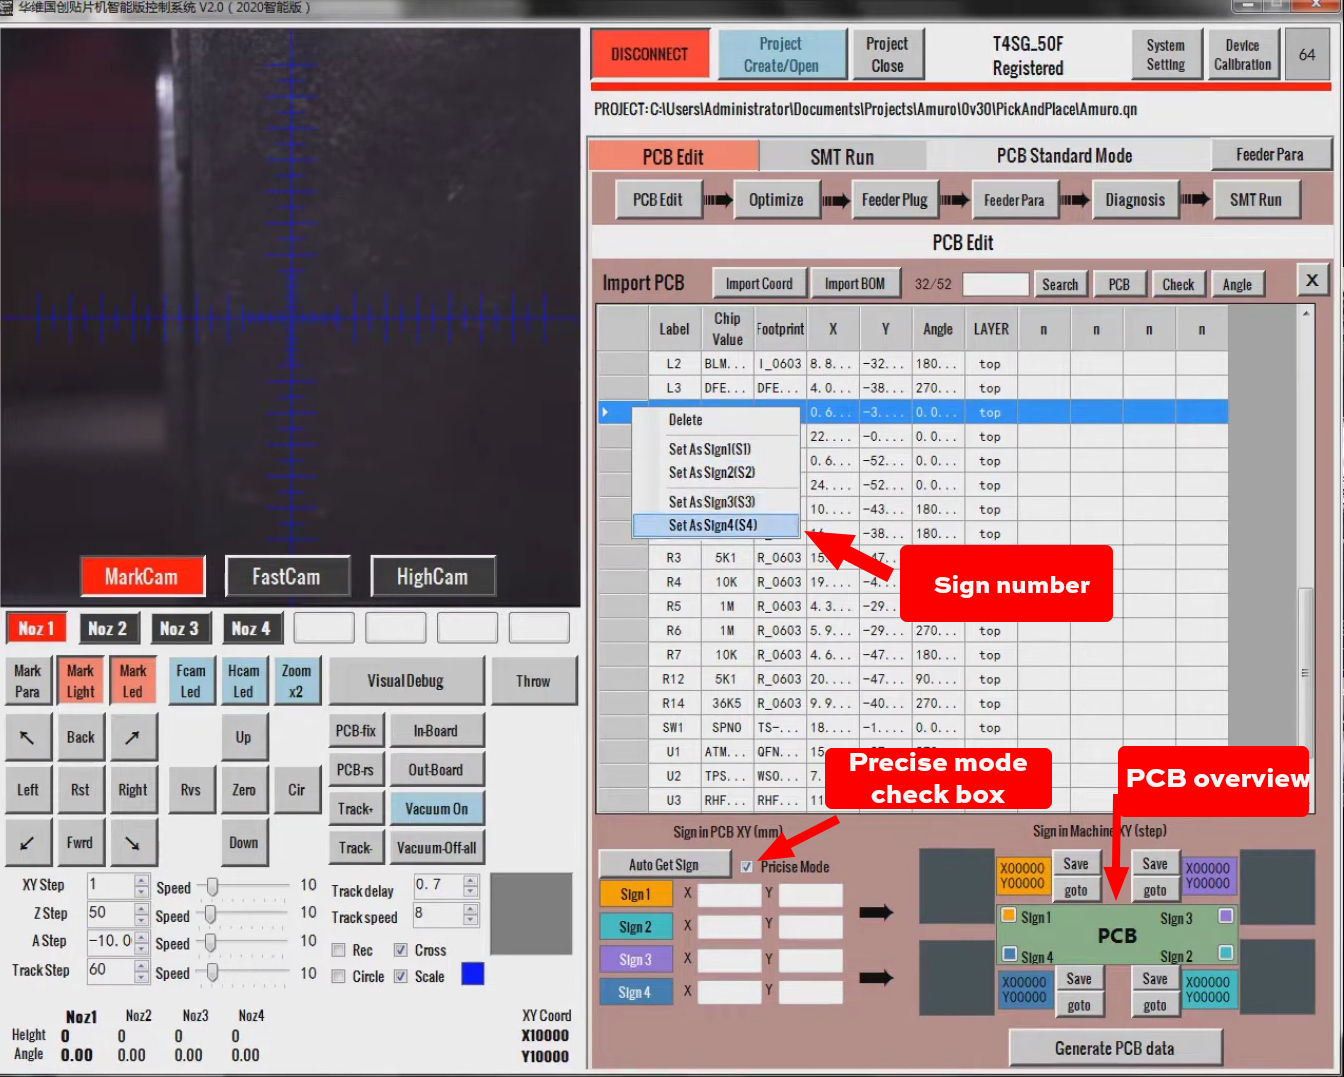
\includegraphics[width=1\textwidth]{images/scrot5.png}
 \caption{Fiducial marks from the pick and place table}
\end{figure}

\newpage
After pointing the \textbf{Mark Cam} at a fiducial mark, using the directional arrows, the user must click \textbf{"Save"} in order to save its coordinates.

Clicking on \textbf{"goto"} will displace the camera to a saved mark.\\
\begin{figure}[!htb]
 \centering
 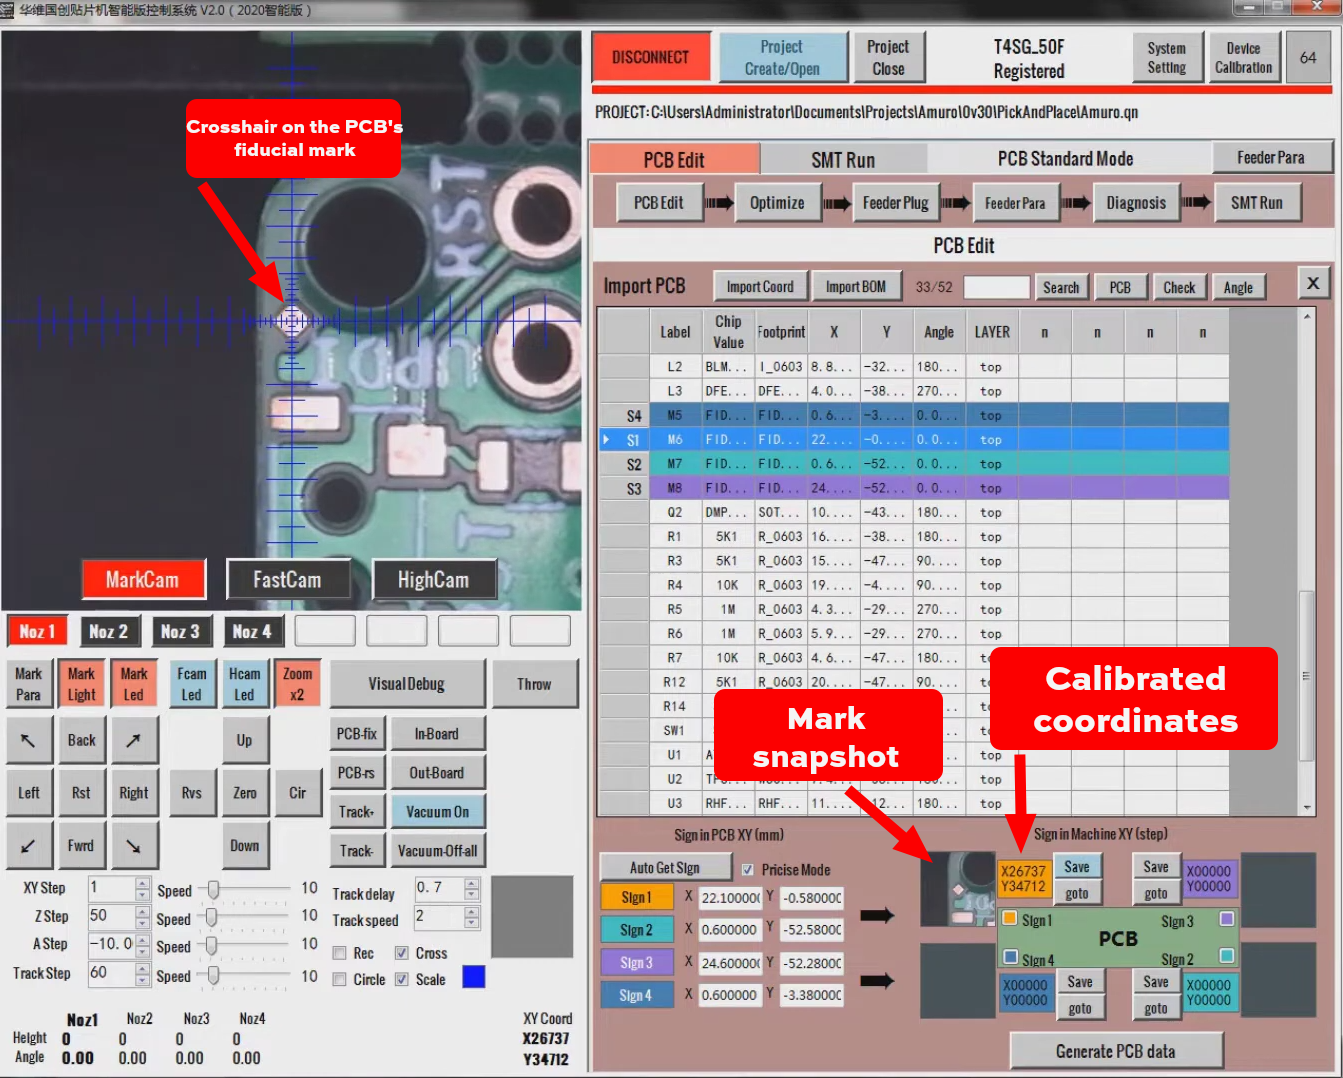
\includegraphics[width=1\textwidth]{images/scrot6.png}
 \caption{First fiducial mark calibration}
\end{figure}
\newpage
The last step is clicking on the "Generate PCB Data" button to create a table of traversable points in the PCB on which components will be placed. The "Goto" buttons are useful for traversing each point and verifying the accuracy of the calibration.\\

\begin{figure}[!htb]
 \centering
 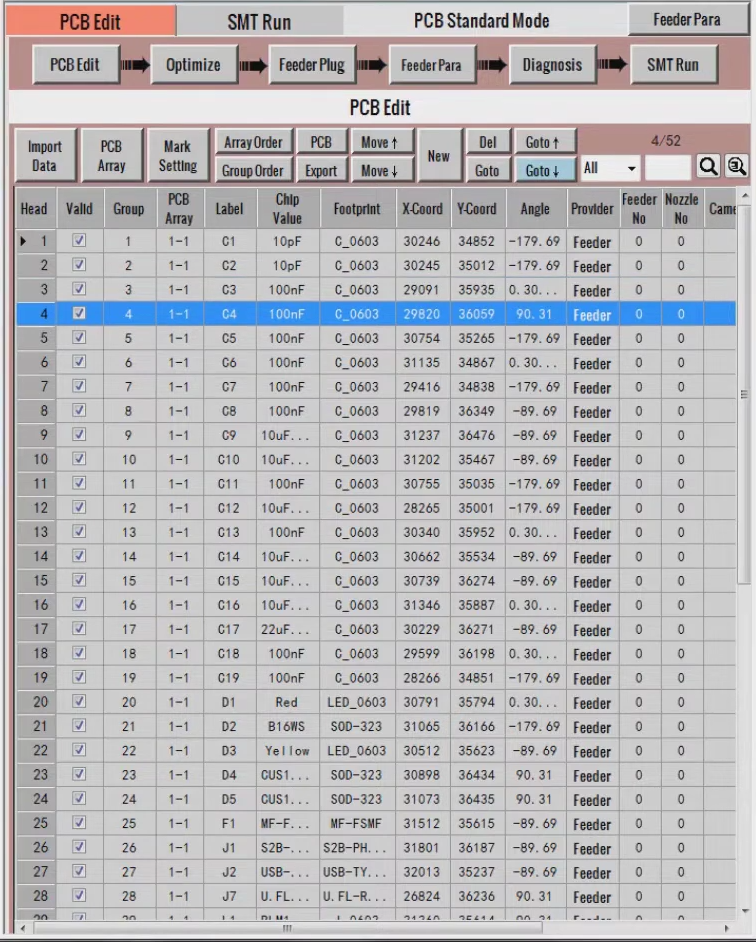
\includegraphics[width=1\textwidth]{images/scrot7_1.png}
 \caption{Generated PCB data}
\end{figure}
\textbf{Note:} For Single PCB designs, steps in \textbf{\textbf{\hyperref[sec:1.9.2]{images/section 1.9.2}} and \textbf{\hyperref[sec:1.9.4]{images/section 1.9.4}}} can be skipped.
\newpage
\subsection{Calibrating coupled PCB arrays}
\label{sec:1.9.2}
The HW-T4-50F can be configured to handle PCB Arrays (also called \textbf{Panels}) with relative ease.\\

After following the instructions in the \textbf{previous section}, the user must click the \textbf{"PCB Array"} button to begin the PCB Array calibration process.
\begin{figure}[!htb]
 \centering
 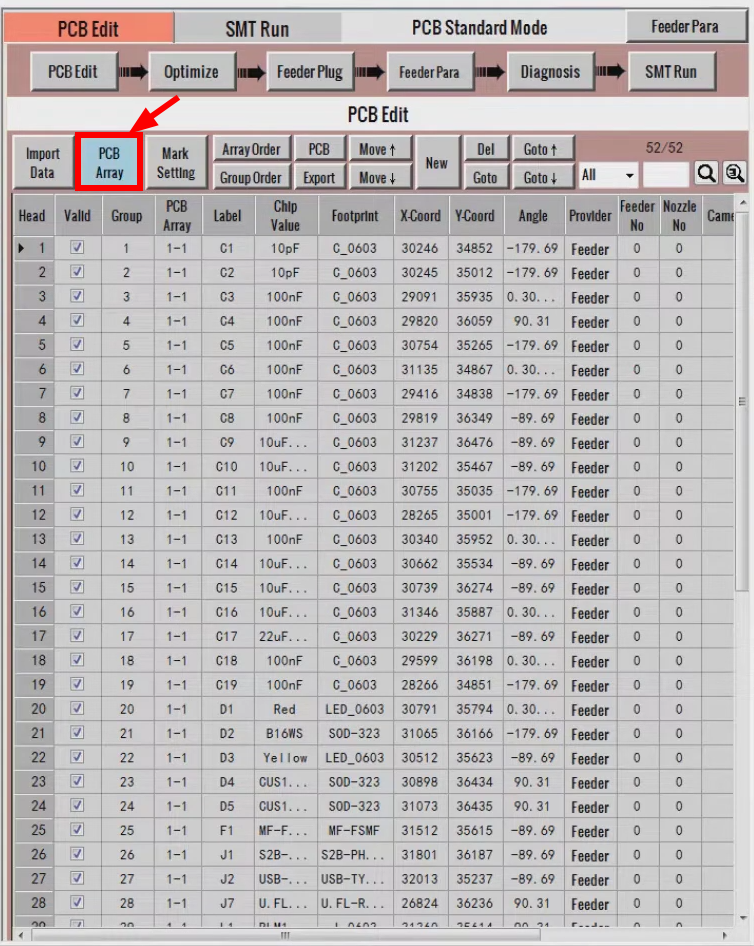
\includegraphics[width=0.9\textwidth]{images/scrot7.png}
 \caption{PCB array button on the generated PCB data window}
\end{figure}
\newpage

To begin calibrating a coupled PCB layout, check the \textbf{"CouplePCB"} box.\\
\begin{figure}[!htb]
 \centering
 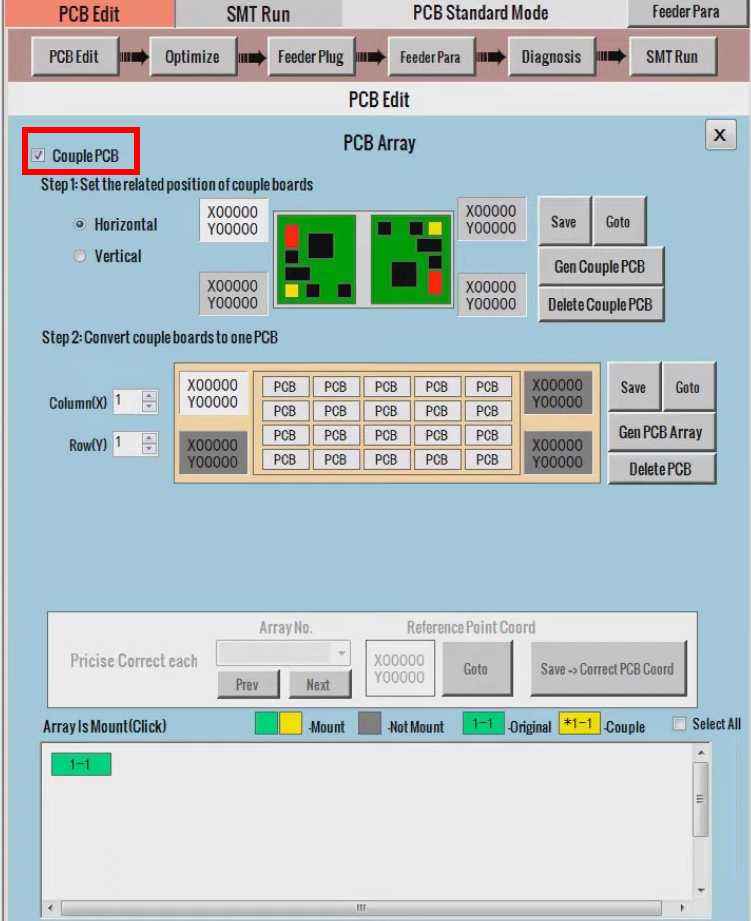
\includegraphics[width=1\textwidth]{images/scrot8.png}
 \caption{PCB array button on the generated PCB data window}
\end{figure}
\newpage
Select homologous points from the PCBs as specified in the drawing.\\
To calibrate a row (or a column in a horizontally mirrored couple PCB).
After Calibrating, click \textbf{"Generate Couple PCB"}.
\begin{figure}[!htb]
 \centering
 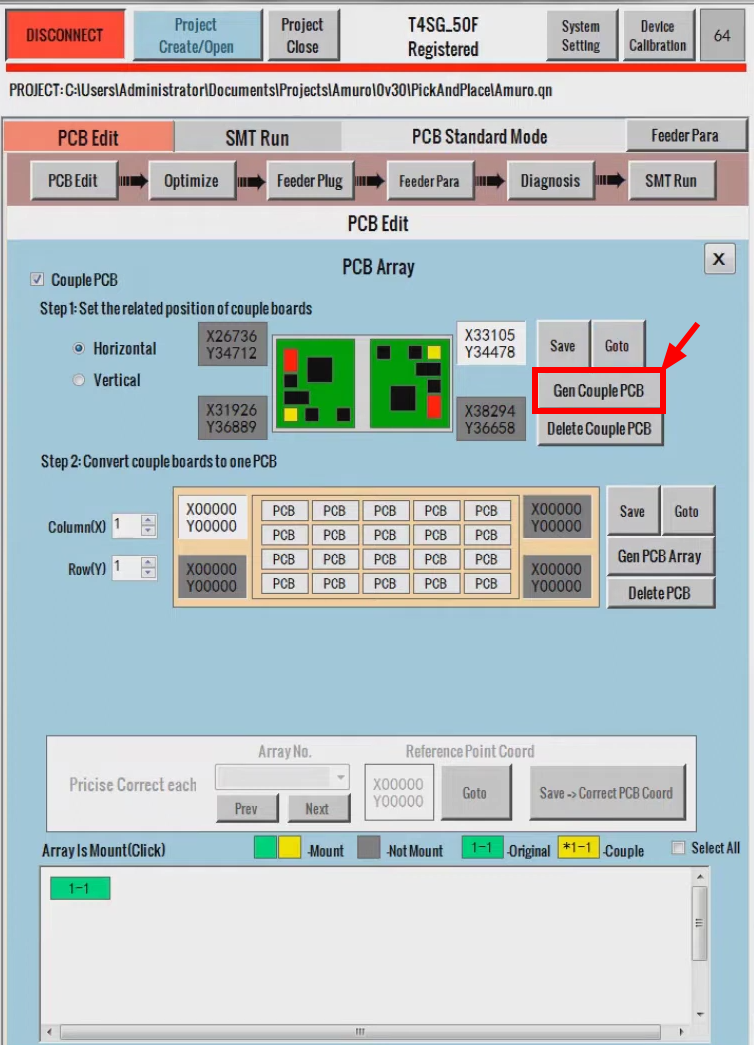
\includegraphics[width=0.9\textwidth]{images/scrot9.png}
 \caption{Generating a coupled PCB}
\end{figure}

\newpage
In this example, the generated couple is a full row (with two columns). The number of rows / columns is configured via the corresponding textboxes.\\

\begin{figure}[!htb]
 \centering
 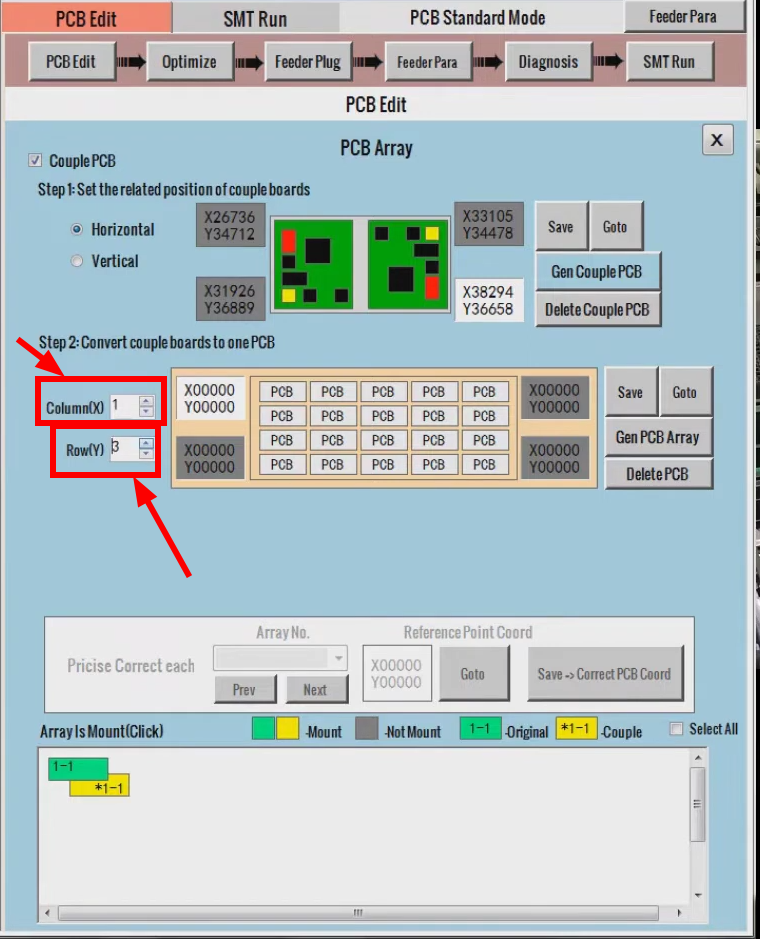
\includegraphics[width=1\textwidth]{images/scrot10.png}
 \caption{Column / Row count textboxes}
\end{figure}
After selecting the PCB array's edges the software will generate the rest of the array automatically.
\newpage
\subsection{Working with non coupled PCB arrays}
PCB arrays shaped other than 2xN or Nx2 (Non coupled), require extra attention from the user.\\

In this section, we will work on a 3x4 pcb array. But the same steps apply to any other array shape.\\
The user must calibrate the pick and place machine using the four corner PCBs of the PCB array .\\ Corner marks are fiducial marks selected from
corner PCBs.
The sole criteria for corner mark selection is that selected fiducial marks must remain consistent across all four PCBs (\textbf{e.g:} If the user selects fiducial mark 1 on the first corner PCB, they must use fiducial mark 1 for the remaining 3) .\\
Consider the following PCB array:

\begin{figure}[!htb]
 \centering
 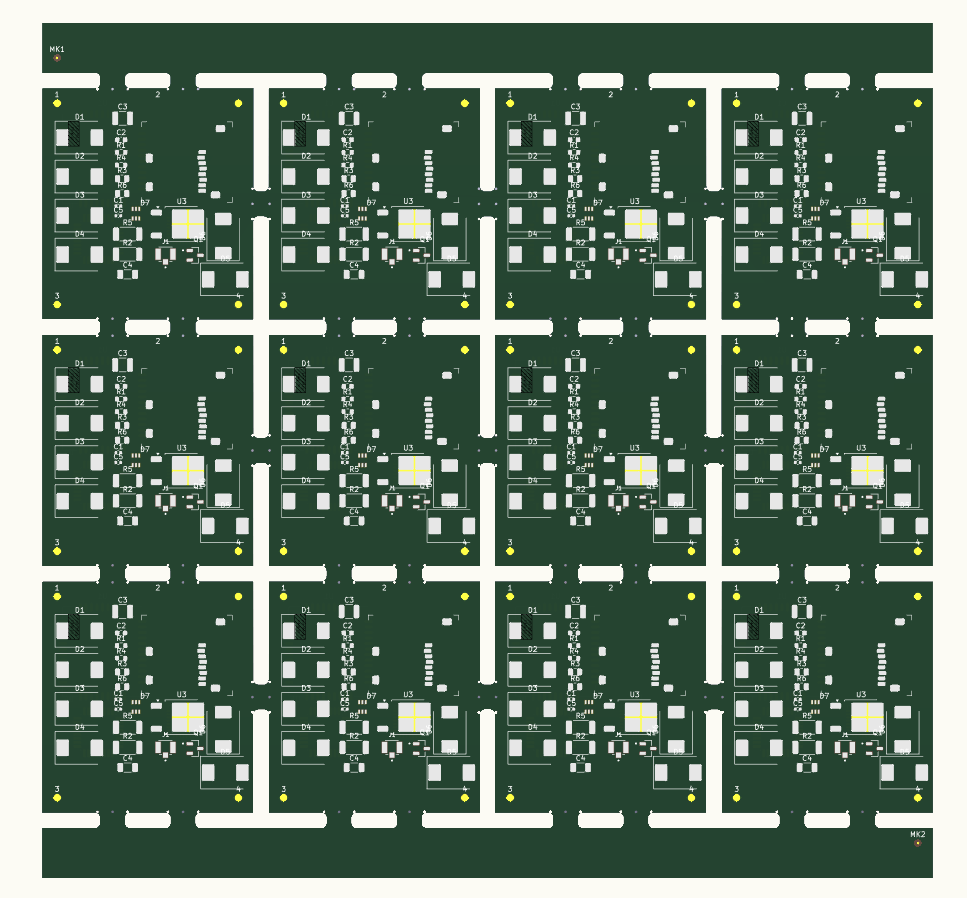
\includegraphics[width=1\textwidth]{images/panel_mini_a4.png}
 \caption{Example 3x4 PCB array}
\end{figure}

In order to calibrate the machine, the user must select consistent fiducial marks across the four corner PCBs.
\newpage
\begin{figure}[!htb]
 \centering
 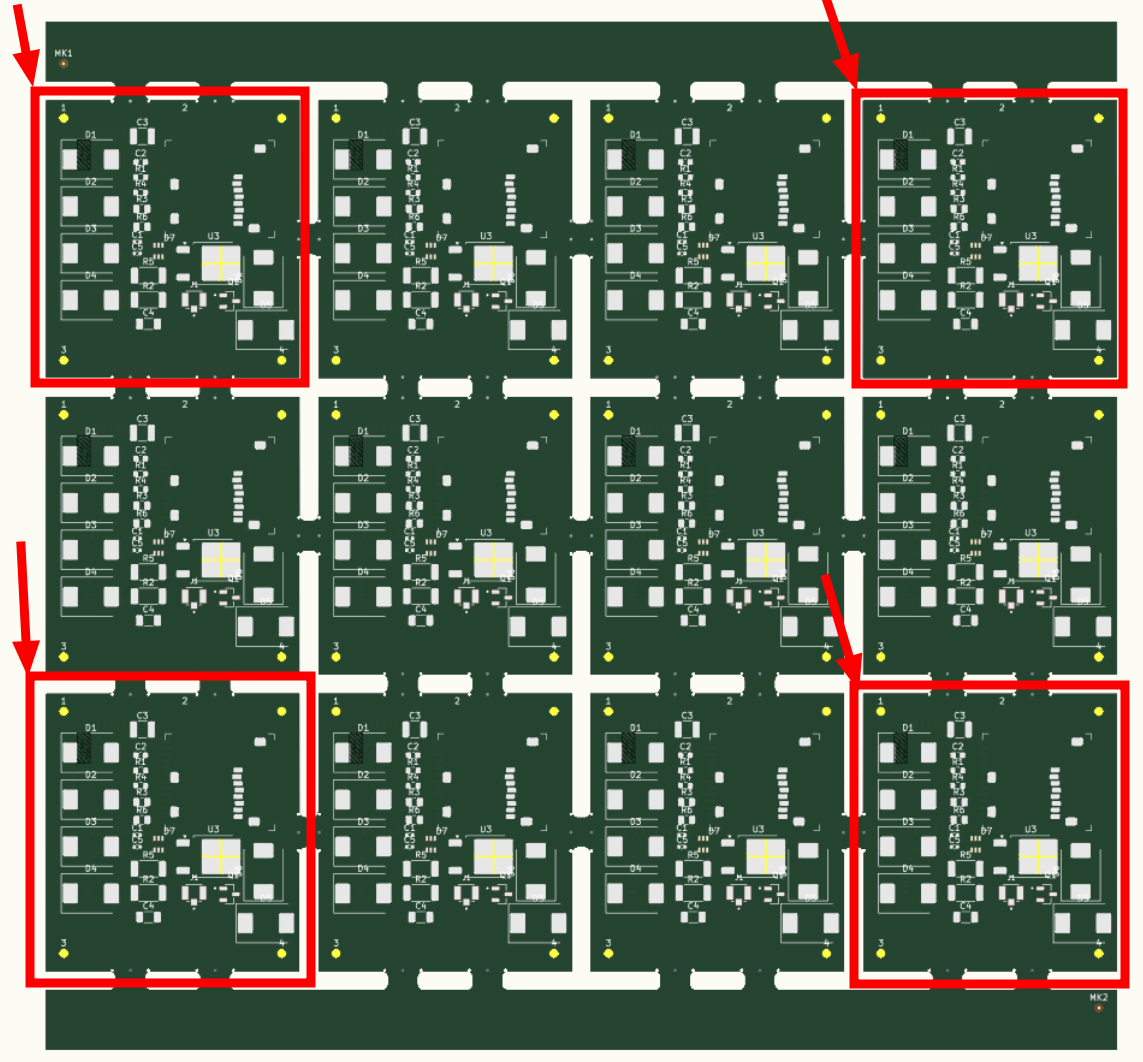
\includegraphics[width=0.65\textwidth]{images/panel_mini_a4_corners.png}
 \caption{Corner PCBs}
\end{figure}
\begin{figure}[!htb]
 \centering
 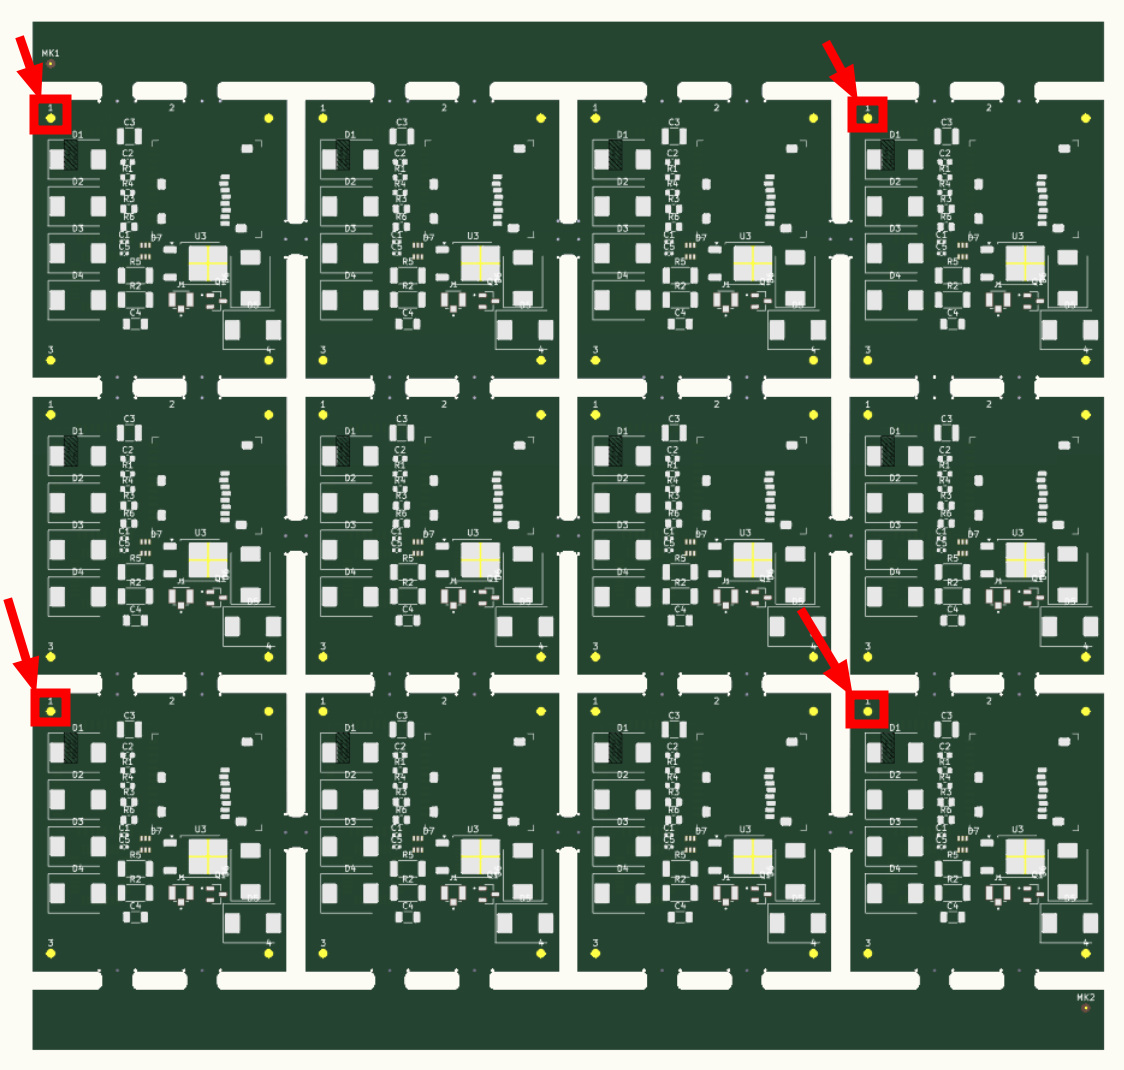
\includegraphics[width=0.65\textwidth]{images/panel_mini_a4_marks.png}
 \caption{Example corner marks}
\end{figure}
\newpage
After pointing the \textbf{Mark Cam} at the selected point, the user must select the corresponding corner on the PCB Array configuration panel and hit the \textbf{"save"} button.
\begin{figure}[!htb]
 \centering
 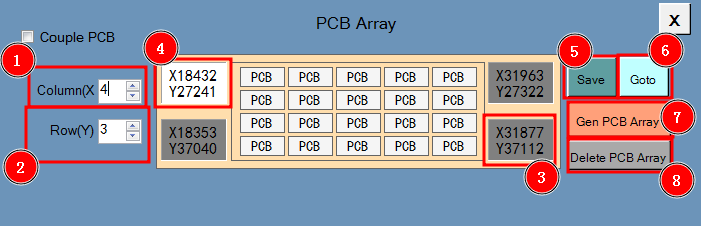
\includegraphics[width=1\textwidth]{images/scrot11.png}
 \caption{PCB Edit tab: Corner mark calibration}
\end{figure}
\begin{itemize}
 \item \textbf{1: } Column count
 \item \textbf{2: } Row count
 \item \textbf{3: } Saved corner coordinates
 \item \textbf{4: } Selected corner
 \item \textbf{5: } Save \textbf{Mark Cam} coordinates to selected corner
 \item \textbf{6: } Move \textbf{Mark Cam} to selected corner coordinates
 \item \textbf{7: } Generate PCB array
 \item \textbf{8: } Delete current PCB array.
\end{itemize}

Once the user has picked the four corner coordinates, the PCB Array can be generated by clicking the \textbf{"Gen PCB Array"} button.\\
\newpage
Once generated, PCBs on the PCB array should be automatically recognized as \textbf{Cells} of the array. On the \textbf{PCB Edit} tab the user can also  browse and adjust the array cells: \\

\begin{figure}[!htb]
 \centering
 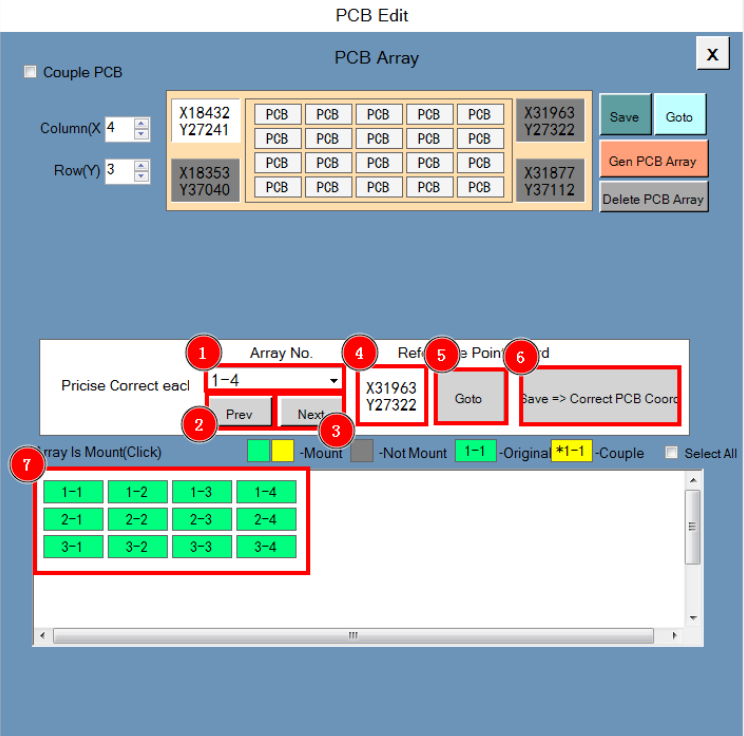
\includegraphics[width=1\textwidth]{images/scrot14.png}
 \caption{PCB Edit tab: PCB array verification}
\end{figure}
\begin{itemize}
 \item \textbf{1: } Selected cell
 \item \textbf{2: } Previous cell
 \item \textbf{3: } Next cell
 \item \textbf{4: } Cell mark coordinates
 \item \textbf{5: } Move \textbf{Mark Cam} to cell mark
 \item \textbf{6: } Save \textbf{Mark Cam} coordinates to cell mark
 \item \textbf{7: } PCB array overview
\end{itemize}
\newpage
\subsection{Mark calibration}
\label{sec:1.9.4}
After going through the previous steps the user must configure panel marks. Panel Marks are fiducial marks found on the PCB Panel rails.\\

Panel marks are also called \textbf{global fiducial marks} as opposed to local fiducial marks that are found on the individual PCBs which we used to calibrate the machine in \textbf{\hyperref[sec:1.9.2]{images/section 1.9.2}}.\\
Clicking on the \textbf{"Mark Setting"} button will open the Panel Mark calibration menu.\\

\begin{figure}[!htb]
 \centering
 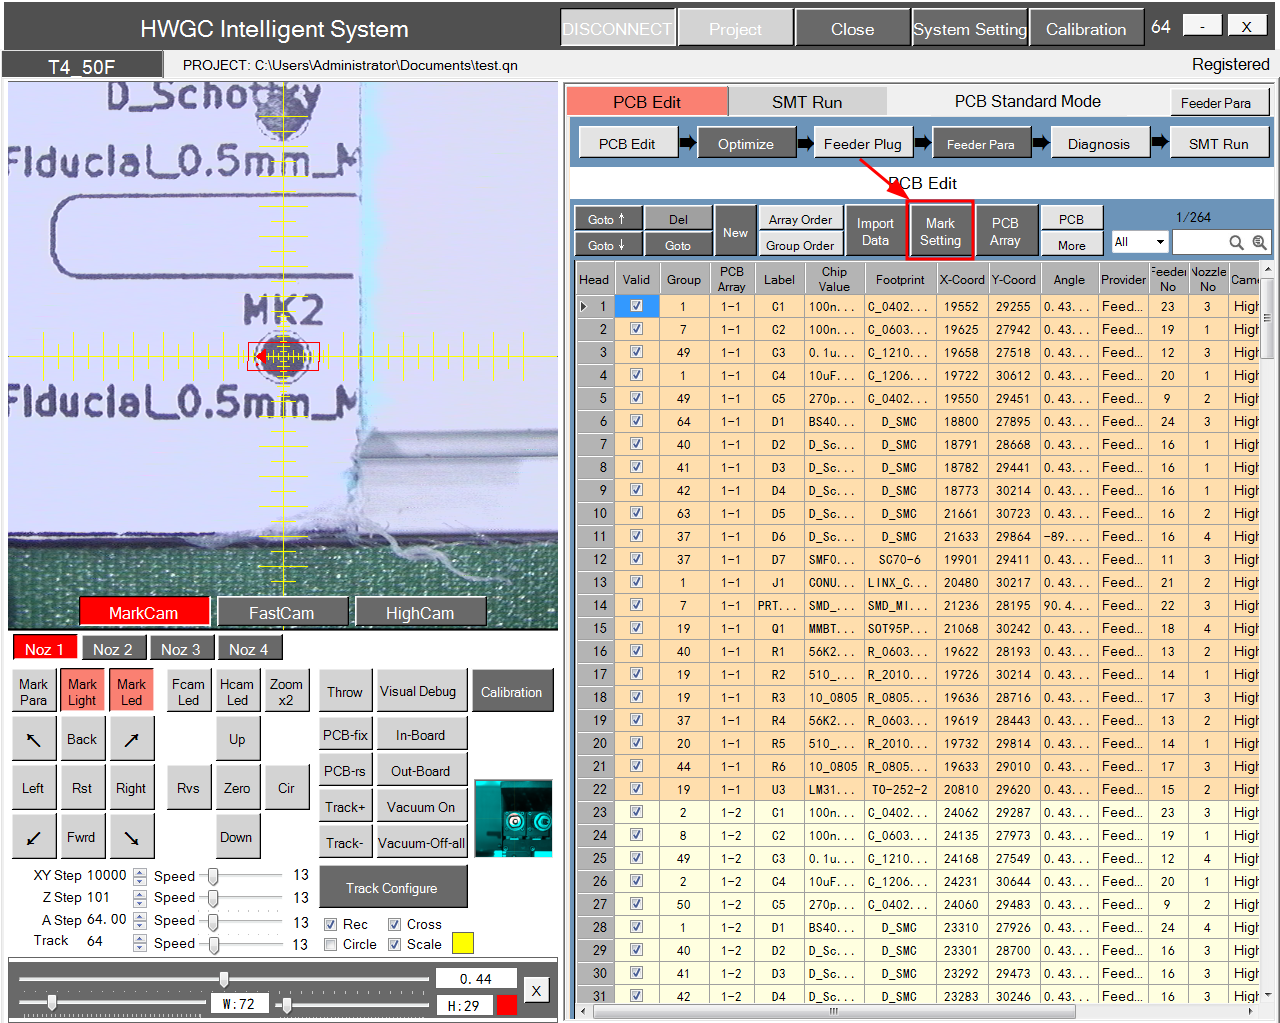
\includegraphics[width=1\textwidth]{images/scrot16.png}
 \caption{PCB Edit tab: Mark Setting button}
\end{figure}
\newpage
Following the same logic as local fiducial mark calibration, the user must point the \textbf{Mark Cam} at the two fiducial marks on the PCB Panel rails. The marks must be on opposite ends of each other.
\begin{figure}[!htb]
 \centering
 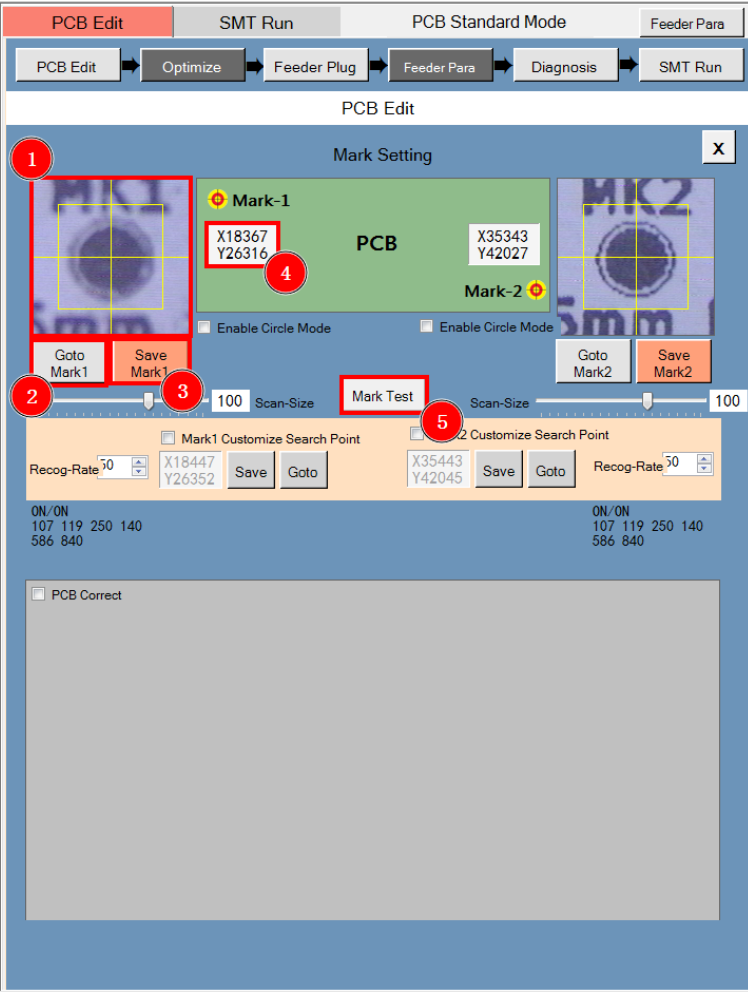
\includegraphics[width=0.75\textwidth]{images/scrot17.png}
 \caption{PCB Edit tab: Panel Mark calibration}
\end{figure}
\begin{itemize}
 \item \textbf{1: } Mark snapshot
 \item \textbf{2: } Go to mark
 \item \textbf{3: } Save \textbf{Mark Cam} coordinates to mark
 \item \textbf{4: } Mark coordinates
 \item \textbf{5: } Initiate Mark test
\end{itemize}

\subsubsection{Mark test}
The \textbf{Mark test} is an automated test that allows the user to verify mark config, this is particularly useful when reloading the project for subsequent use.
\newpage
\section{Feeder setup and calibration}
\subsection{How to setup a tape feeders}
Throughout this section we will be using the \textbf{YMH-EF8-0000} Electric feeder. The pick and place machine sends the same signals to both pneumatic and electric feeders so we don't need to worry about differences between the two.
\begin{figure}[!htb]
 \centering
 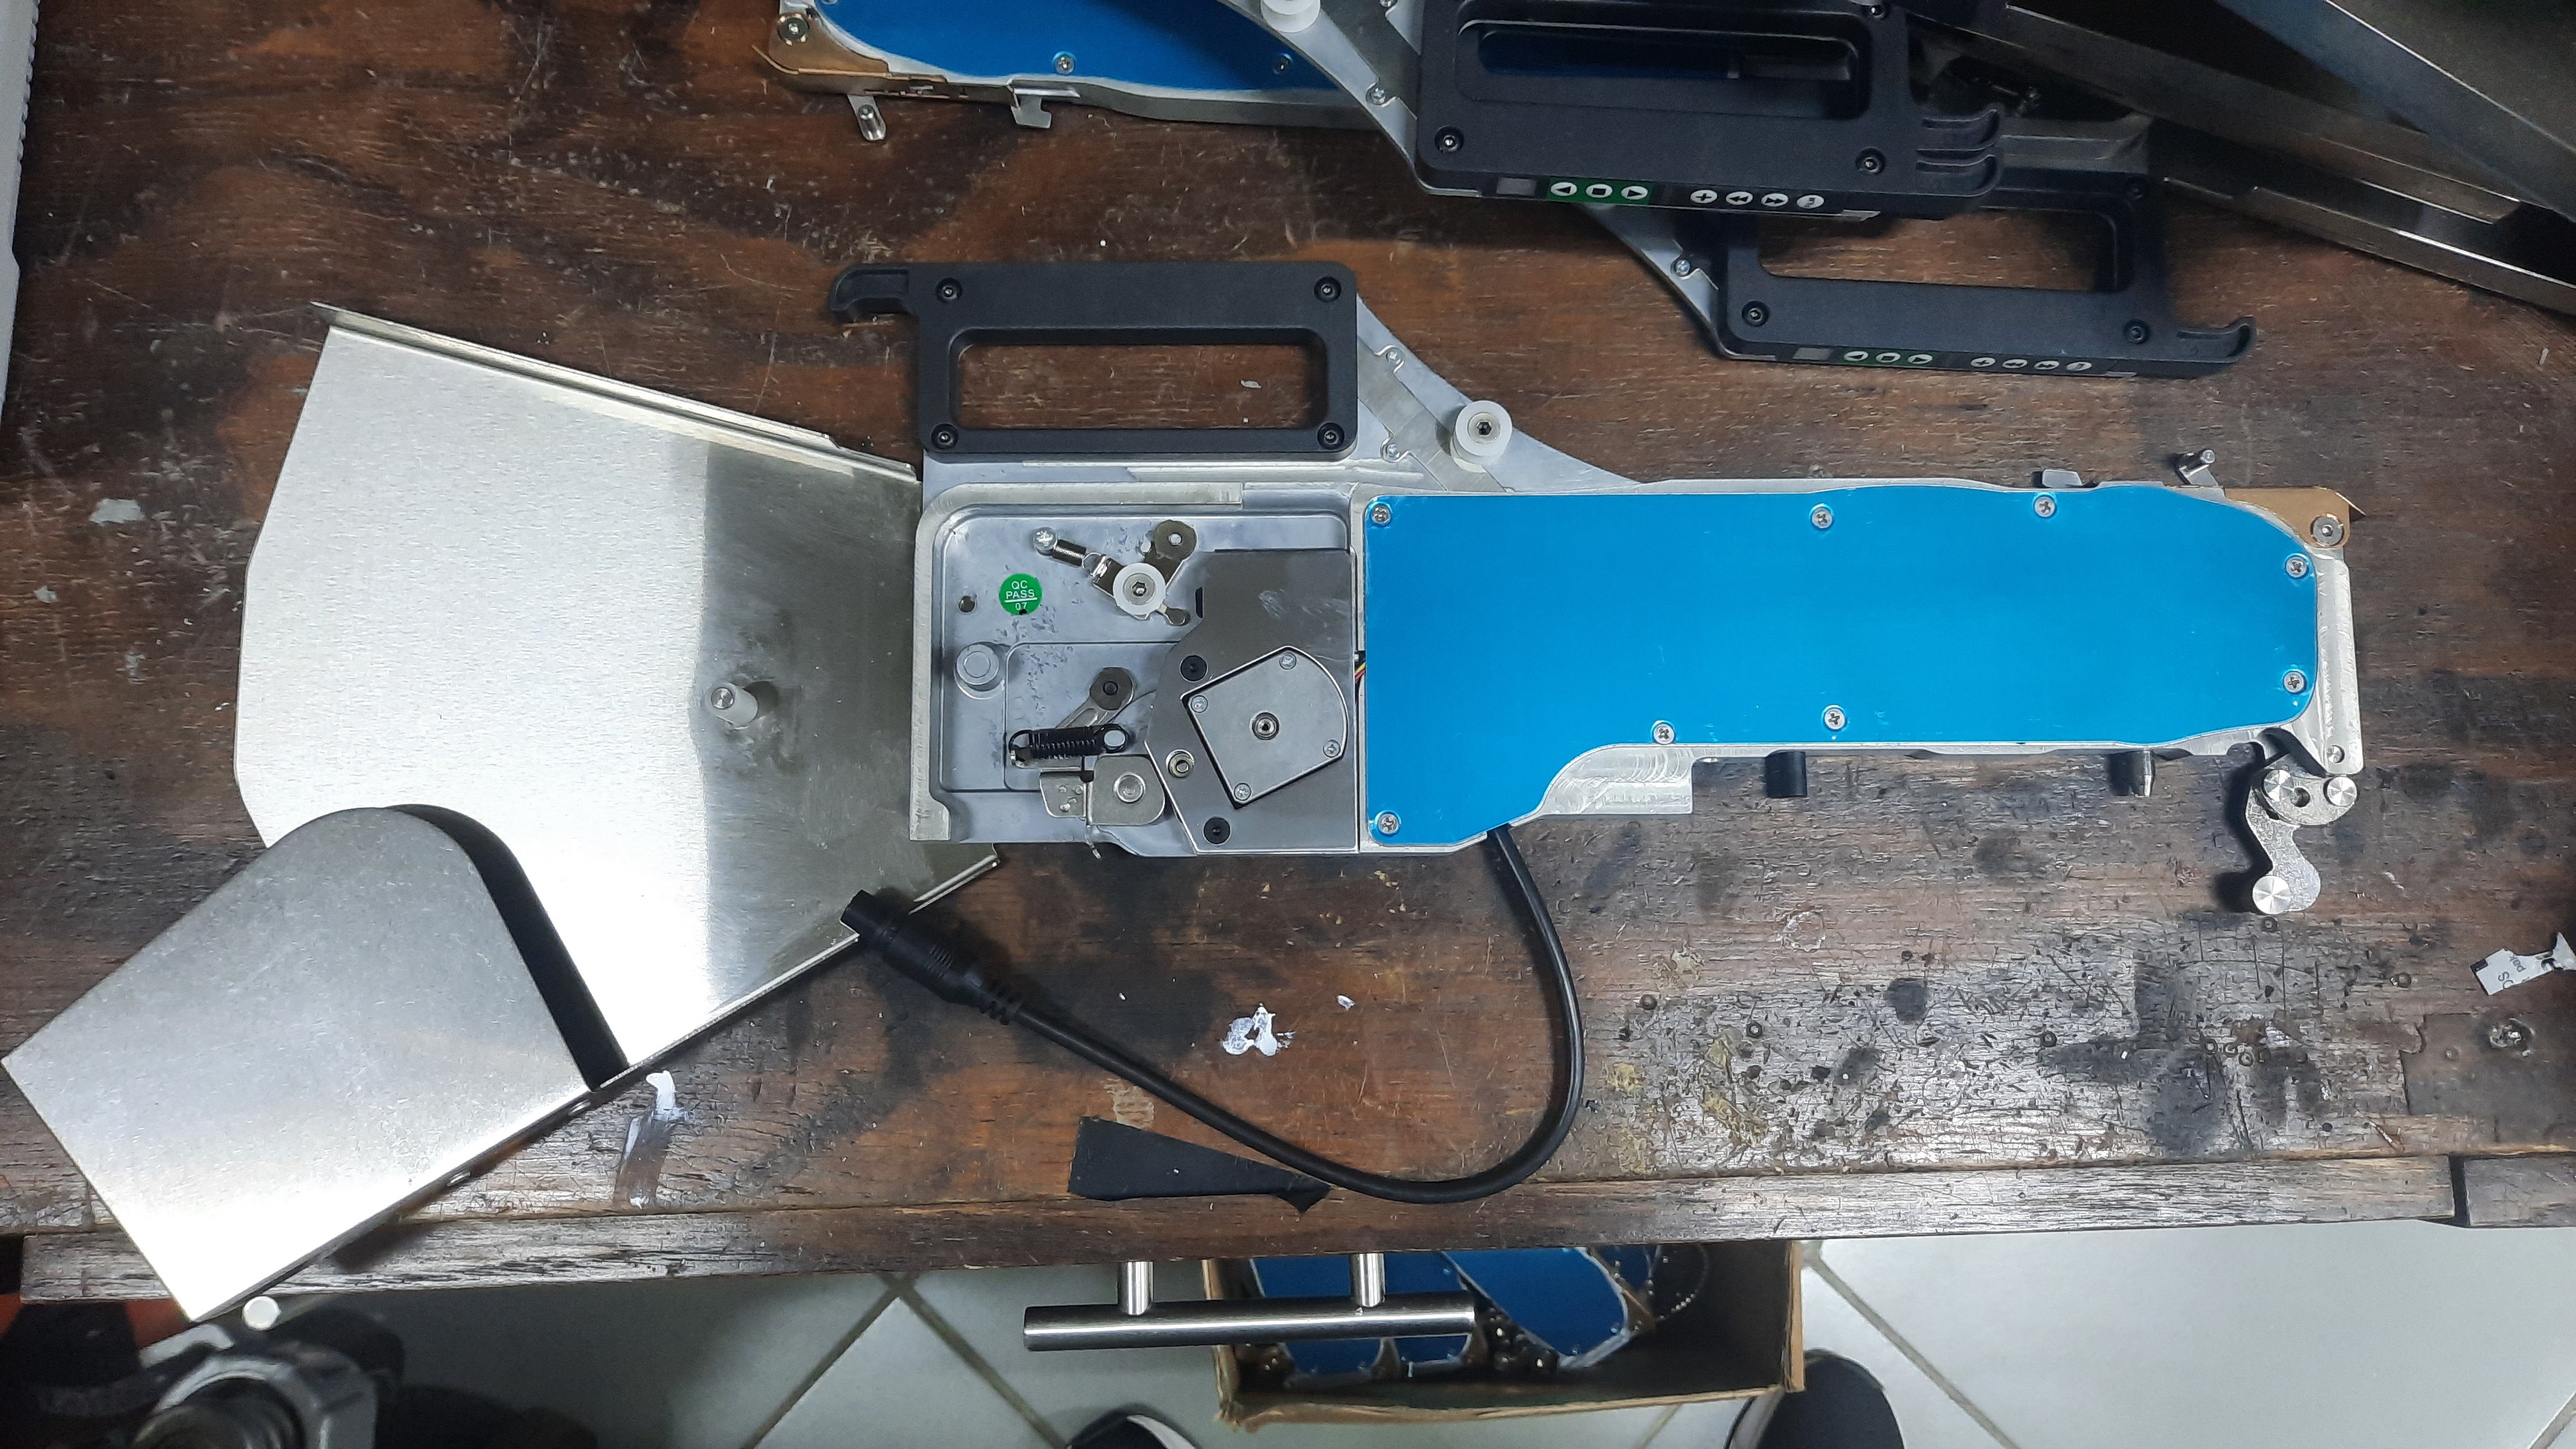
\includegraphics[width=1\textwidth]{images/feeder.jpg}
 \caption{The YMH-EF8-0000}
\end{figure}
\newpage
\subsubsection{Step 1: Choosing the right tape}
Every feeder setup starts with picking the right tape. Our feeder is compatible with 8mm tape. For components that only come in larger tapes, we might have to pick another feeder. Standard tape sizes are:

\begin{itemize}
    \item \textbf{8 mm Tape:} This is the most common size and is typically used for small passive components like resistors, capacitors, and small ICs (Integrated Circuits).
    \item \textbf{12 mm Tape:} Used for slightly larger components such as larger capacitors, ICs, and connectors.
    \item \textbf{16 mm Tape:} Suitable for medium-sized components, including larger ICs and some connectors.
    \item \textbf{24 mm Tape:} Used for even larger components, such as large ICs, connectors, and modules.
    \item \textbf{32 mm Tape:} This size is often used for large connectors, power components, and some mechanical parts.
    \item \textbf{44 mm Tape:} Suitable for very large components and mechanical parts.
    \item \textbf{56 mm Tape:} Used for very large components, modules, and certain mechanical assemblies.
    \item \textbf{72 mm Tape:} For extra-large components and assemblies, though less common in standard pick and place operations.
    \item \textbf{88 mm Tape and above:} These are used for special applications and very large components, and their use is less common.
\end{itemize}
\begin{figure}[!htb]
 \centering
 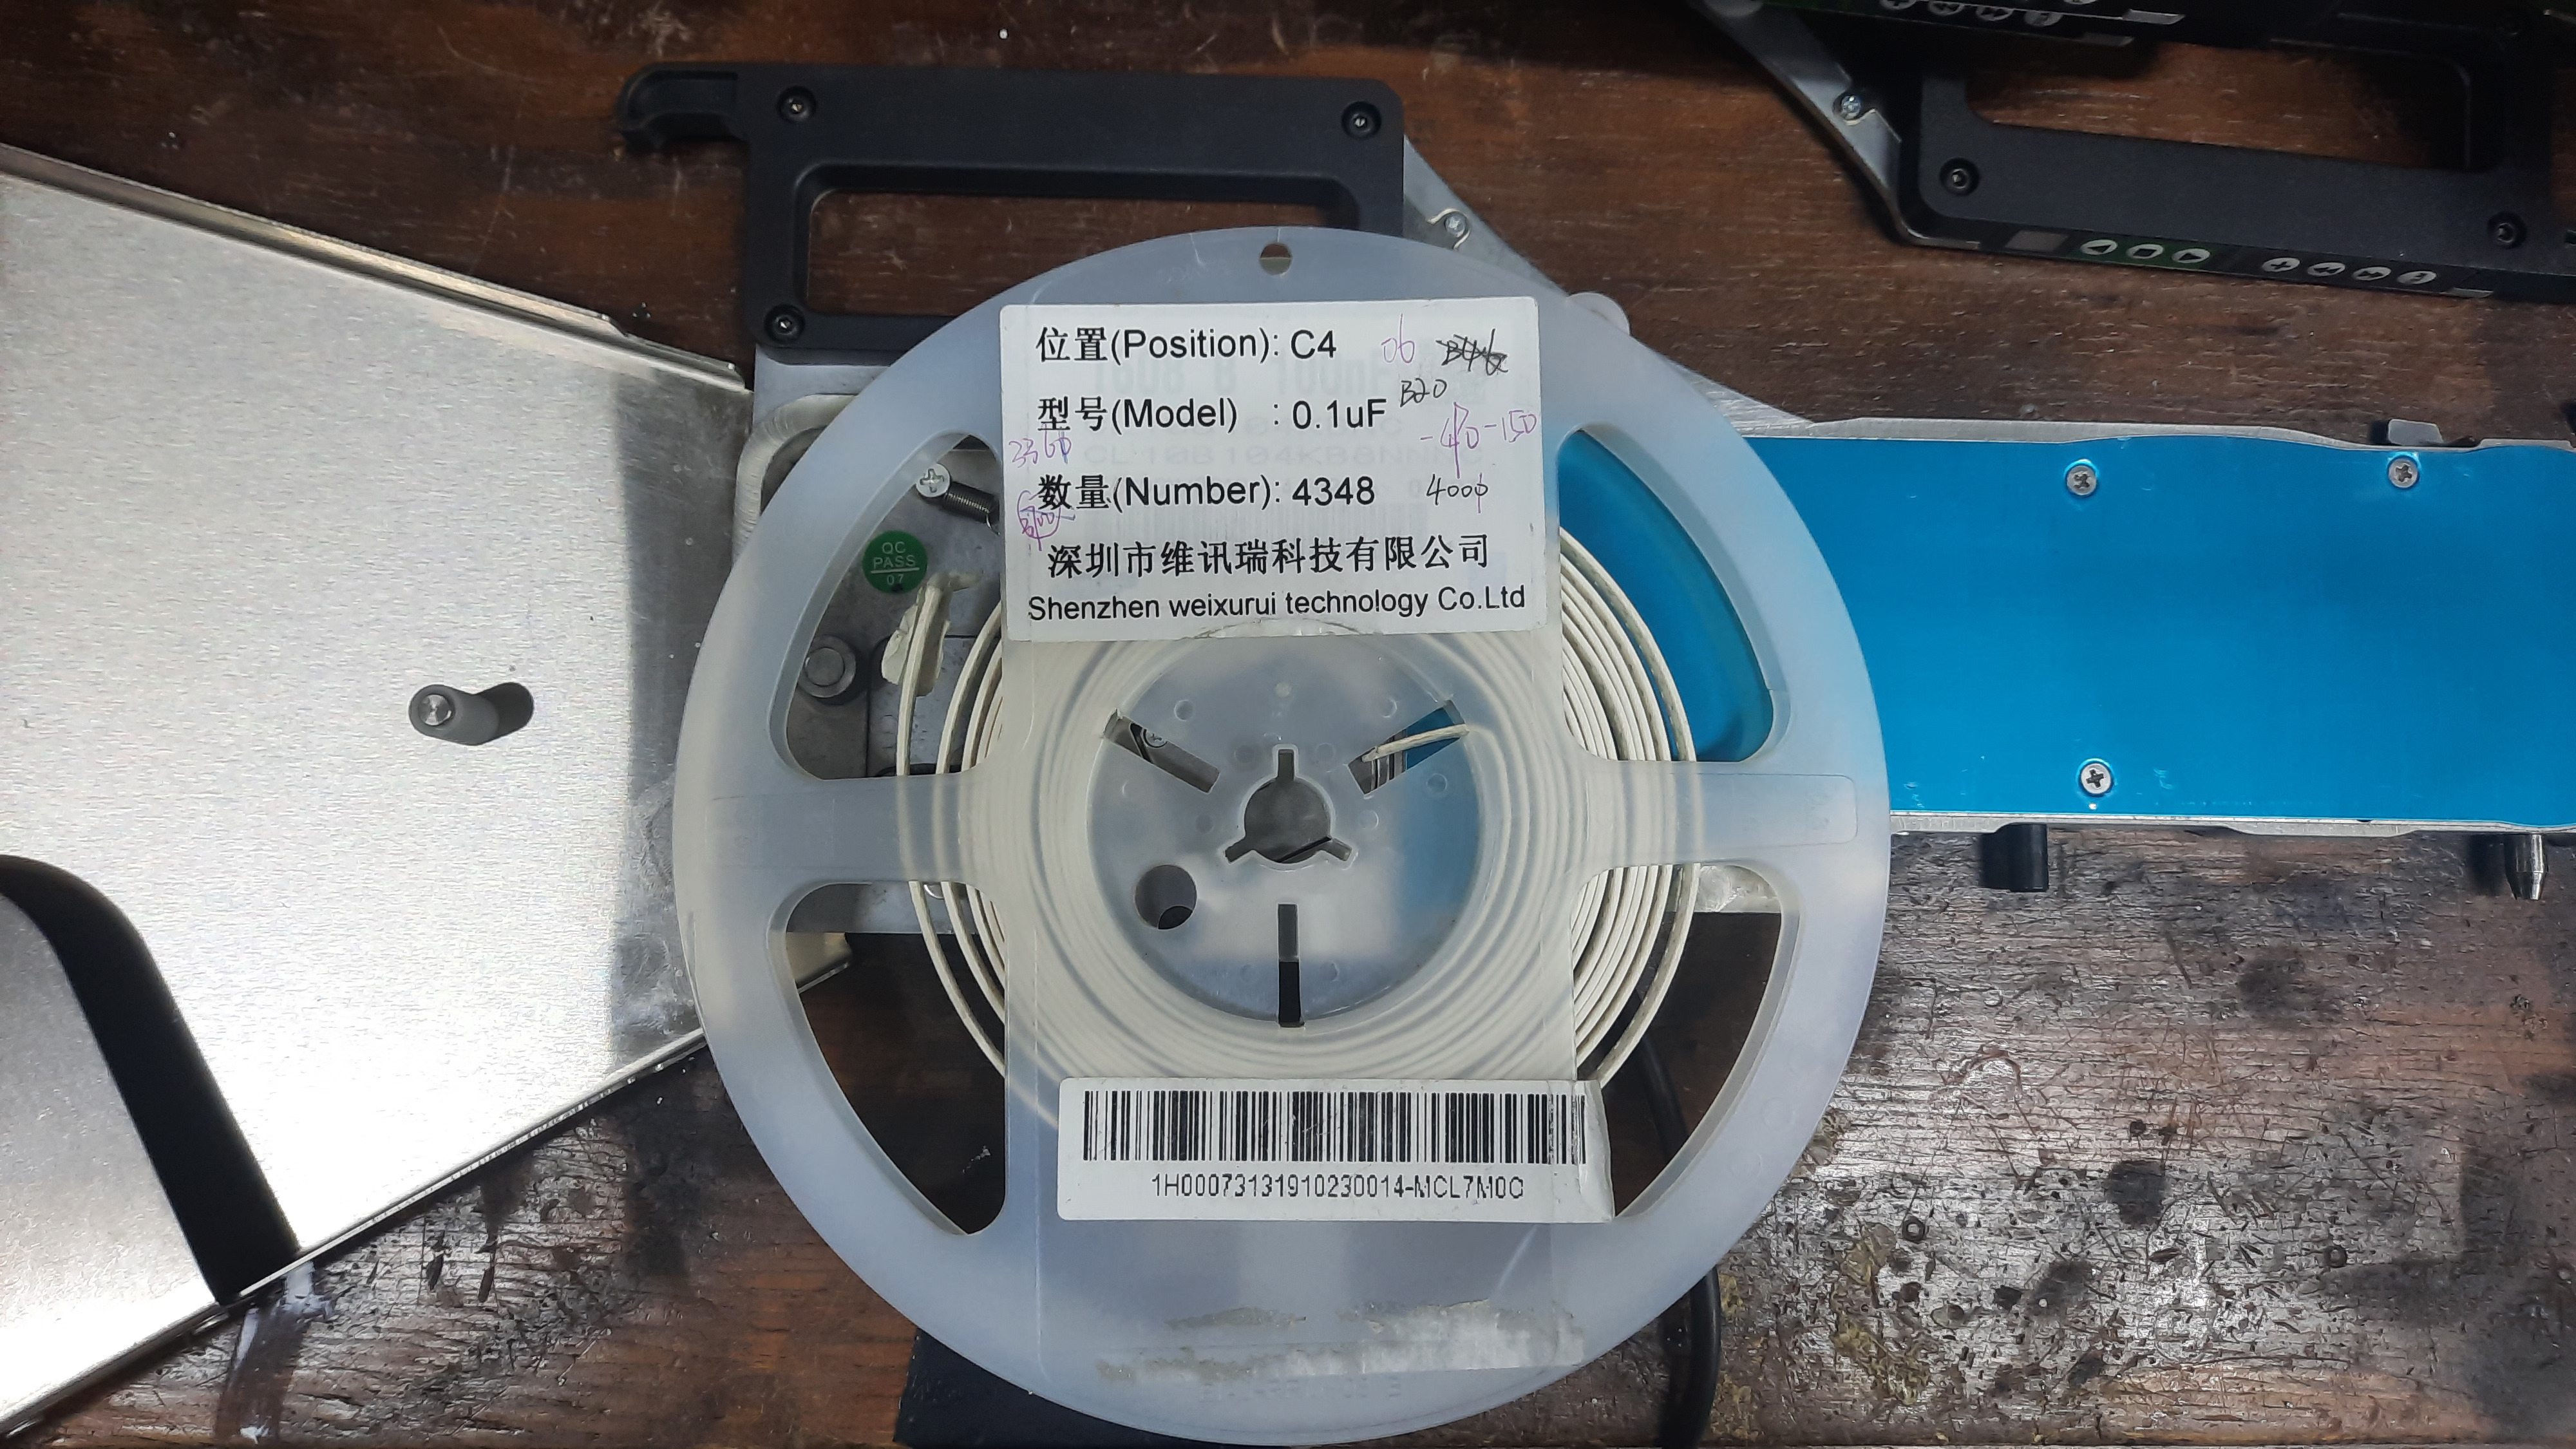
\includegraphics[width=0.9\textwidth]{images/step1.jpg}
 \caption{8mm capacitor tape}
\end{figure}
\newpage
\subsubsection{Step 2: Peeling the cover tape}
Start by peeling around 37cm of the cover tape (The translucent film covering the carrier tape). This will serve to help the feeder automatically pull the cover tape back as it advances the \textbf{carrier tape}.
\begin{figure}[!htb]
 \centering
 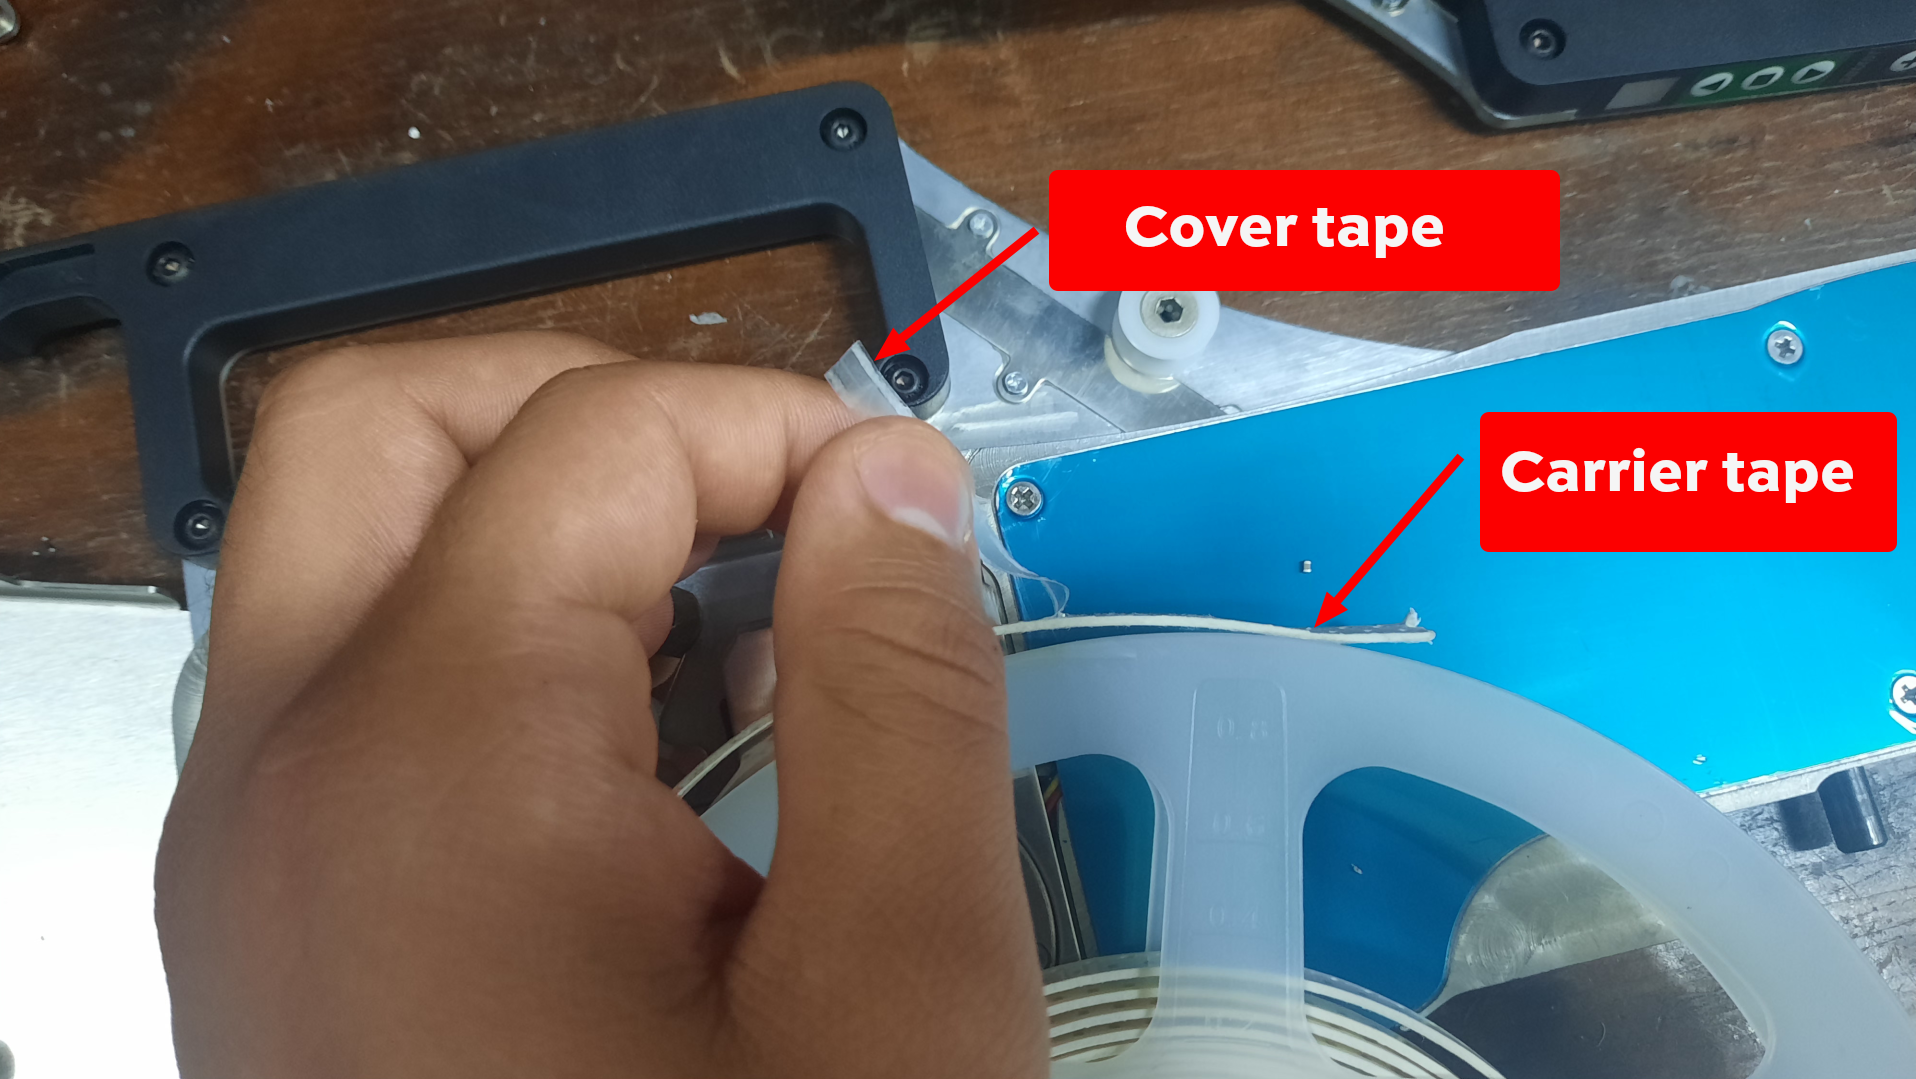
\includegraphics[width=0.9\textwidth]{images/step2.png}
 \caption{Peeling the cover tape}
\end{figure}
\subsubsection{Step 3: Installing the reel in the feeder's base}
Install the reel in the feeder's base, it should be supported by a roll axis which helps it smoothly roll when the tape advances forward.
\begin{figure}[!htb]
 \centering
 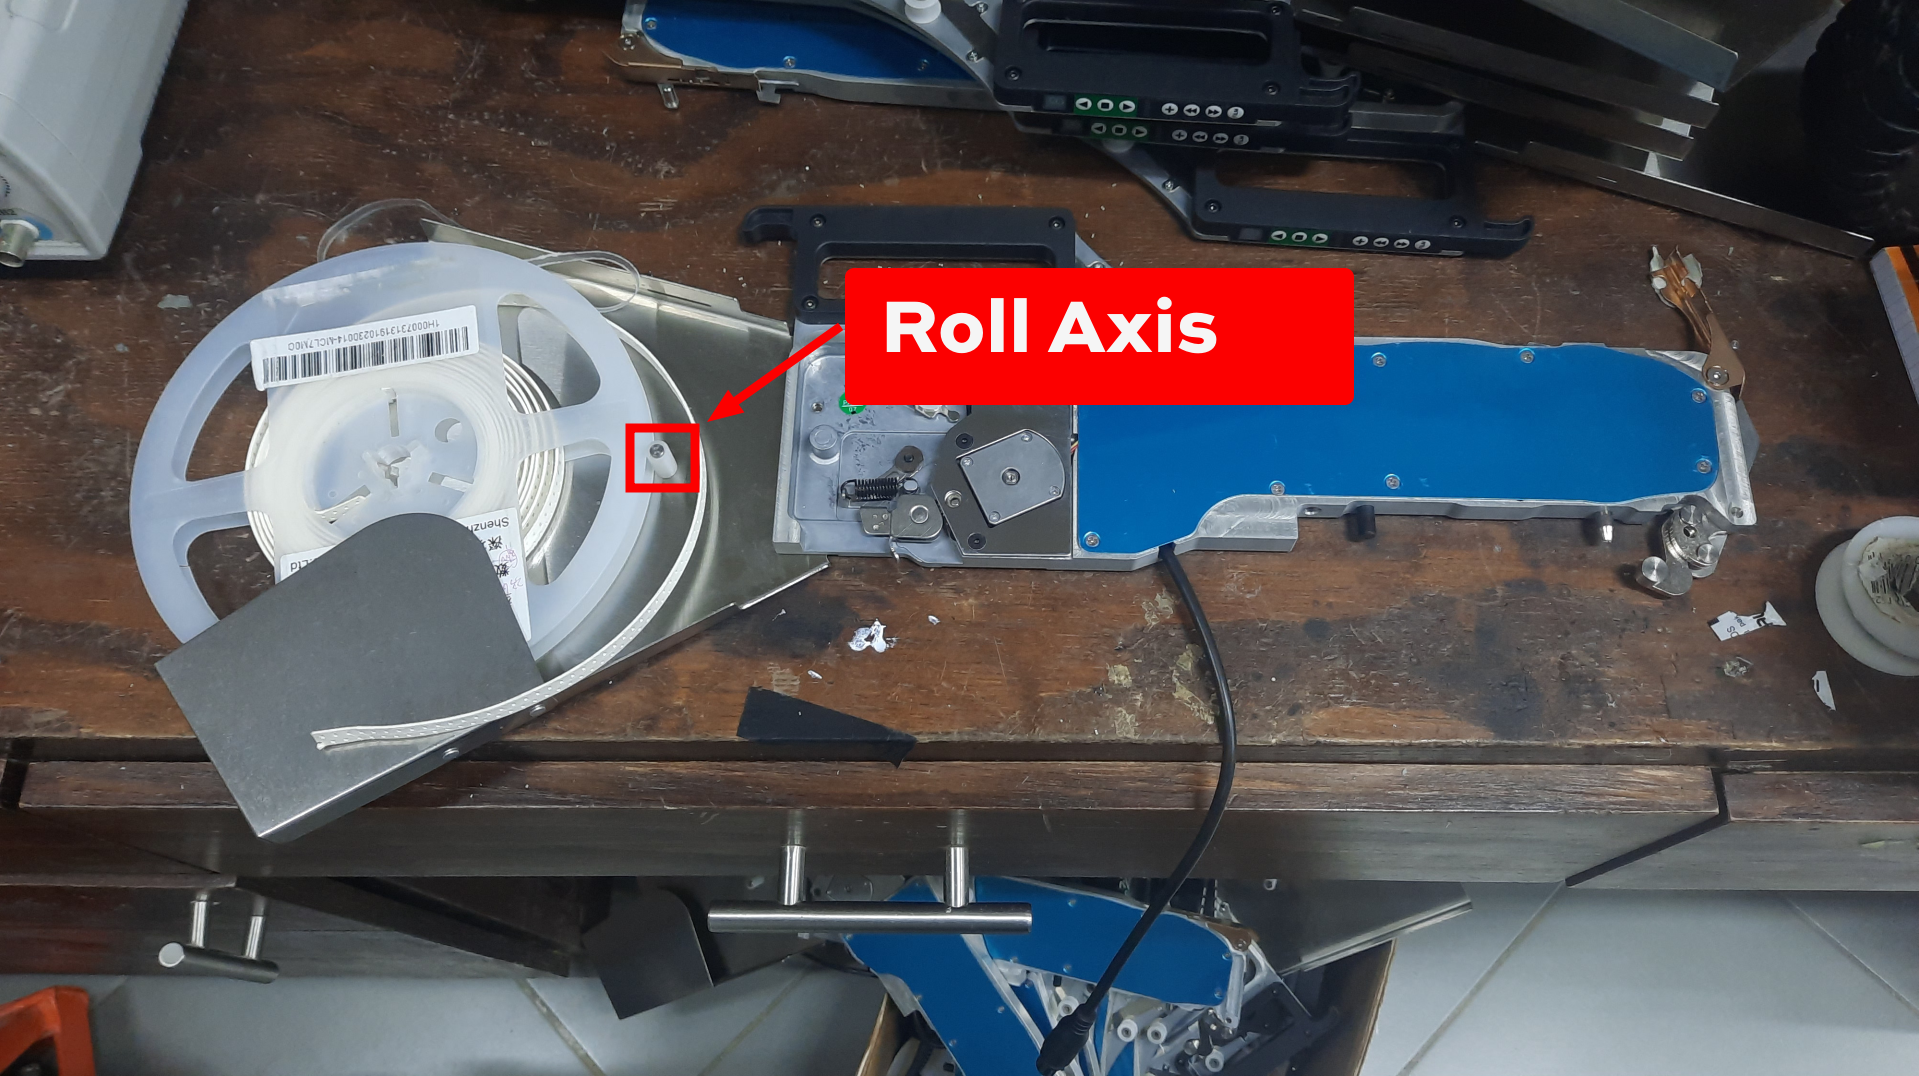
\includegraphics[width=0.9\textwidth]{images/step3.png}
 \caption{Installing the reel in the feeder's base}
\end{figure}
\newpage
\subsubsection{Step 4: Open the front latch}
\begin{figure}[!htb]
 \centering
 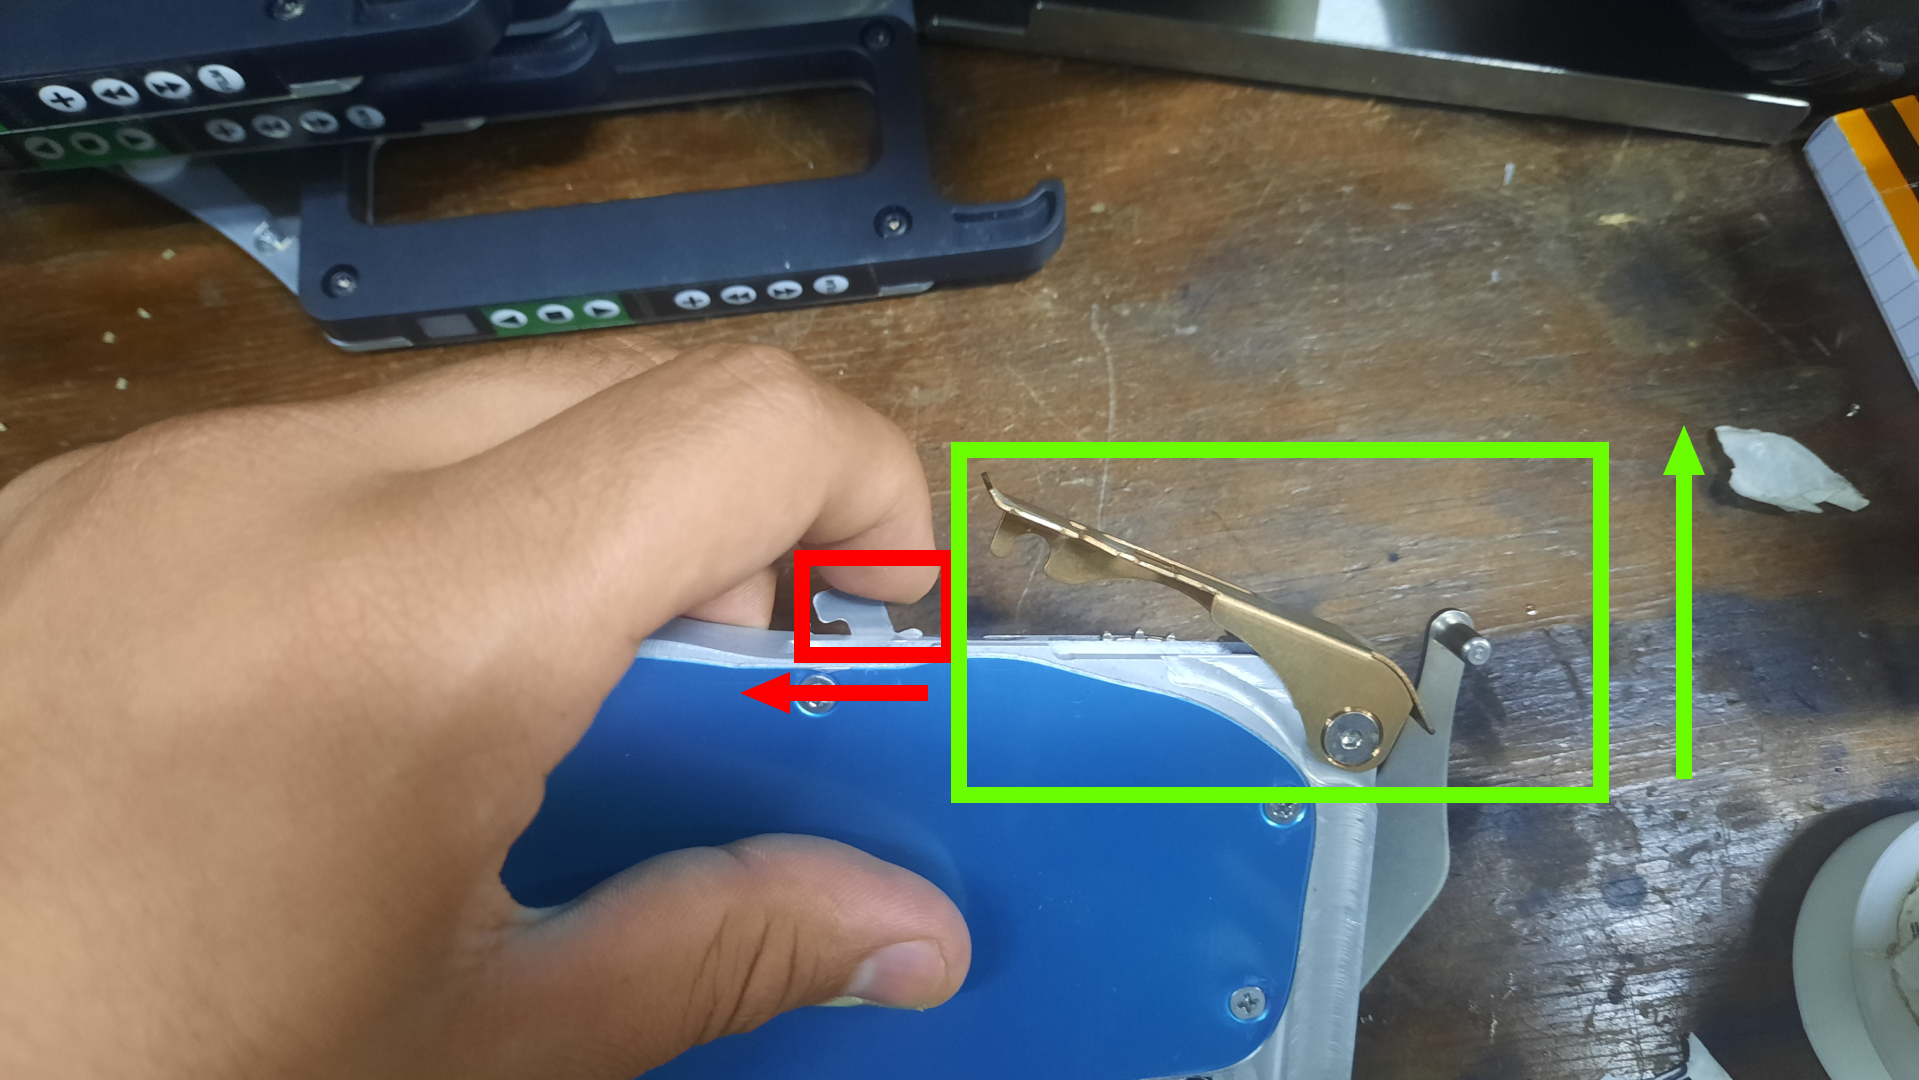
\includegraphics[width=0.9\textwidth]{images/step4.png}
 \caption{Opening the front latch}
\end{figure}
\subsubsection{Step 5: Pass the carrier tape through the latch}
\begin{figure}[!htb]
 \centering
 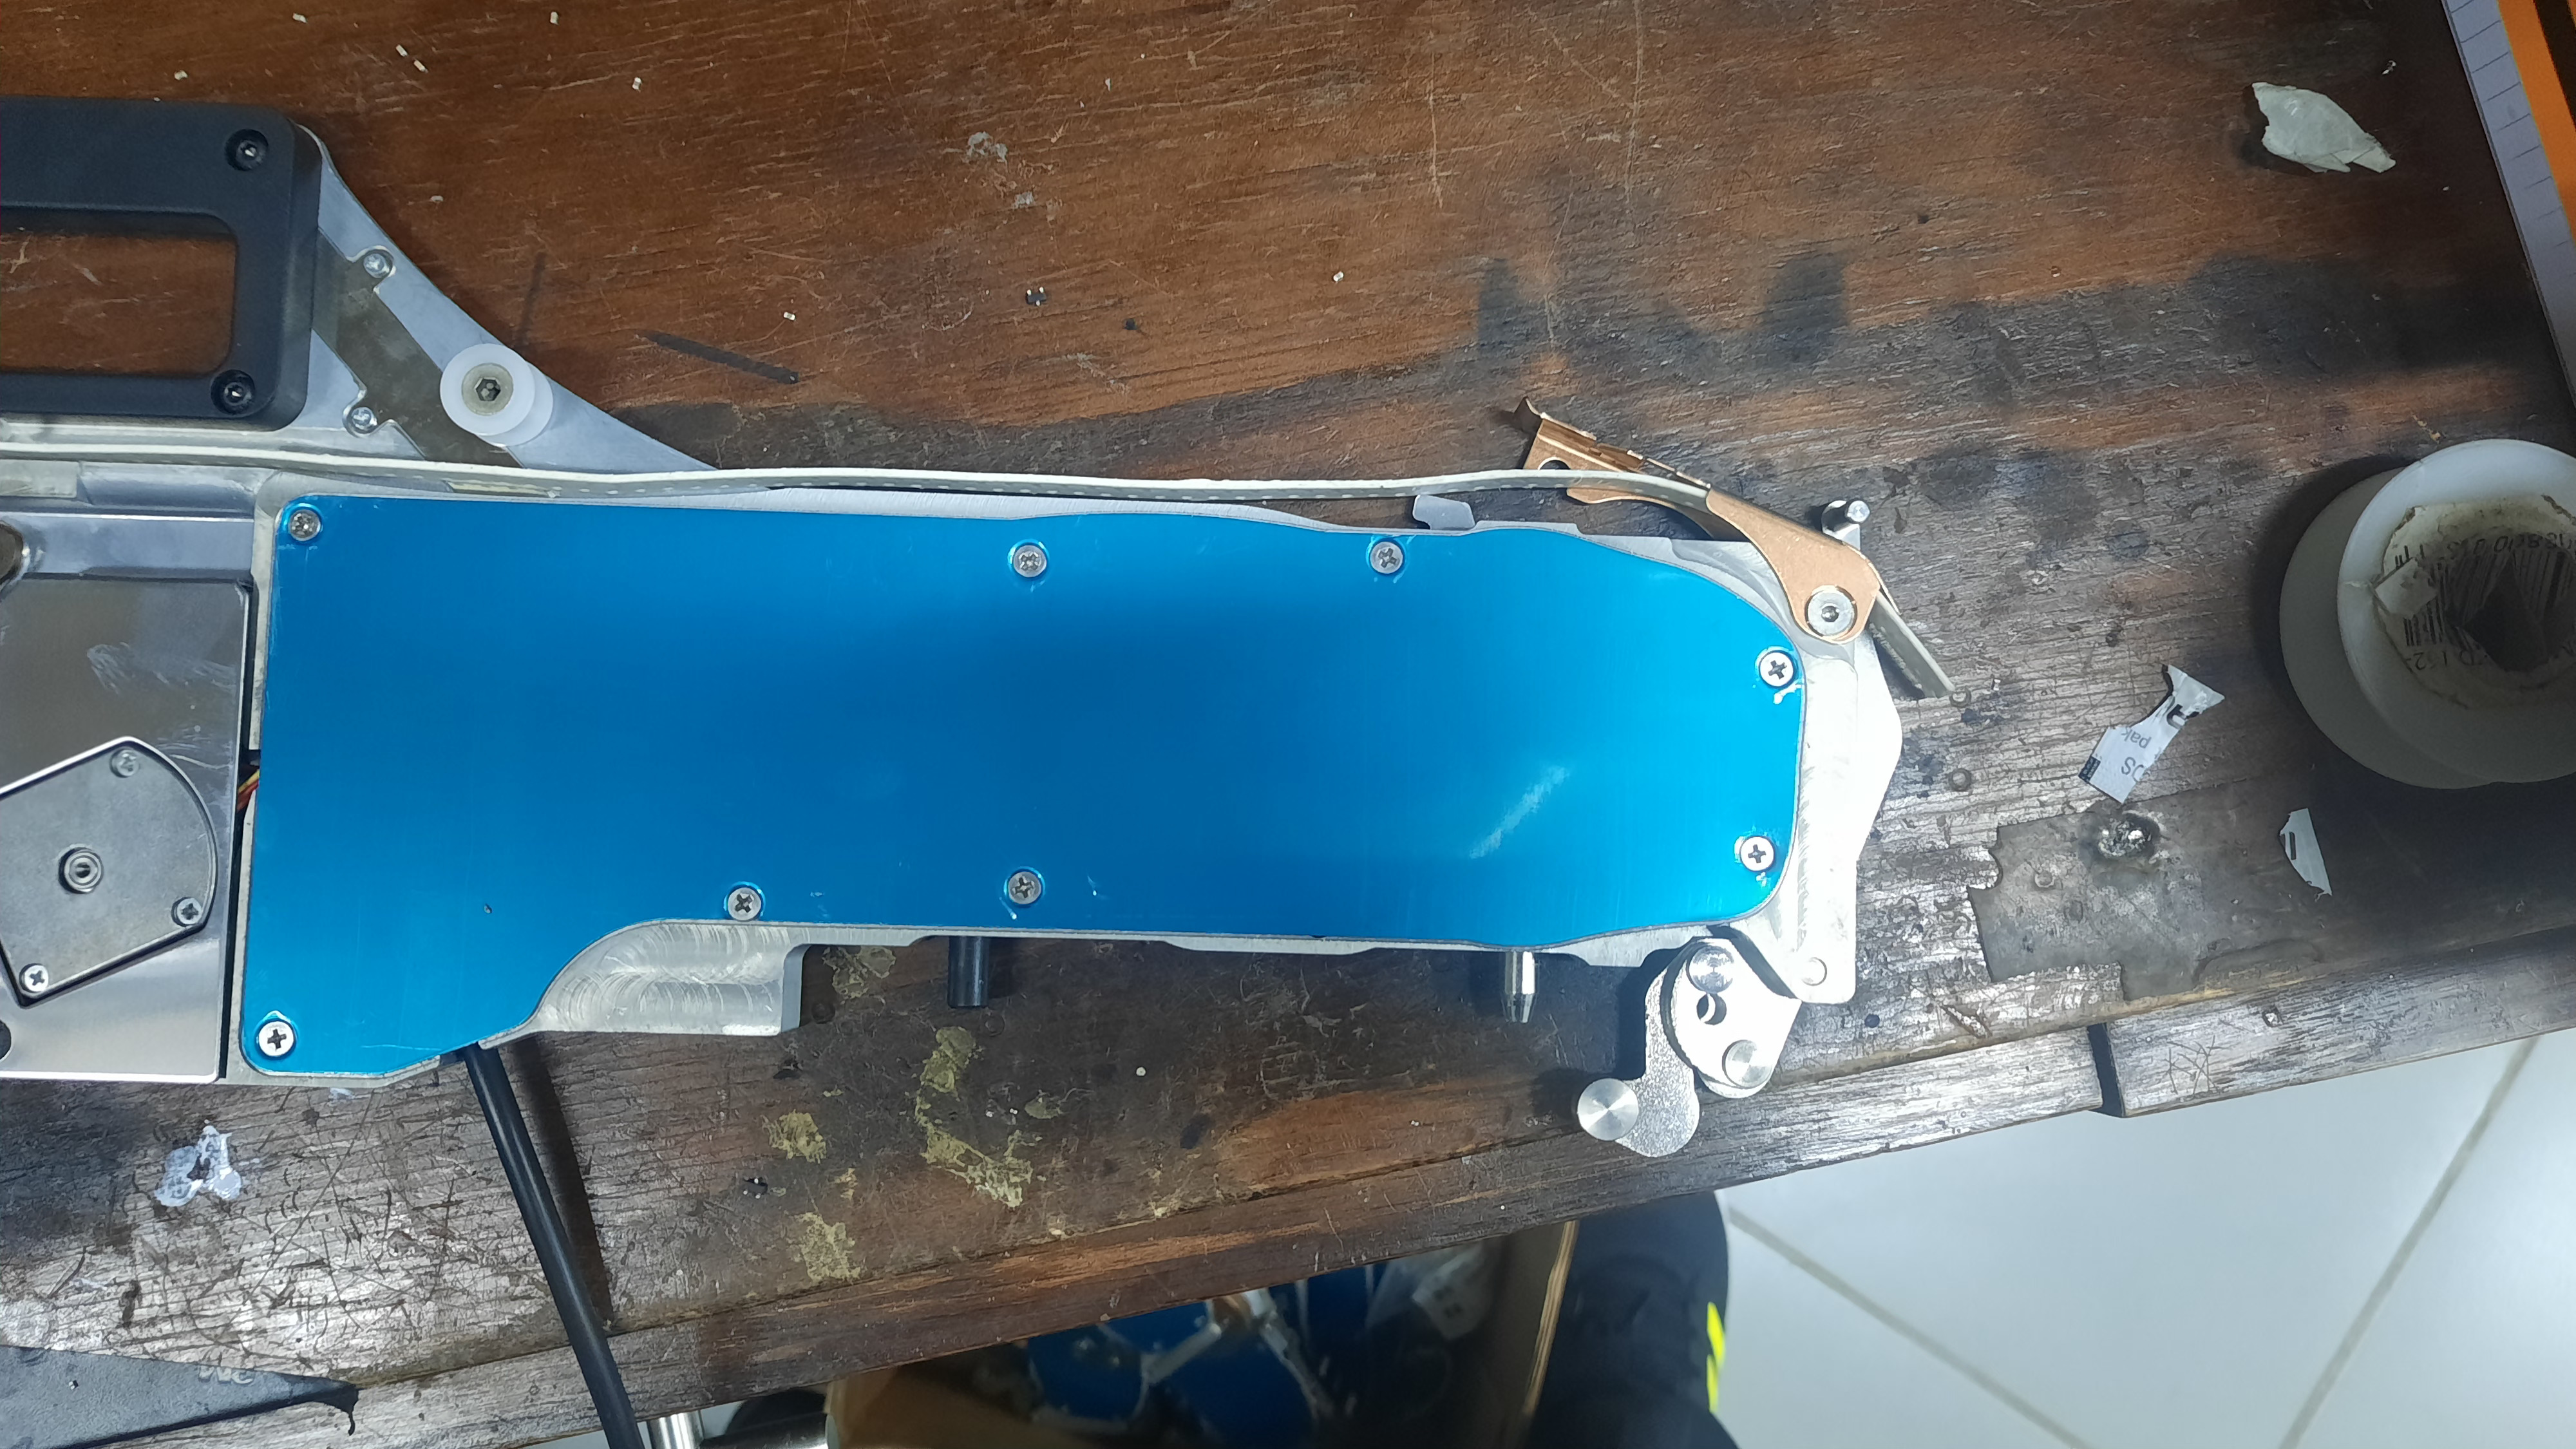
\includegraphics[width=0.9\textwidth]{images/step5.jpg}
 \caption{Passing the carrier tape through the latch}
\end{figure}
\newpage
\subsubsection{Step 6: Close the front latch}
\textbf{Note: } It is important to pass the cover tape by the opening shown in the photo
\begin{figure}[!htb]
 \centering
 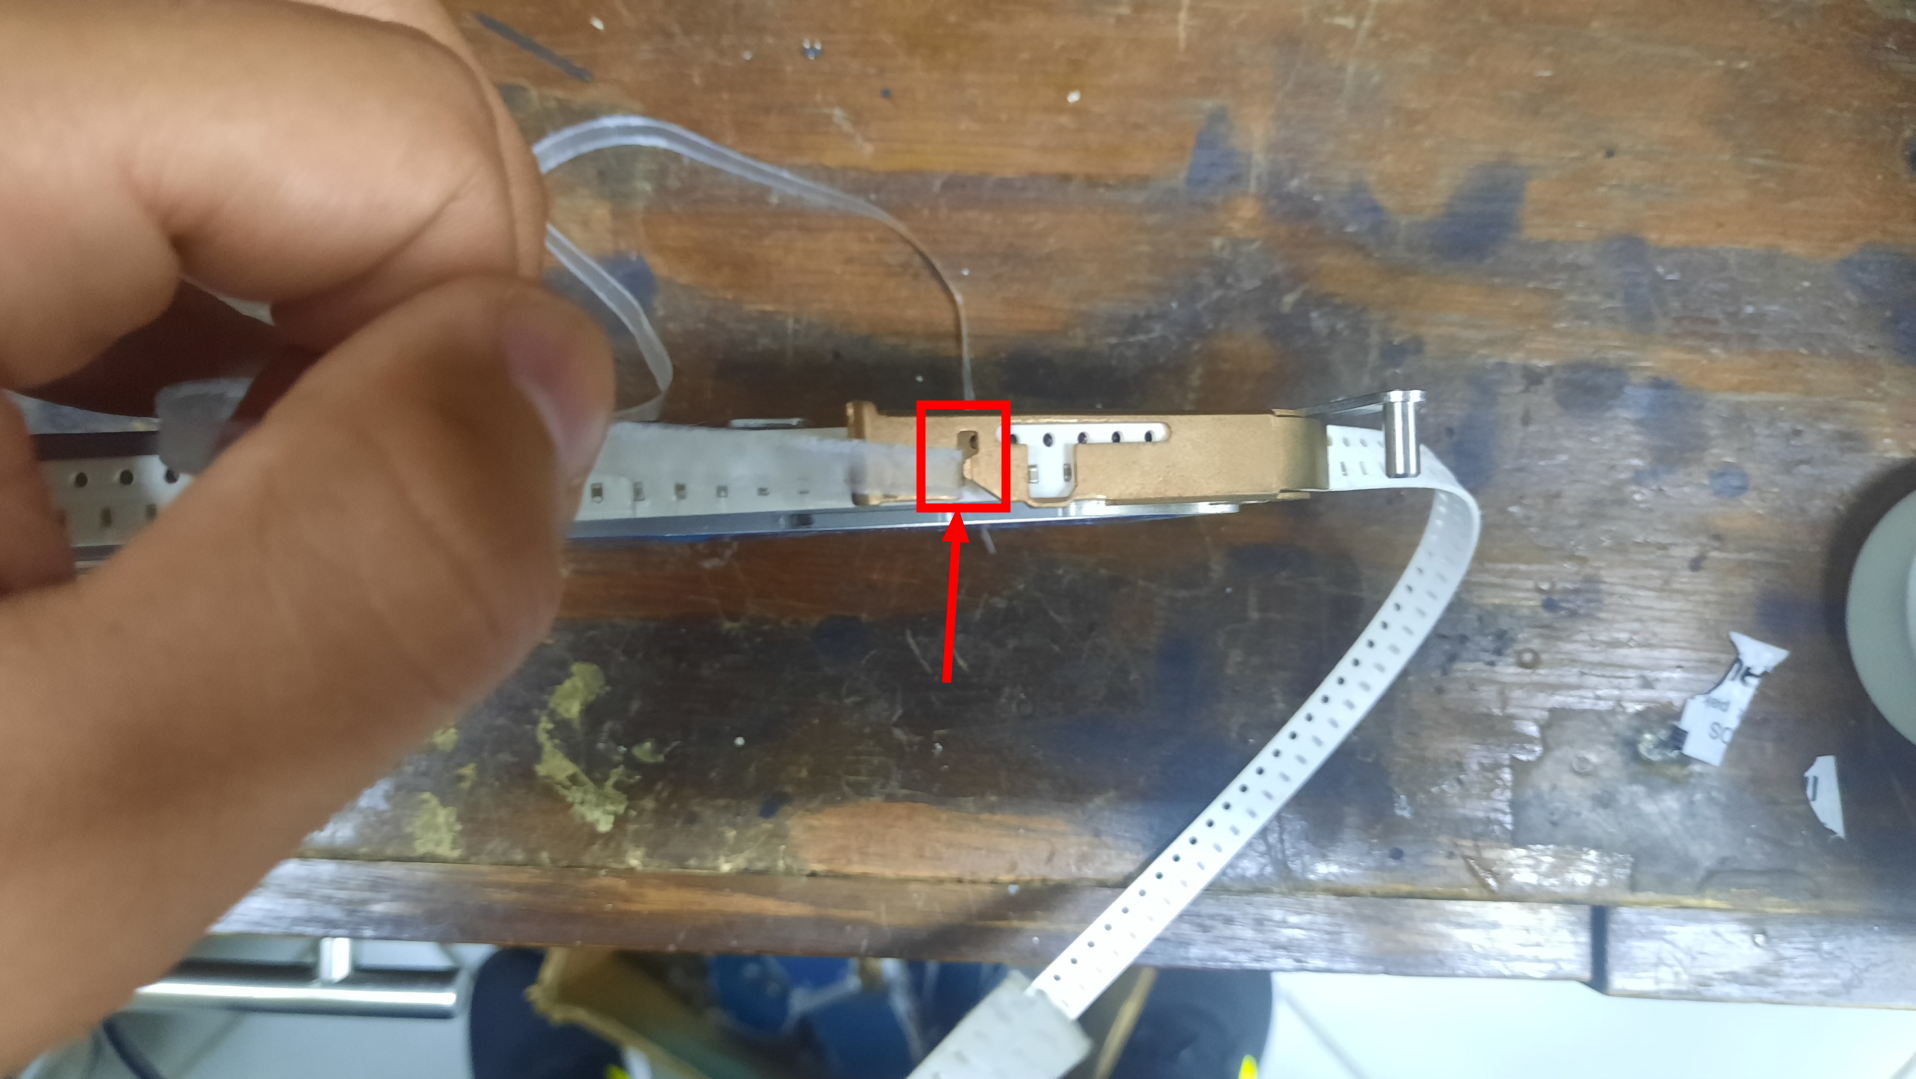
\includegraphics[width=0.9\textwidth]{images/step6.png}
 \caption{Closing the front latch}
\end{figure}
\newpage
\subsubsection{Step 7: Loop back the cover tape}
The cover tape must be looped back to the cover tape peeling mechanism (the tape must be enclosed between the two gears).
\begin{figure}[!htb]
 \centering
 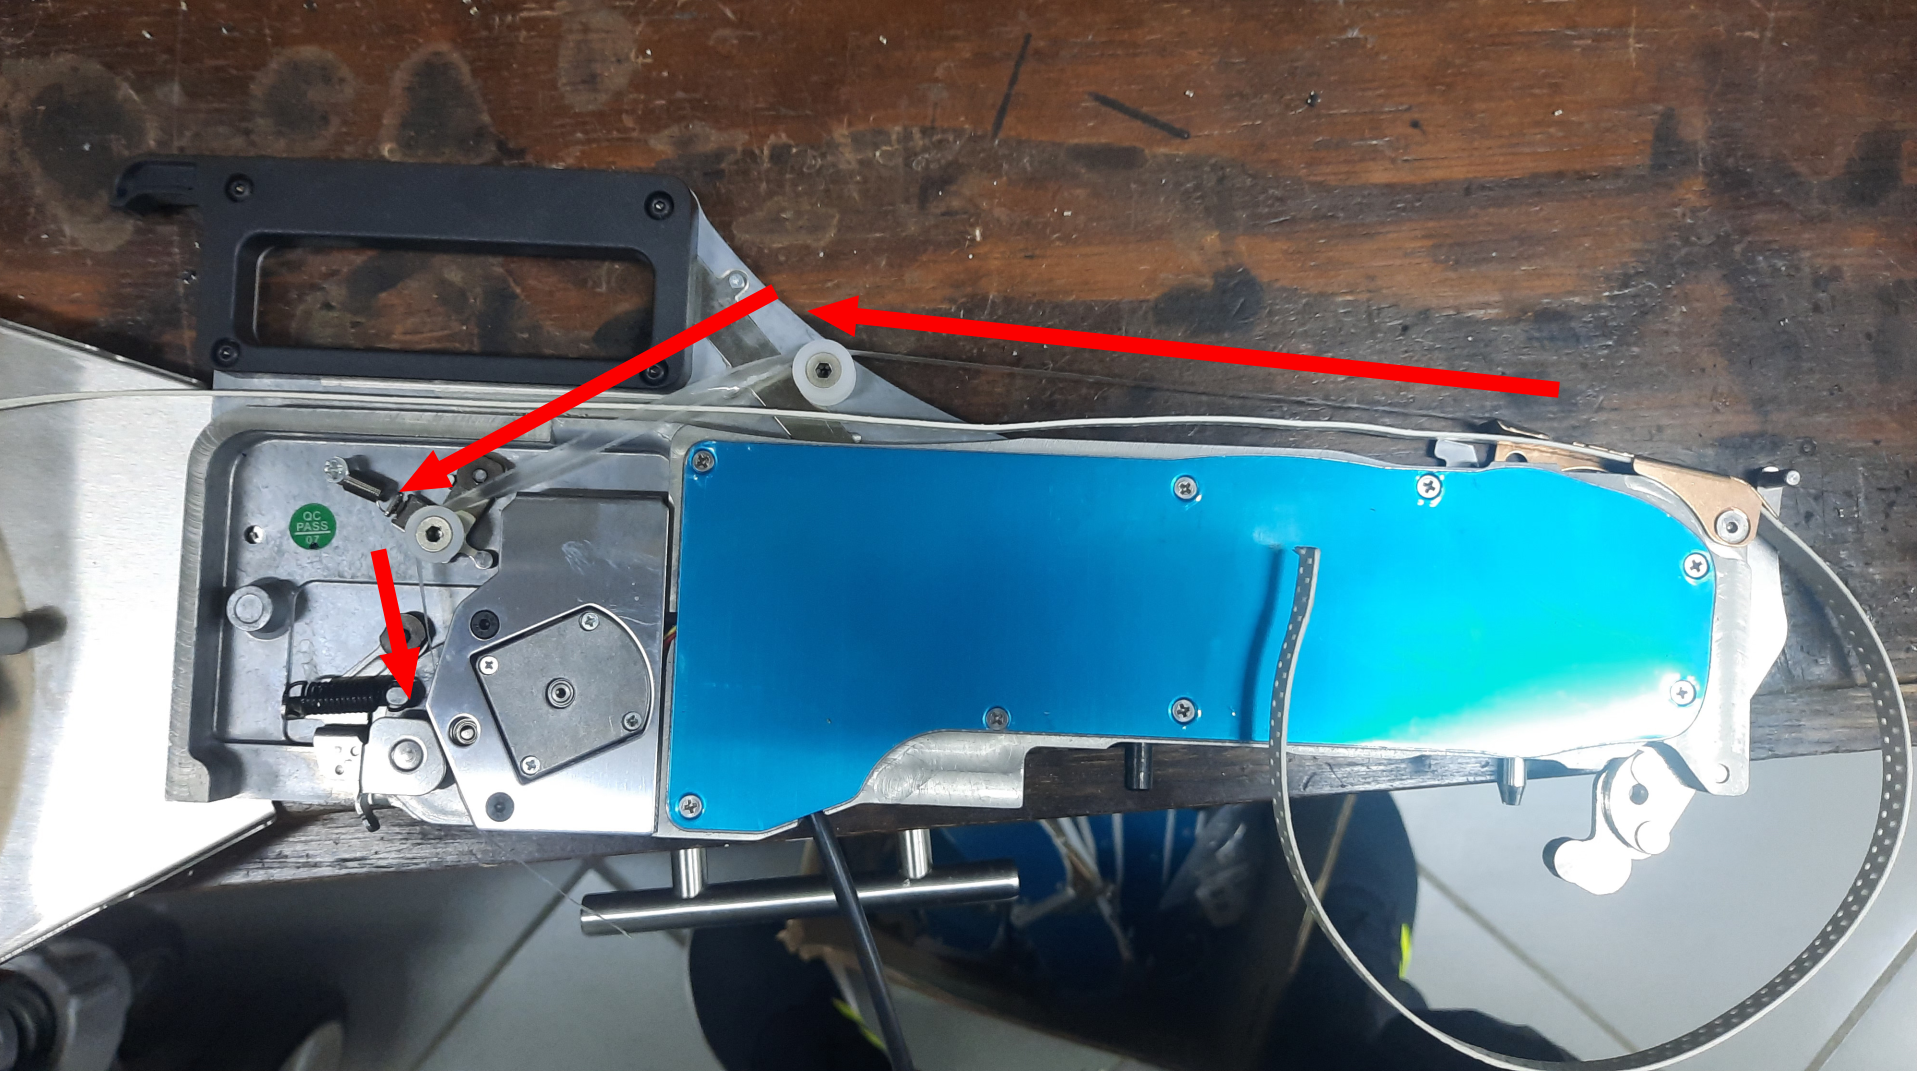
\includegraphics[width=1\textwidth]{images/step7.png}
 \caption{Cover tape loopback trajectory}
\end{figure}
\begin{figure}[!htb]
 \centering
 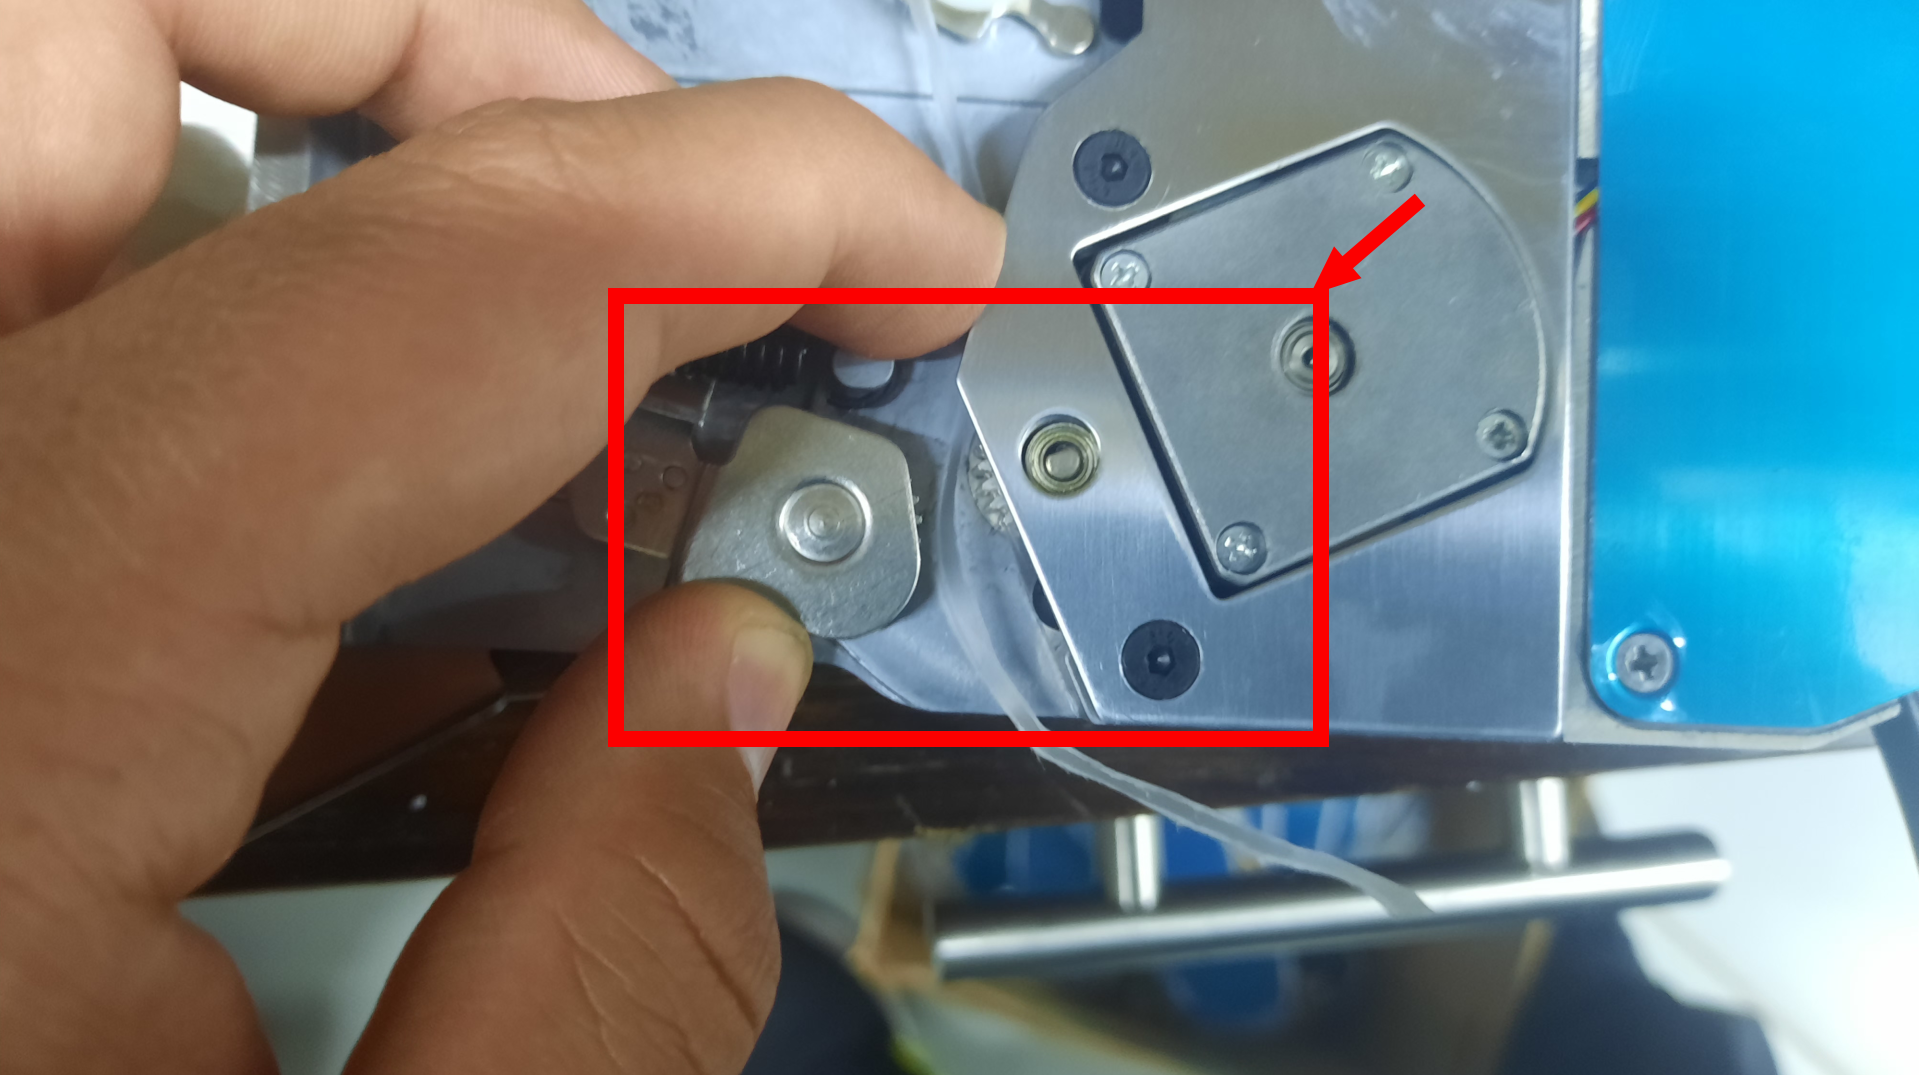
\includegraphics[width=1\textwidth]{images/peeler.png}
 \caption{Cover tape peeling mechanism}
\end{figure}
\newpage
\subsubsection{Step 8: Mount the feeder}
Place the two alignment pins in the corresponding holes on the pick and place machine to mount it in the chosen slot.
\begin{figure}[!htb]
 \centering
 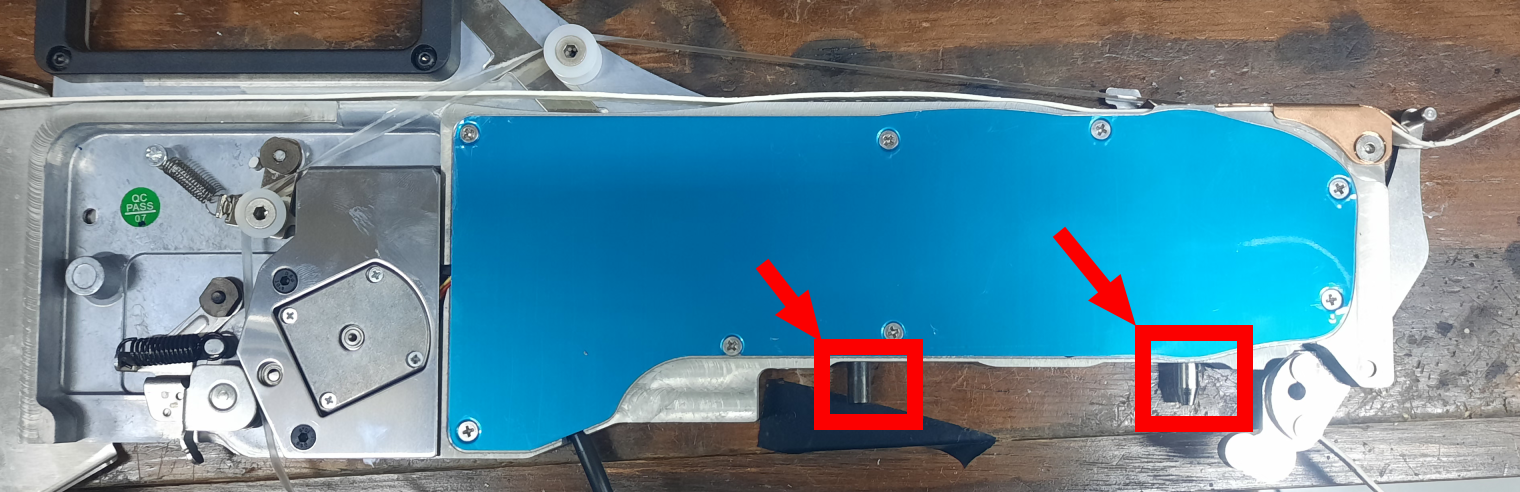
\includegraphics[width=1\textwidth]{images/alignment_pins.png}
 \caption{The feeders' alignment pins}
\end{figure}
\begin{figure}[!htb]
 \centering
 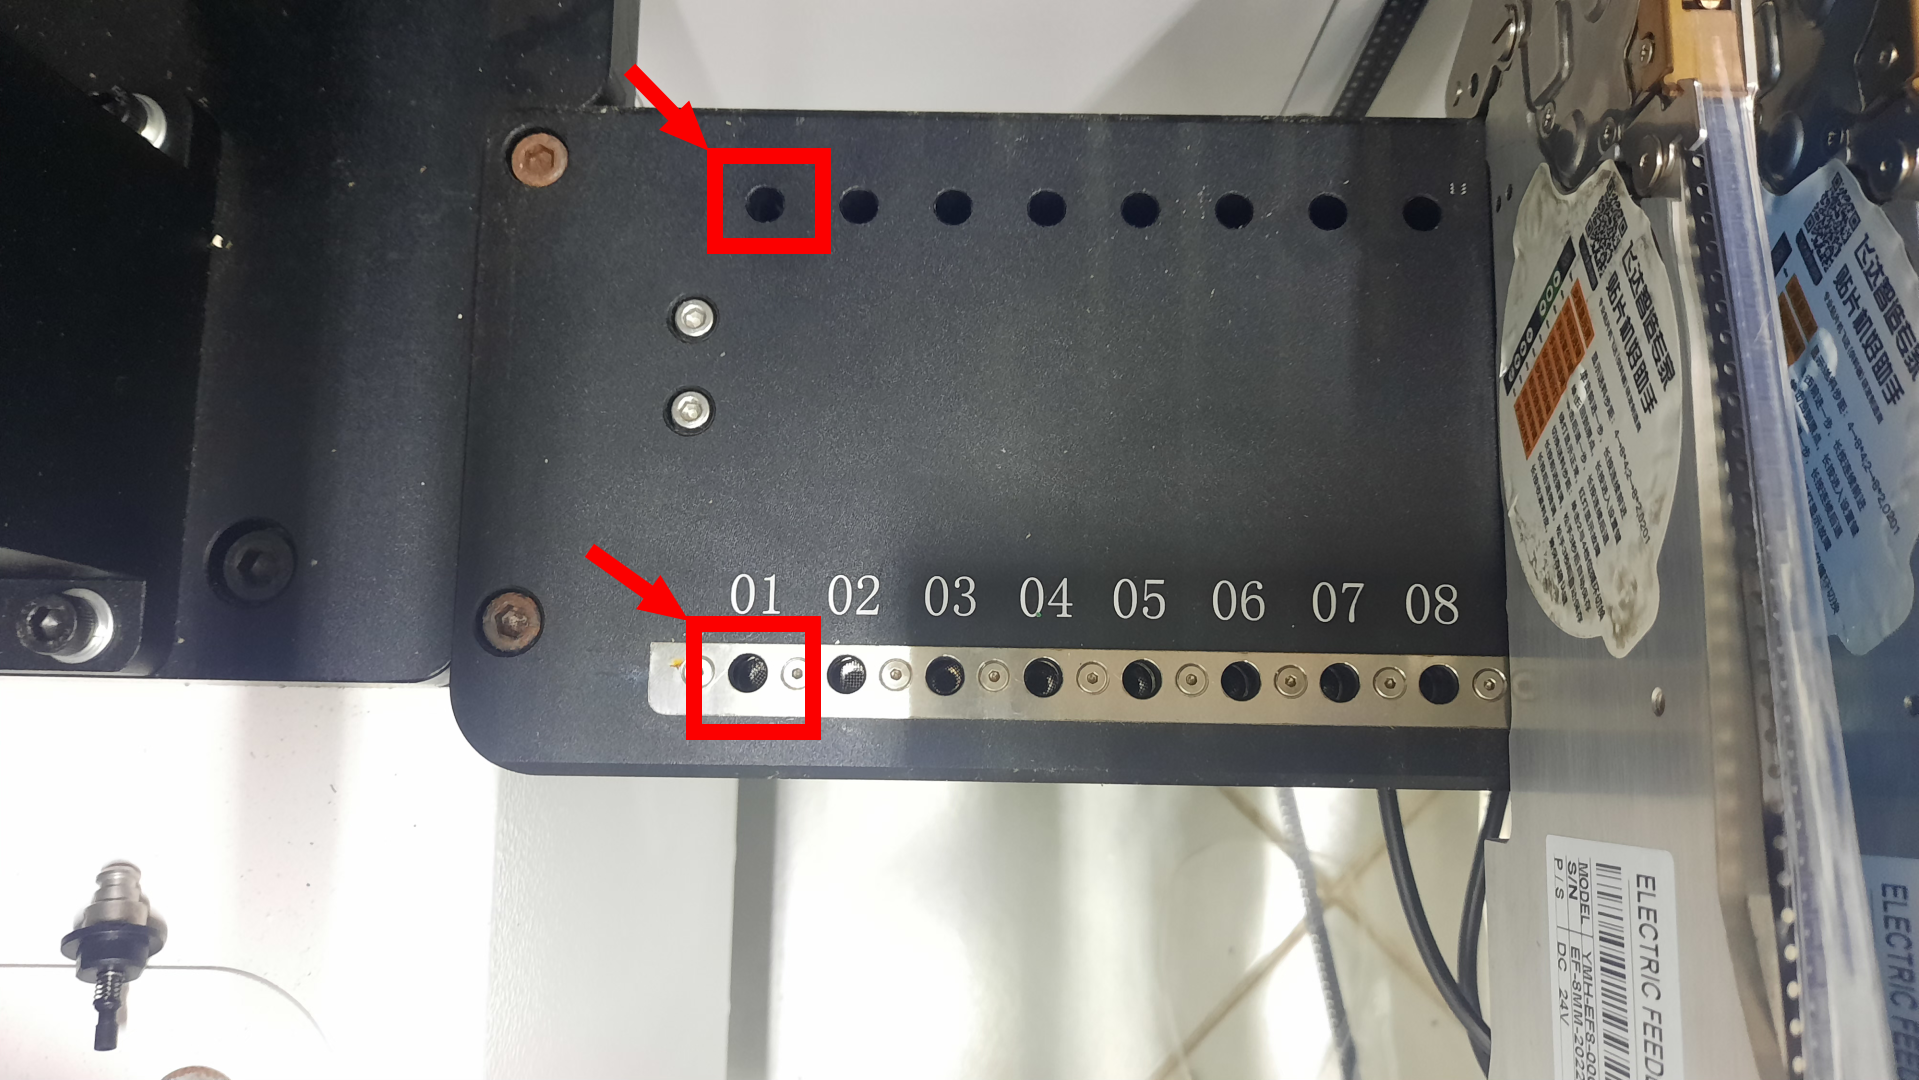
\includegraphics[width=1\textwidth]{images/alignment_holes.png}
 \caption{Feeder slot 1 alignment holes}
\end{figure}
\newpage
\subsubsection{Step 9: Lock in the feeder}
Push the locking latch in the direction indicated by the photo to lock the feeder in.
\begin{figure}[!htb]
 \centering
 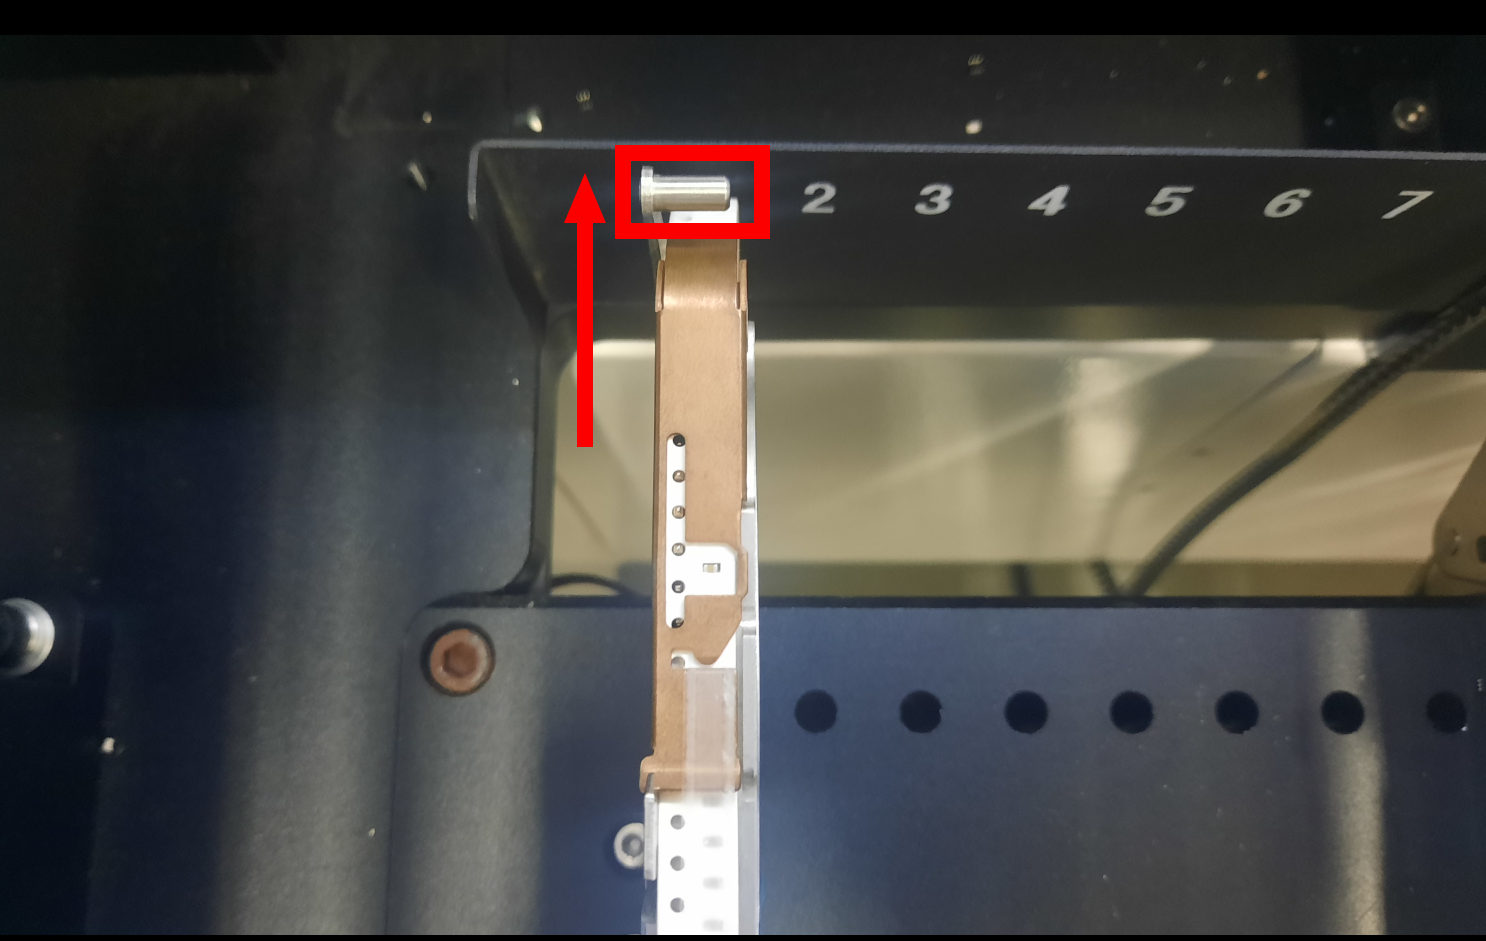
\includegraphics[width=0.9\textwidth]{images/step9.png}
 \caption{Locking in the feeder}
\end{figure}
\subsubsection{Step 10: Plug the feeder in}
\textbf{Note: } It is important to connect the feeder to the plug corresponding to its slot in the pick and place machine. The plugs for even numbered slots are placed high, and odd numbered slot plugs are placed low.
\begin{figure}[!htb]
 \centering
 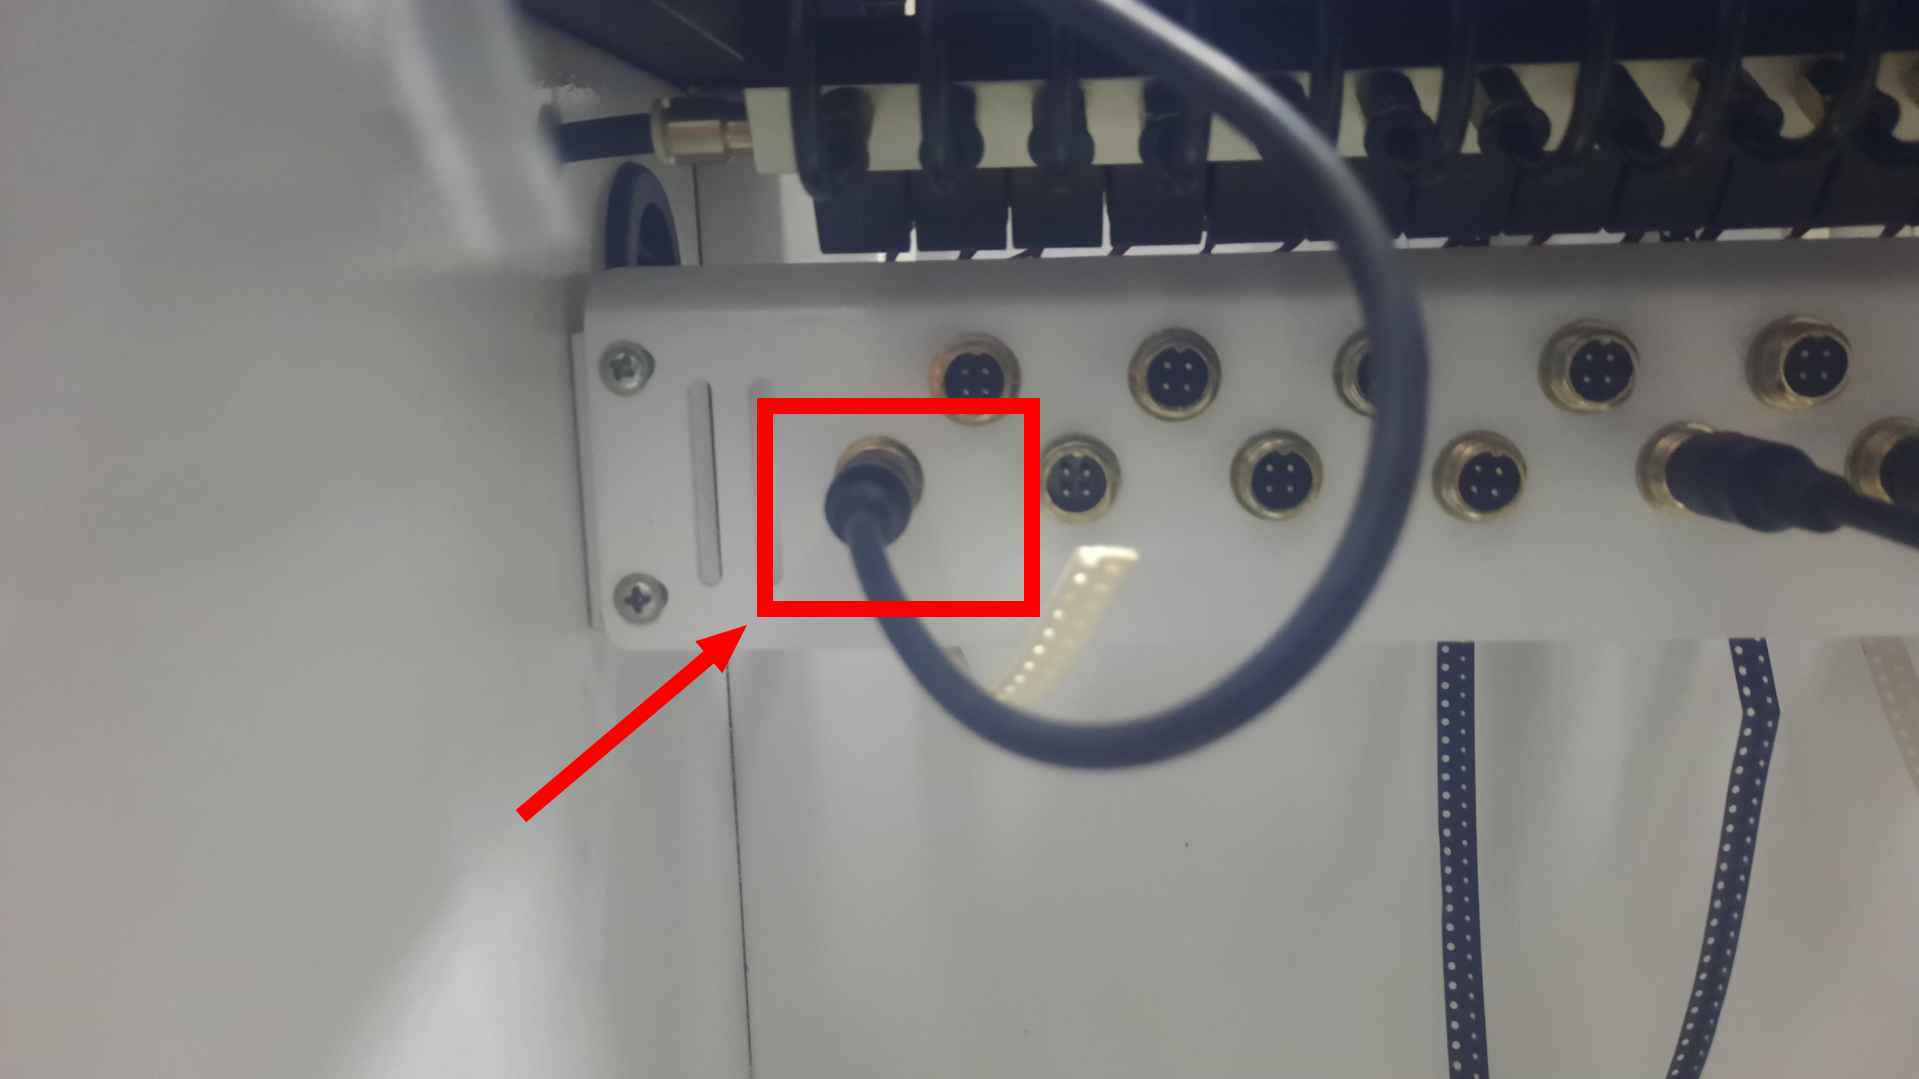
\includegraphics[width=0.9\textwidth]{images/step10.png}
 \caption{Plugging in the feeder in the feeder}
\end{figure}
\newpage
\subsection{Feeder controls}
\begin{figure}[!htb]
 \centering
 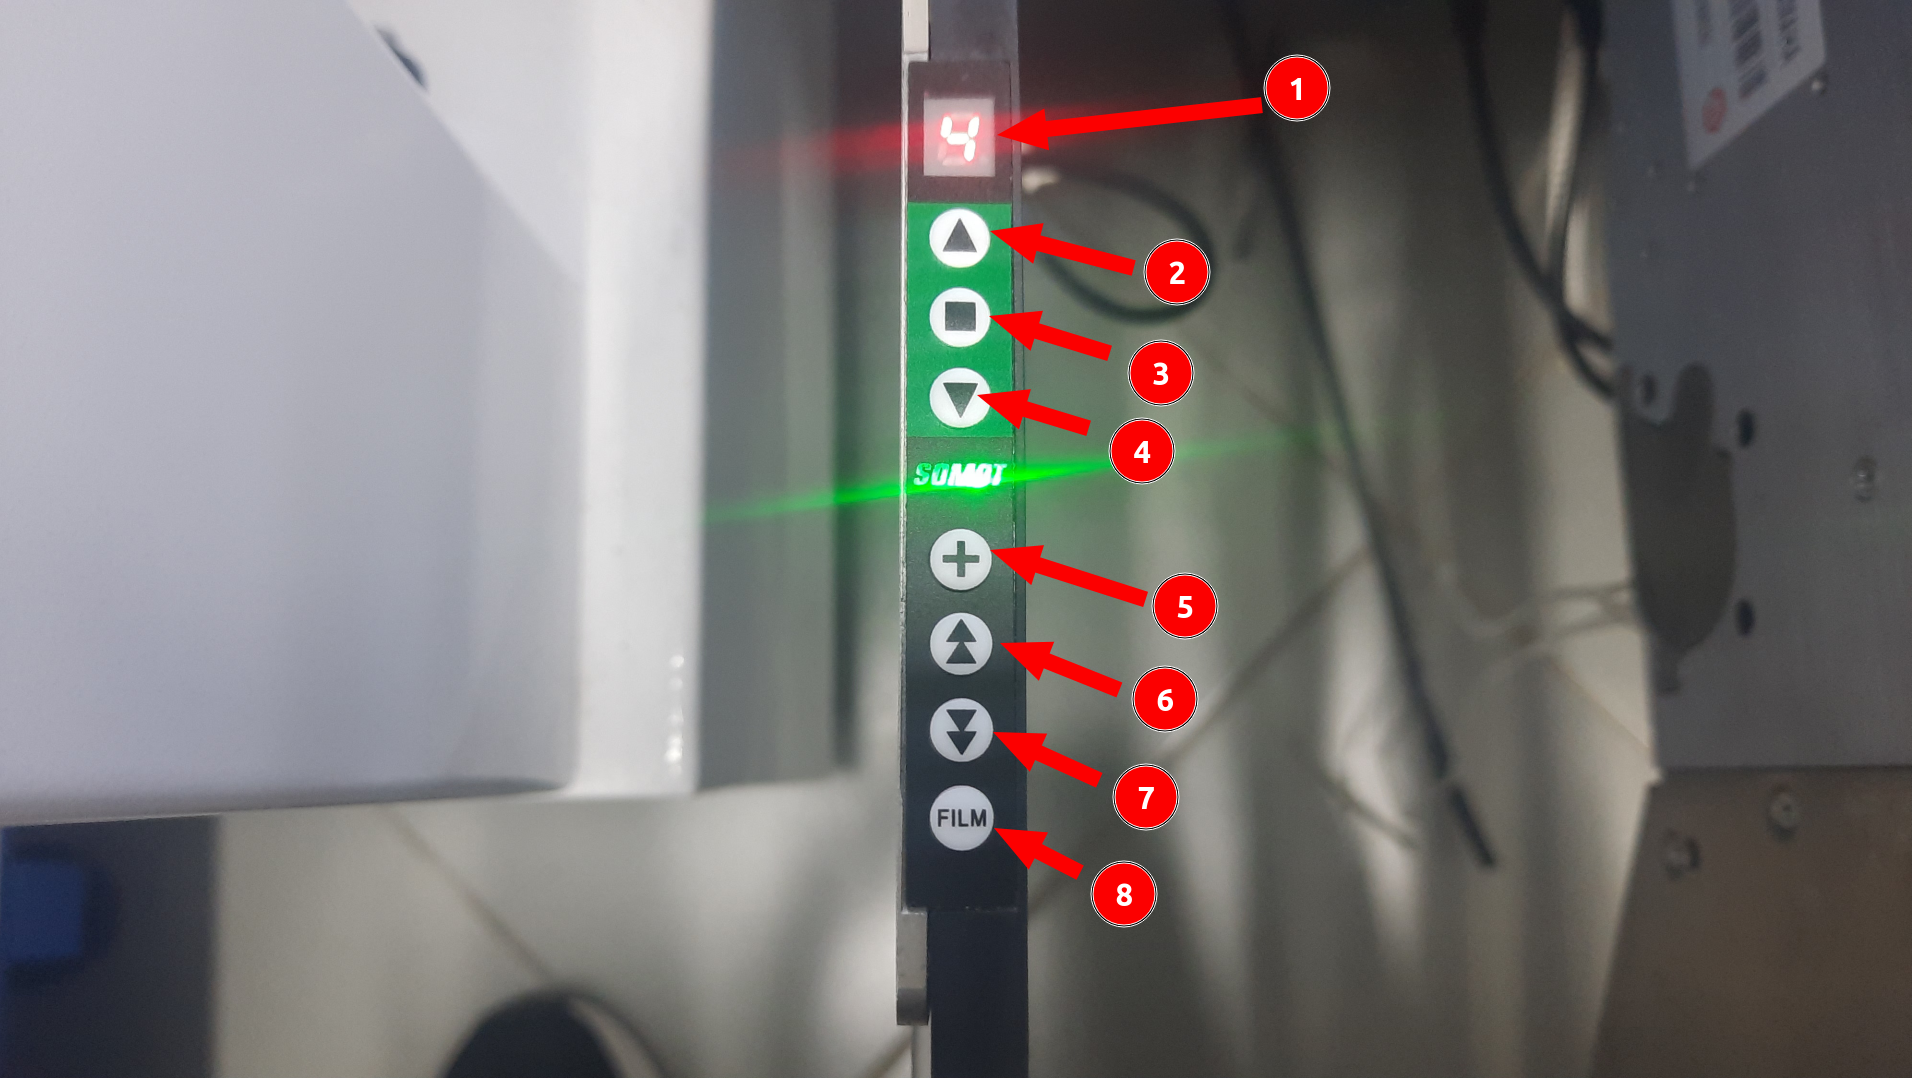
\includegraphics[width=1\textwidth]{images/controls.png}
 \caption{Feeder front controls}
\end{figure}
\begin{itemize}
 \item \textbf{1: } Current step mode (4: full step, 2: half step)
 \item \textbf{2: } Step forward
 \item \textbf{3: } Center carrier tape
 \item \textbf{4: } Step backward
 \item \textbf{5: } Switch step mode
 \item \textbf{6: } Micro step forward (advances tape slowly)
 \item \textbf{7: } Micro step backward
 \item \textbf{8: } Pull cover tape
\end{itemize}
\newpage
\subsection{Feeder optimization}
By clicking on \textbf{"Optimize"} a feeder optimization dialog pops up.\\
The user must fill the \textbf{Provider}, \textbf{Noz} , \textbf{Camera}, \textbf{Visual} and \textbf{Loop Mode}. Let's explain what some of these columns are:
\begin{itemize}
 \item \textbf{Provider: } Meaning the type of feeder that will be providing the component.
 \item \textbf{Noz: } The nozzle size compatible with the component's package.
 \item \textbf{Camera: } The camera responsible for component recognition.
 \item \textbf{Loop Mode: } Refers to the control algorithm used for the pick and place process.
\end{itemize}
\begin{figure}[!htb]
 \centering
 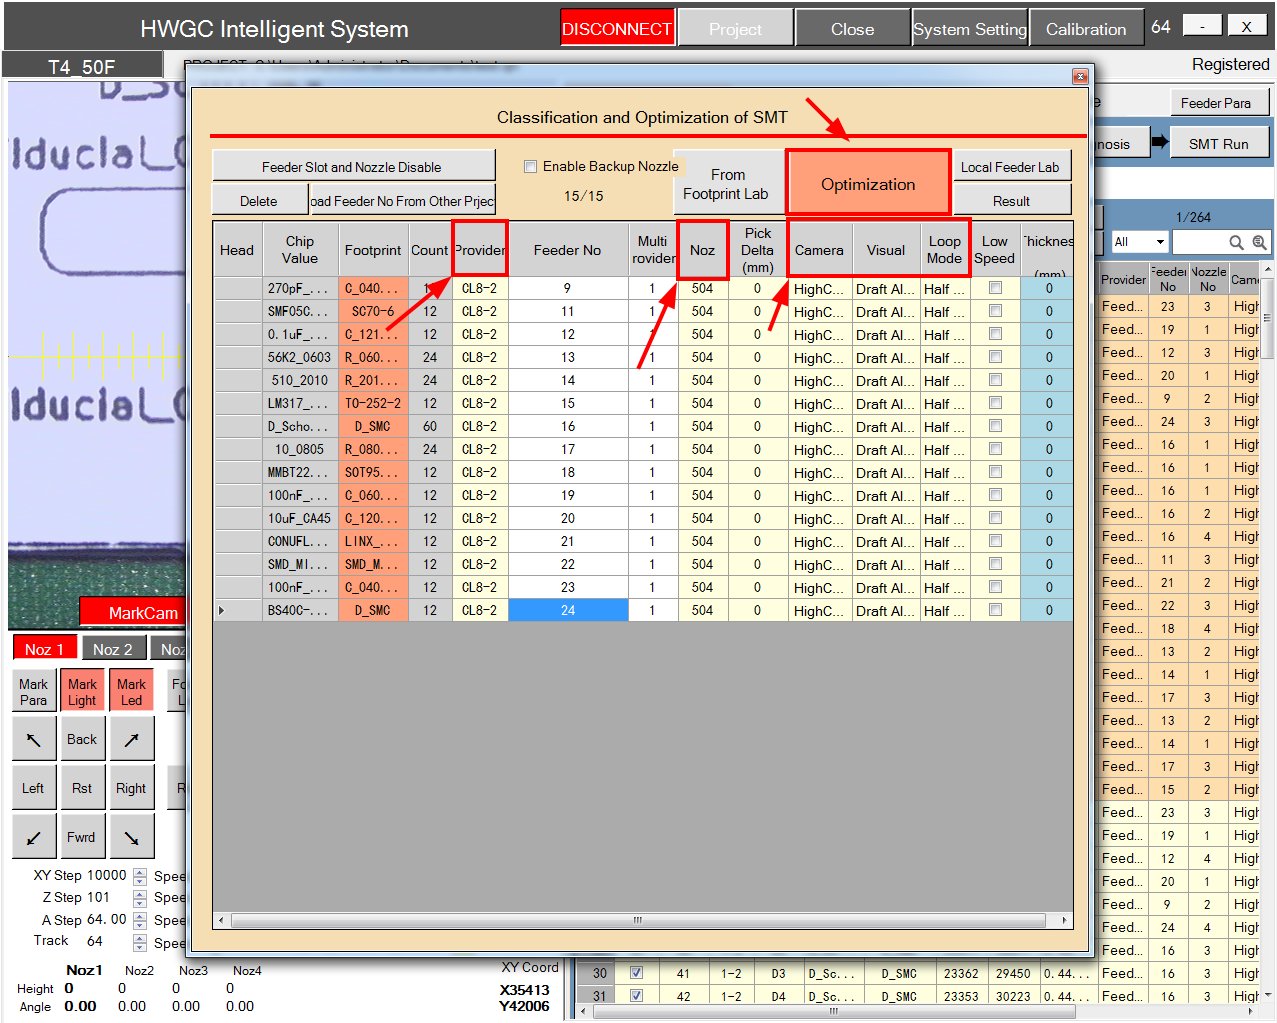
\includegraphics[width=1\textwidth]{images/scrot18.png}
 \caption{Feeder optimization window}
\end{figure}
Clicking on the \textbf{"Optimization"} button will associate each component feeder with an optimal feeder slot, to miminize travel distance and pick time.
\newpage
\begin{figure}[!htb]
 \centering
 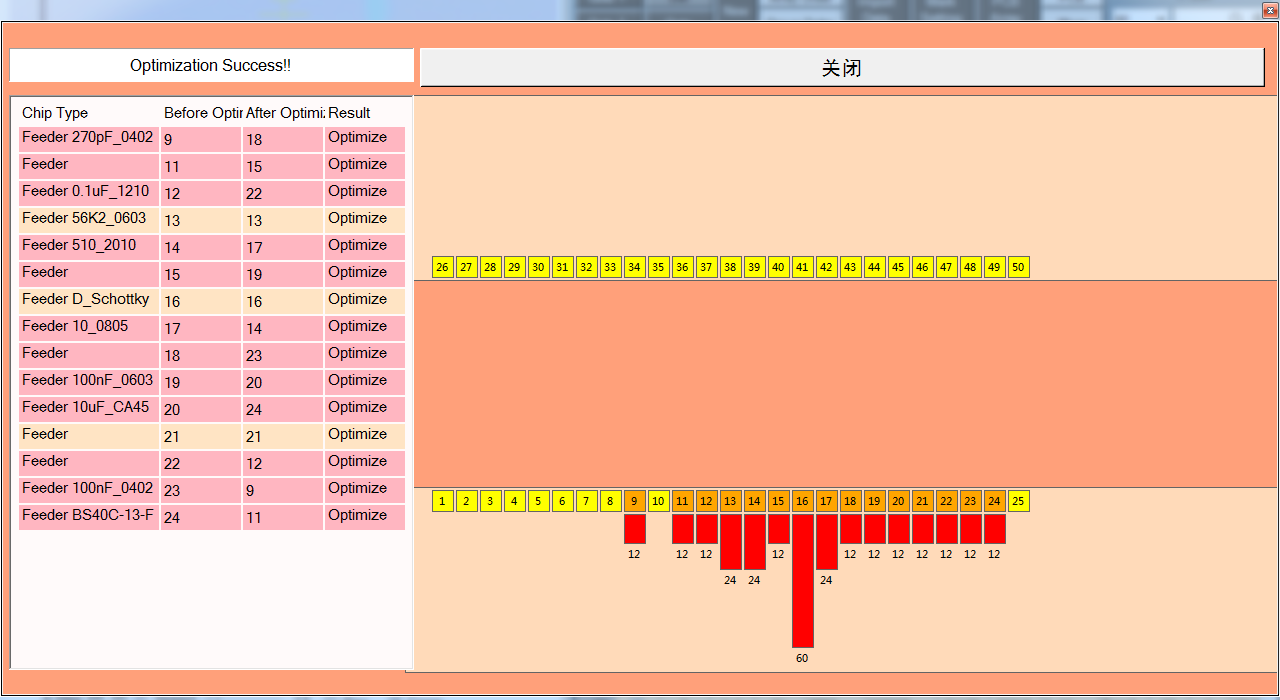
\includegraphics[width=0.8\textwidth]{images/scrot19.png}
 \caption{Generated feeder/slot association}
\end{figure}
Closing this window, the table will be updated with the new feeder/slot values.
\begin{figure}[!htb]
 \centering
 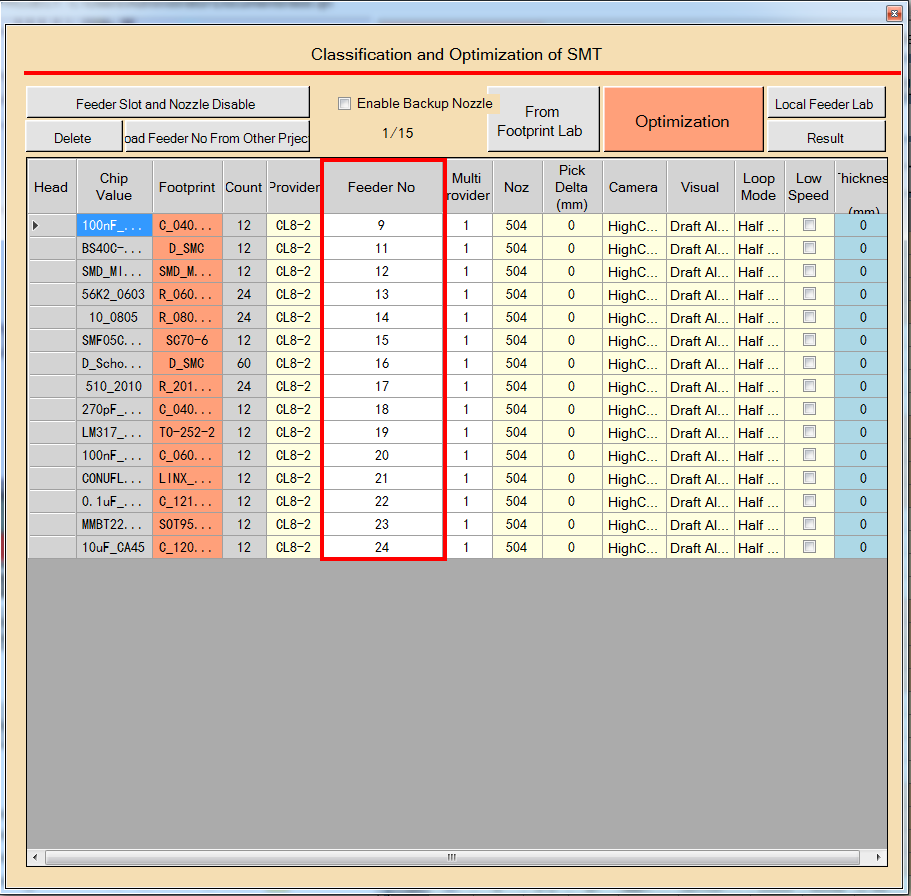
\includegraphics[width=0.85\textwidth]{images/scrot20.png}
 \caption{Feeder optimization table}
\end{figure}
The user must then manually insert every feeder into the appropriate slot.
\newpage
\subsection{Feeder calibration}
After clicking on the \textbf{"Feeder Para"} button the user will be presented with the following configuration window.

\begin{figure}[!htb]
 \centering
 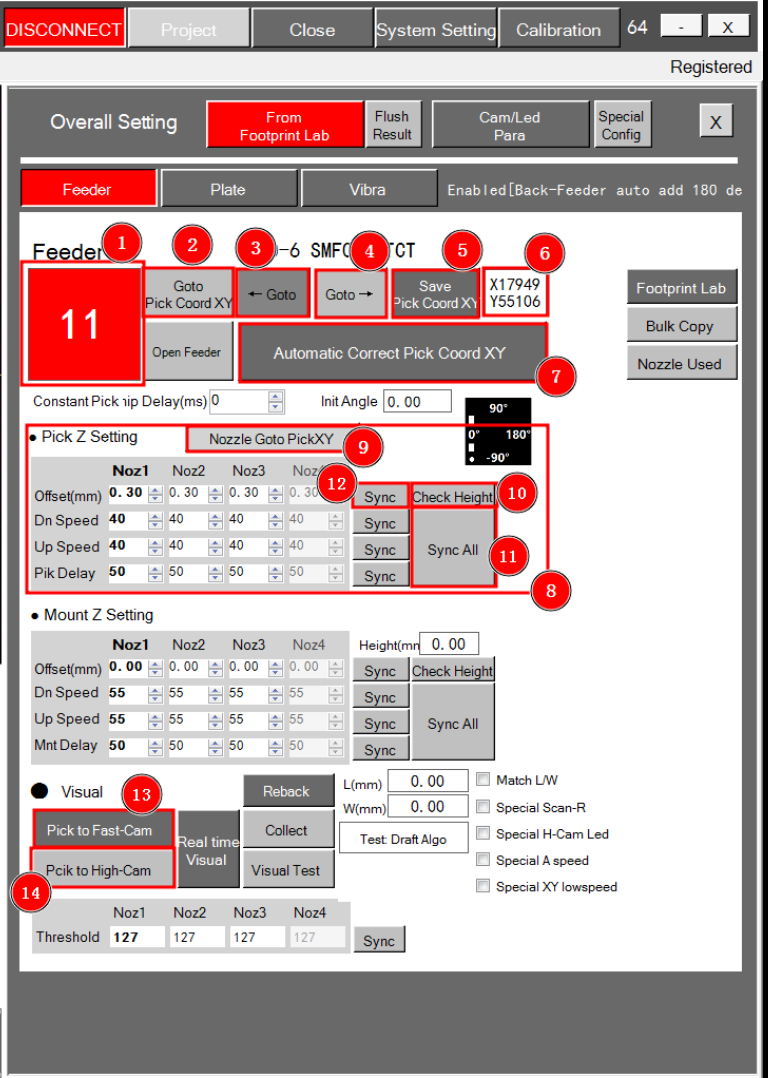
\includegraphics[width=0.95\textwidth]{images/scrot21.png}
 \caption{Feeder calibration tab}
\end{figure}
\newpage
Here's a quick rundown on some important items labeled 1 to 14 on the image:\\

\begin{itemize}
 \item \textbf{1: } Current feeder
 \item \textbf{2: } Move \textbf{Mark Cam} to feeder coordinates.
 \item \textbf{3: } Go to previous feeder.
 \item \textbf{4: } Go to next feeder.
 \item \textbf{5: } Set current \textbf{Mark Cam} coordinates as feeder coordinates.
 \item \textbf{6: } Feeder coordinates.
 \item \textbf{7: } Automatic feeder coordinate calibration helper.
 \item \textbf{8: } Placement head pick up height settings.
 \item \textbf{9: } Move current nozzle to feeder coordinates.
 \item \textbf{10: } Descend nozzle to configured pick up height
 \item \textbf{11: } Sync all fields across nozzles.
 \item \textbf{12: } Sync field across nozzles.
 \item \textbf{13: } Pick up component to \textbf{Fast Cam} for visual inspection.
 \item \textbf{14: } Pick up component to \textbf{High Cam} for visual inspection.
\end{itemize}
The feeder calibration process is relatively straight forward. If the machine's calibration hasn't been tampered with, only minor adjustments are necessary.
\newpage
\subsubsection{Step 1: Verifying the feeder's XY coordinates}
 To verify the feeder's XY coordinates, the user must click on the \textbf{"Goto Pick Coord XY"} button to go. This should move the \textbf{Mark Cam} to where the component is on the feeder.
 If your feeders' pick coordinates are well calibrated, your \textbf{Mark Cam} view should look like this:\\

 \begin{figure}[!htb]
 \centering
 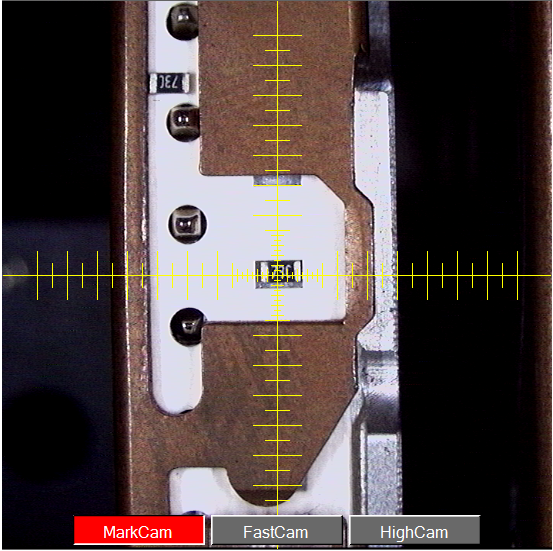
\includegraphics[width=0.6\textwidth]{images/scrot22.png}
 \caption{A well calibrated feeder XY pick coordinates}
\end{figure}
If your XY coordinates are slightly off, you can use the automatic feeder coordinates calibration helper. All you need to do is specify the tape's color.\\

 \begin{figure}[!htb]
 \centering
 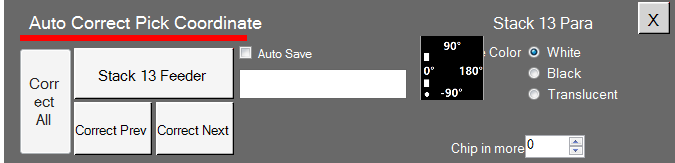
\includegraphics[width=1\textwidth]{images/scrot23.png}
 \caption{The automatic feeder coordinates calibration helper}
\end{figure}
Just press the \textbf{"Stack X Feeder"} (X being the stack's slot number in this case 13). Hit \textbf{"save"} when the \textbf{Mark Cam}'s crosshair is centered on the component and your feeder should be calibrated.
\newpage
\subsubsection{Step 2: Visual inspection}
In the "Visual" section of the feeder calibration tab. The user can setup and run visual inspections using either the \textbf{High Cam} or the \textbf{Fast Cam}.
 \begin{figure}[!htb]
 \centering
 \includegraphics[width=1\textwidth]{images/scrot25.png}
 \caption{The "Visual" section}
\end{figure}
\begin{itemize}
 \item \textbf{1:} Start \textbf{Fast Cam} component inspection.
 \item \textbf{2:} Start \textbf{High Cam} component inspection.
 \item \textbf{3:} Run inspection.
 \item \textbf{4:} Pick up component from feeder.
 \item \textbf{5:} Put component back into feeder.
 \item \textbf{6:} Assert matching between component and footprint dimensions.
\end{itemize}
 \begin{figure}[!htb]
 \centering
 \includegraphics[width=0.6\textwidth]{images/scrot26.png}
 \caption{Visual inspection example}
\end{figure}
\newpage
If your visual inspection fails, try changing the scan radius, threshold and camera light levels in camera settings.\\

 \begin{figure}[!htb]
 \centering
 \includegraphics[width=1\textwidth]{images/scrot27.png}
 \caption{Camera configuration button}
\end{figure}
By clicking on the snapshot you can view the visual inspections' result.
This is especially helpful when trying to diagnose a failed visual inspection.
 \begin{figure}[!htb]
 \centering
 \includegraphics[width=1\textwidth]{images/scrot28.png}
 \caption{Visual inspection snapshot}
\end{figure}
\newpage
 \begin{figure}[!htb]
 \centering
 \includegraphics[width=1\textwidth]{images/scrot29.png}
 \caption{Successful visual inspection result}
\end{figure}
You can click on \textbf{"Size 0"}, \textbf{"Size 1"} and \textbf{"Size 2"} to switch between zoom levels. After the visual inspection succeeds the feeder is good to go.
\newpage
\subsection{Calibrating PCB height}
Lower the nozzles until they touch the PCB then hit \textbf{"Save"} to calibrate PCB height
 \begin{figure}[!htb]
 \centering
 \includegraphics[width=1\textwidth]{images/scrot41.png}
 \caption{PCB Height Calibration}
\end{figure}
\newpage
\subsection{Running jobs}
To navigate to jobs tab click on \textbf{"SMT Run"}.\\

 \begin{figure}[!htb]
 \centering
 \includegraphics[width=1\textwidth]{images/scrot30.png}
 \caption{The \textbf{"SMT Run"} button}
\end{figure}
This should take you to the job tab, on which you can configure different parameters relating to your pick and place jobs, and launch/stop a job.
 \begin{figure}[!htb]
 \centering
 \includegraphics[width=0.6\textwidth]{images/scrot31.png}
 \caption{The job tab}
\end{figure}
\newpage
\begin{itemize}
 \item \textbf{1: } Configure job.
 \item \textbf{2: } Start job.
 \item \textbf{3: } Change pick and place arm speed \& nozzle rotation speed.
 \item \textbf{4: } \textbf{Fast Cam} \& \textbf{High Cam} LEDs only turn on when a visual inspection is ongoing.
 \item \textbf{5: } PCB preview.
\end{itemize}
To configure the job before starting it click on \textbf{"Smt Setting"}, the following window will pop up:
 \begin{figure}[!htb]
 \centering
 \includegraphics[width=0.8\textwidth]{images/scrot32.png}
 \caption{The job configuration window}
\end{figure}
\begin{itemize}
 \item \textbf{1: } Select which feeder is mounted.
 \item \textbf{2: } Select plate feeder start index.
 \item \textbf{3: } Set the number of retries after a failed visual inspection.
 \item \textbf{4: } Set panel mark settings.
\end{itemize}
\newpage
Sometimes not every feeder is mounted, which is accounted for in the Feeder selection window that is accessible by clicking the \textbf{"Is Mount"} button.\\
 \begin{figure}[!htb]
 \centering
 \includegraphics[width=0.8\textwidth]{images/scrot33.png}
 \caption{The feeder selection window}
\end{figure}
Check the box next to each feeder to mark it as mounted.\\

As for plate feeders. If the plate has been used in a previous pick and place job, the first component wont be on row 1 column 1 of the plate, hence the need for a configurable start index. This configuration window can be accessed by clicking the \textbf{"Plate Start Index"} button.
 \begin{figure}[!htb]
 \centering
 \includegraphics[width=0.8\textwidth]{images/scrot34.png}
 \caption{The plate start index configuration window}
\end{figure}
\newpage
\section{Troubleshooting}
In this section we will go over commonly encountered problems and how to approach them.
\begin{table}[!htb]
{\rowcolors{1}{cream1}{cream2}
\begin{tabularx}{\textwidth}{>{\bfseries}l|X}
 \hline
 \makecell{Nozzles not picking up components (especially  \\ nozzle 3 and nozzle 4)} & Check the supplied pressure, the HW-T4-50F requires 100psa (or roughly 6 bars) for proper function \\
 \hline
 Feeder not advancing automatically & Most likely a compressor pressure issue, make sure the machine is being fed the aforementioned 100psa of pressure \\
 \hline
 \makecell{One or more nozzles go to the incorrect feeder\\ Pick XY coordinates despite the mark cam being\\ calibrated properly } & Nozzle Delta calibration issue, check the next section for details \\
 \hline
 \hline
 \makecell{There is an offset when picking to High/Fast Cam }& Fast/High Cam calibration issue, check next section for details \\
 \hline
 \hline
 Chip detection fails & Adjust the Camera Led intensity, range and threshold in the cam settings until it succeeds\\
 \hline
  \makecell{Chip detection succeeds in feeder config but fails\\ at SMT Run }& Uncheck Match L/W in the feeder config window\\
 \hline
 High Cam doesn't show anything & Run visual test, click on fast or mark cam then switch back to high cam\\
 \hline
\end{tabularx}}
\end{table}
\newpage
\section{Calibration and drift correction}
\subsection{Nozzle Delta calibration}
The following procedure is used to correct drift between one or more nozzles and \textbf{Mark Cam}.
\subsubsection{Step 1: install 503 or 504 nozzles on all placement heads}
\subsubsection{Step 2: Place a blank A4 paper}
Place a blank A4 paper on the PCB track, support it with either an empty PCB or a tray so it wont cave in during calibration.
 \begin{figure}[!htb]
 \centering
 \includegraphics[width=0.7\textwidth]{images/a4.jpg}
 \caption{The A4 paper placed on the PCB track}
\end{figure}

\subsubsection{Step 3: Place the ink pot}
Place the inkpot at a place reachable by both the pick and place arm and nozzles.
 \begin{figure}[!htb]
 \centering
 \includegraphics[width=0.7\textwidth]{images/inkpot.jpg}
 \caption{The inkpot placed on top of the High Cam}
\end{figure}
\newpage
\subsubsection{Step 4: Calibrate the write point and dip-ink coordinates}
Place nozzle 1 at the center of the ink pot to get the \textbf{Dip-Ink Coord}. Then lower the nozzle until it touches the ink to get the \textbf{Dip-Ink Height}.\\
Then move nozzle 1 to the top left of the a4 (by a 10mm margin) to get the \textbf{Write-Point XY} and lower the nozzle until it touches the paper to get the \textbf{Write-Point H}.\\
You can sync the height across all nozzles by clicking the the \textbf{"Gen All Write-Point Height"} for \textbf{Write-Point H} and the \textbf{"Gen All Dip-Ink Height"} button for \textbf{Dip-Ink Height}.
 \begin{figure}[!htb]
 \centering
 \includegraphics[width=0.8\textwidth]{images/scrot35.png}
 \caption{The Nozzle Delta calibration window}
\end{figure}
\newpage
\subsubsection{Step 5: Click "Start Write Point" }
This will start the calibration process, where each row of circles will be redrawn four times, the squares in the \textbf{Confirm Center} box will start fading to red. Wait until all rows are finished before proceeding
 \begin{figure}[!htb]
 \centering
 \includegraphics[width=1\textwidth]{images/scrot36.png}
 \caption{The Confirm Center box}
\end{figure}
 \begin{figure}[!htb]
 \centering
 \includegraphics[width=1\textwidth]{images/circles.png}
 \caption{The circles drawn on the paper}
\end{figure}
\newpage
\subsubsection{Step 6: Center Confirm}
Once the machine had stopped. The user must point the \textbf{Mark Cam} at the center of each circle.\\
Click on the uncalibrated (red) square to move the mark cam to where it thinks the corresponding circle is, then correct the offset by pointing the camera at the center of the circle. After doing so click on \textbf{"Center Confirm"}, the square will turn \textbf{green}, then move on to the next uncalibrated (red) square.\\

 \begin{figure}[!htb]
 \centering
 \includegraphics[width=1\textwidth]{images/scrot37.png}
 \caption{Nozzle Delta calibration}
\end{figure}
After calibrating all the points hit \textbf{"Complete"} to finish the Nozzle Delta calibration process.
\newpage
\subsection{High Cam/Fast Cam calibration}
To correct the offset between nozzles and cam centers first start by installing \textbf{solid nozzles} on each of the placement heads. Solid nozzles are a special type of nozzle (with no spring or vacuum hole) used for calibration.\\

 \begin{figure}[!htb]
 \centering
 \includegraphics[width=0.8\textwidth]{images/scrot39.png}
 \caption{A solid nozzle}
\end{figure}
\newpage
For the \textbf{High Cam}, calibration may be done on a per nozzle basis. Or in an automated manner.\\
For per nozzle calibration, place the desired nozzle near the \textbf{High Cam}s' cent and click \textbf{"Noz X Calibration"} with X being the selected nozzle number.\\
For auto calibration place nozzle 1 near the \textbf{High Cam}s' center and click \textbf{"Auto Calibration"}. This will calibrate all four nozzles without manual intervention.\\

\begin{figure}[!htb]
 \centering
 \includegraphics[width=0.8\textwidth]{images/scrot38.png}
 \caption{High Camera calibration}
\end{figure}
To calibrate the \textbf{Fast Cam} place nozzle 1 at the center of its' corresponding \textbf{Fast Cam} crosshair and click \textbf{"Auto Calibration"}.\\

 \begin{figure}[!htb]
 \centering
 \includegraphics[width=0.8\textwidth]{images/scrot40.png}
 \caption{Fast Camera calibration}
\end{figure}
\textbf{Note: } Each nozzles takes around 2 and a half minutes to calibrate.
\end{document}
